%%% -*-LaTeX-*-
%%% ====================================================================
%%% This is a sample top-level LaTeX-2e file for typesetting a thesis
%%% or dissertation at the University of Utah.  Most students find it
%%% convenient to start with a COPY of this file as a template, and
%%% then alter that copy to match their needs.
%%%
%%% There is an associated Unix Makefile that can be similarly
%%% customized, and then the only command ever needed to typeset the
%%% complete thesis is the single word "make".  Of course, during
%%% writing and typesetting, not all of the steps are needed, so
%%% often, one can just name a convenience target such as "make
%%% dvi-pass" or "make pdf-pass" to do just a single pass of LaTeX and
%%% BibTeX.
%%%
%%% There should be no, or very few, macro definitions in this file;
%%% any needed belong in a private style file, called mythesis.sty,
%%% and input below after all other packages.  The bulk of this file
%%% should just be command invocations, and any arguments that they
%%% need.
%%%
%%% We exploit the fact that TeX ignores spaces after command names to
%%% line up arguments for better readability.
%%%
%%% Each chapter should be a separate complete file, so that you can
%%% insert a command like \includeonly{chap_intro} before the first
%%% \include{chap_xxx} command to avoid typesetting all but the
%%% chapter that you are currently working on, to save time.
%%%
%%% Remember that occupants of job positions change jobs from time to
%%% time: YOU are responsible for ensuring correct names of all humans
%%% mentioned in this file!
%%%
%%% [16-Mar-2016]
%%% ====================================================================

\documentclass[11pt,Chicago]{uuthesis2e}

%%% Undefine two macros from uuthesis2e.cls that conflict with
%%% definitions in amsthm.sty that fail to check for prior definitions!
%%% NB: The amsthm package refines the LaTeX theorem environment,
%%% and the uuthesis-color-headings wraps that definition, so the
%%% amsthm package must be read first!
\let \proof    = \relax
\let \endproof = \relax
\usepackage {amsthm}

%%% ====================================================================
%%% Choose an alternate font family for the document if the TeX default
%%% of Computer Modern is not wanted:

\usepackage{mathpazo}

%%% ====================================================================
%%% Some miscellaneous Utah- and student-specific settings:
%%%
%%% Chapter is one level, section and subsection are the next two levels.

\fourlevels

%%% ====================================================================
%%% The remaining packages are required by this particular thesis,
%%% but other theses will almost certainly need different packages:
%%%
%%% WARNING: MANY \LaTeX{} packages change dimensions, glue, and/or
%%% formatting styles, and such changes are likely to conflict with
%%% University of Utah Thesis Office requirements.  Therefore, minimize
%%% the number of packages that you include!

\usepackage {amsmath}
\usepackage {amssymb}
\usepackage {bm}
\usepackage {bibnames}
\usepackage {citesort}
\usepackage {graphicx}
\usepackage {graphpap}
\usepackage {longtable}
\usepackage {multirow}
\usepackage {tikz}
\usetikzlibrary {decorations.markings}
\usepackage {varioref}

%%% ====================================================================
%%% Support for a subject index:

%% \usepackage {uuthesis-index}

%%% ====================================================================
%%% The various uuthesis-*.sty packages must come AFTER all other
%%% system-provided packages, so that they can correctly override
%%% settings from those packages.

%%% Include latest updates for 2016 (WARNING: the name is subject to
%%% change: see http://www.math.utah.edu/pub/uuthesis/ for the most
%%% current version.)

\usepackage {uuthesis-2016-h}  % MANDATORY package

%%% This is an OPTIONAL package that sets chapter and sectional headings
%%% in color:
%%% Use one or the other of these:
% \usepackage {color}
%%: \usepackage {uuthesis-color-headings}
%%: \definecolor{utahheadingcolor} {rgb}  {0.7, 0.0, 0.0}
%%: \definecolor{utahtheoremcolor} {rgb}  {0.490,0.149,0.804} % purple4
%%: \definecolor{utahtheoremcolor} {rgb}  {0.545,0.137,0.137} % brown4

%%% Here is another, and more convenient, way to define colors, via
%%% aliases of named colors in the X11-derived rgb.sty file

%%: \usepackage{coloralias}
%%: \definecoloralias{utahheadingcolor}{steelblue4}
%%: \definecoloralias{utahtheoremcolor}{hotpink3}

%%% The default heading color is utahred (defined by University Printing
%%% Services as 0.8 red, 0.0 green, 0.0 blue), but you could redefine
%%% that to, for example, a dark blue color, like this AFTER including
%%% the package:
%%%
%%%     \definecolor{utahheading}{rgb}{0,0,0.8}
%%%
%%% NB: Be careful with use of colors in typesetting, and in figures,
%%% because about 6 percent of the human male population is red/green
%%% color blind: they see those colors as shades of brown.  Red and
%%% blue, or blue and green, are better choices for choosing
%%% distinguishable colors.  Also, avoid light colors, especially
%%% yellow, because they are hard to see against white paper and
%%% screen backgrounds, and when printed on black-and-white printers,
%%% where they are rendered in gray, they may be too faint to read.

%%% ====================================================================
%%% Support for a subject index:
%
%: \usepackage {uuthesis-index}

%%% ====================================================================
%%% This single user-specific file is where all personal customizations
%%% and macro definitions should be placed, and it should come LAST,
%%% after ALL OTHER packages, in case it needs to override some of their
%%% definitions.

\usepackage{listings}
\usepackage{subfig}
\usepackage {mythesis}


%%% ====================================================================
%%% The student-specific front matter fields are defined here:

\author                 {Anastasia Cherkaev}
\title                  {SWEETPEA: A LANGUAGE FOR EXPERIMENTAL DESIGN}
\thesistype             {thesis}

\dedication             {For my parents; I'm sorry this thesis doesn't contain a single theorem.}

%%% Most students need just a short degree name, like this:
\degree                 {Master of Science \\
                         in  \\
                         Computer Science}
%%% However, multiline degrees are possible, and are done like this:
%%% \degree                 {Doctor of Philosophy \\
%%%                         in \\
%%%                         Mathematical Physics}

%%% College- and Department-level definitions:
\approvaldepartment     {Computer Science}
\department             {Department of Computer Science}
\graduatedean           {David Kieda}
\departmentchair        {Ross Whitaker}

%%% The graduate student's committee members:
\committeechair         {Vivek Srikumar}
\firstreader            {Matthew Flatt}
\secondreader           {Jonathan Cohen}
\thirdreader            {none}
\fourthreader           {none}
\chairtitle             {Professor}

%%% NB: It is rare, but possible, for there to be two chairs, For
%%% example, one student had
%%%
%%% \committeechair{\mbox{\small Andrej Cherkaev and Andrejs Treibergs}}
%%%
%%% The \mbox{} ensures that line breaks cannot happen, and the \small
%%% is necessary to make the names fit on the Dissertation Approval form

%%% Dates that must be adjusted for each academic term, and be permitted
%%% according to the University of Utah Thesis Office:
\submitdate             {November 2018}
\copyrightyear          {2018}

%%% Dates on which committee members approved the thesis
\chairdateapproved      {26 Nov 2018}
\firstdateapproved      {26 Nov 2018}
\seconddateapproved     {26 Nov 2018}
\thirddateapproved      {26 Nov 2018}
\fourthdateapproved     {26 Nov 2018}

%%% ====================================================================
%%% Typesetting begins here:

\begin{document}

%% Comment out items by inserting a percent % character
\frontmatterformat
\titlepage
\copyrightpage
\dissertationapproval
\setcounter {page}     {2}             % UofU Thesis Office demands abstract on p. iii: start one lower
\preface    {abstract} {Abstract}
\dedicationpage
\tableofcontents
\listoffigures
\listoftables
%
%%% Optional front matter page(s), made from source "notation.tex". If
%%% you don't need it, then comment out the \optionalfront command
%%% line!  The first argument is the (unnumbered) section header for
%%% the text supplied by the file input by the second argument; that
%%% file must NOT contain \chapter, \section, \subsection, \ldots{}
%%% sectioning commands.

\optionalfront {Notation and Symbols} {%%% -*-LaTeX-*-
%%%
%%% This is notation.tex.
%%%
%%% This file is included in a thesis with a front-matter command
%%%
%%%     \optionalfront {Notation and Symbols} {%%% -*-LaTeX-*-
%%%
%%% This is notation.tex.
%%%
%%% This file is included in a thesis with a front-matter command
%%%
%%%     \optionalfront {Notation and Symbols} {%%% -*-LaTeX-*-
%%%
%%% This is notation.tex.
%%%
%%% This file is included in a thesis with a front-matter command
%%%
%%%     \optionalfront {Notation and Symbols} {\input{notation}}
%%%
%%% The heading for this material is provided by the first argument
%%% so none needs to be supplied here.

\begin{tabular}{ll}
    \hline
    $\alpha$      & fine-structure (dimensionless) constant, approximately $1 / 137$ \\
    $\alpha$      & radiation of doubly-ionized helium ions, He++ \\
    $\beta$       & radiation of electrons \\
    $\gamma$      & radiation of very high frequency, beyond that of X rays \\
    $\gamma$      & Euler's constant, approximately $0.577\,215\,\ldots{}$  \\
    $\delta$      & stepsize in numerical integration \\
    $\delta(x)$   & Dirac's famous function \\
    $\epsilon$    & a tiny number, usually in the context of a limit to zero \\
    $\zeta(x)$    & the famous Riemann zeta function \\
    \ldots{}      & \ldots{}  \\
    $\psi(x)$     & logarithmic derivative of the gamma function \\
    $\omega$      & frequency \\
    \hline
\end{tabular}
}
%%%
%%% The heading for this material is provided by the first argument
%%% so none needs to be supplied here.

\begin{tabular}{ll}
    \hline
    $\alpha$      & fine-structure (dimensionless) constant, approximately $1 / 137$ \\
    $\alpha$      & radiation of doubly-ionized helium ions, He++ \\
    $\beta$       & radiation of electrons \\
    $\gamma$      & radiation of very high frequency, beyond that of X rays \\
    $\gamma$      & Euler's constant, approximately $0.577\,215\,\ldots{}$  \\
    $\delta$      & stepsize in numerical integration \\
    $\delta(x)$   & Dirac's famous function \\
    $\epsilon$    & a tiny number, usually in the context of a limit to zero \\
    $\zeta(x)$    & the famous Riemann zeta function \\
    \ldots{}      & \ldots{}  \\
    $\psi(x)$     & logarithmic derivative of the gamma function \\
    $\omega$      & frequency \\
    \hline
\end{tabular}
}
%%%
%%% The heading for this material is provided by the first argument
%%% so none needs to be supplied here.

\begin{tabular}{ll}
    \hline
    $\alpha$      & fine-structure (dimensionless) constant, approximately $1 / 137$ \\
    $\alpha$      & radiation of doubly-ionized helium ions, He++ \\
    $\beta$       & radiation of electrons \\
    $\gamma$      & radiation of very high frequency, beyond that of X rays \\
    $\gamma$      & Euler's constant, approximately $0.577\,215\,\ldots{}$  \\
    $\delta$      & stepsize in numerical integration \\
    $\delta(x)$   & Dirac's famous function \\
    $\epsilon$    & a tiny number, usually in the context of a limit to zero \\
    $\zeta(x)$    & the famous Riemann zeta function \\
    \ldots{}      & \ldots{}  \\
    $\psi(x)$     & logarithmic derivative of the gamma function \\
    $\omega$      & frequency \\
    \hline
\end{tabular}
}

%%% Uncomment this is you want the contents of acknowledge.tex typeset here.
%%% Note that both "Acknowledgement" and "Acknowledgment" are accepted
%%% spellings of that word.

% \preface{acknowledge}{Acknowledgements}

%%% Demonstrations of thesis typesetting features for the sample thesis.
%%% Once you have seen the examples, you can comment out this line.
%%: \optionalfront {Typesetting Experiments} {%%% -*-LaTeX-*-
%%% ====================================================================
%%% This file is intended to be included as a front-matter section of
%%% the sample thesis, with a command like this
%%%
%%% \optionalfront{Typesetting Experiments}{%%% -*-LaTeX-*-
%%% ====================================================================
%%% This file is intended to be included as a front-matter section of
%%% the sample thesis, with a command like this
%%%
%%% \optionalfront{Typesetting Experiments}{%%% -*-LaTeX-*-
%%% ====================================================================
%%% This file is intended to be included as a front-matter section of
%%% the sample thesis, with a command like this
%%%
%%% \optionalfront{Typesetting Experiments}{\input{samples}}
%%%
%%% just before the \maintext macro that begins the body of the thesis,
%%% and starts chapter numbering.
%%%
%%% [16-Mar-2016]
%%% ====================================================================

\input{rgb.sty}

\definecolor{utahred} {rgb} {0.8, 0.0, 0.0} % official definition for University of Utah Printing Services

\doublespace

%% \showthe \baselineskip

In this section, we use color in several places.
The \verb=\colorbox= command takes two arguments
--- a named color and text to be in black on a
background of that color --- and sets the text in
a box with a small margin of width \verb=\fboxsep=
(set to \texttt{\the\fboxsep} in this document).

Here, we want a tighter colored box that has a
fixed height, and is independent of letter shape.
We set the margin to zero inside a group so that
the change is purely local, and so that height and
depth of the line are not increased over what they
would be if the colored box were not used.  We
prefix a \TeX{} \verb=\strut= to the user-supplied
text, because that command expands to a zero-width
box of the height and depth of parentheses, which,
in most fonts, delimit the extent of letter
shapes.

\begin{verbatim}
\newcommand {\hilitebox} [1] {{\fboxsep = 0pt\colorbox{pink}{\strut #1}}}
\end{verbatim}

\newcommand {\hilitebox} [1] {{\fboxsep = 0pt\colorbox{pink}{\strut #1}}}

Here is a fragment from the first chapter in another
thesis, set in \emph{emphasized text} to distinguish it
from the rest of this section:

\begin{itshape}
    In light of the known results, the consistency
    of empirical semivariogram and related
    estimators is widely considered a settled
    matter.  For example, Lahiri, Lee, and Cressie
    \cite{Lahiri:2002:ADA} state:

    \begin{quote}
        The simpler and more commonly used
        nonparametric estimators of the variogram,
        such as the method of moments estimator of
        Matheron (1962) and its robustified
        versions due to Cressie and Hawkins (1980)
        have many desirable properties like,
        unbiasedness, consistency, etc. \ldots
    \end{quote}
    \noindent
    Regarding a kernel estimator of the covariance
    function, Hall and Patil
    \cite{Hall:1994:PNE} remarked:
    \begin{quote}
        It is not difficult to see that if, as $ n
        $ increases, the points $ t_i $ become
        increasingly dense in each bounded subset
        of $ \mathbb{R}^d $, then the bandwidth $
        h $ may be chosen so that $ \check \rho(t)
        \to \rho(t) $ as $ n \to \infty $, for
        each $ t \in \mathbb{R}^d $.
    \end{quote}
    However, in order to be true, such statements
    would need to be qualified by many assumptions
    on the random field as well as on the
    observation locations. We will see in
    \S2.3 that even for well-behaved
    random fields (e.g., $\rho^*$-mixing Gaussian
    random fields), it is not enough to assume
    that the observation locations become
    increasingly dense in each bounded subset; a
    stronger assumption must be made to ensure
    that the observation locations do not become
    denser in one region too much faster than in
    others.
\end{itshape}

The text before the previous paragraph contained
two \texttt{quote} environments separated by a
line of prose.  Here are some more tests of both
kinds of \LaTeX{} environments for showing text
written by someone else.

This is a \hilitebox{\texttt{quote}} environment
with one short line, following a fairly short
paragraph of prose (in this, and following
examples, the text is explicitly colored with a
command like \verb=\color{purple}= inside the
environment before the text):
%
\begin{singlespace}
\color{darkblue}
\begin{verbatim}
\begin{quote}
    \color{purple}
    14 March 2016 is $\pi \approx 3.1416$ day in funny notation.
    \hfill \emph{Web news reports}
\end{quote}
\end{verbatim}
\end{singlespace}
%
\begin{quote}
    \color{purple}
    14 March 2016 is $\pi \approx 3.1416$ day in funny notation.
    \hfill \emph{Web news reports}
\end{quote}

This is a \hilitebox{\texttt{quote}} environment
with three short lines, each a separate paragraph,
following a fairly short paragraph of prose.

\begin{singlespace}
\color{darkblue}
\begin{verbatim}
\begin{quote}
    \color{forestgreen}
    14 March 2016 is $\pi \approx 3.1416$ day in funny notation.
    \hfill \emph{Web news reports}

    14 March 2016 is $\pi \approx 3.1416$ day in funny notation.
    \hfill \emph{Web news reports}

    14 March 2016 is $\pi \approx 3.1416$ day in funny notation.
    \hfill \emph{Web news reports}
\end{quote}
\end{verbatim}
\end{singlespace}
%
\begin{quote}
    \color{forestgreen}
    14 March 2016 is $\pi \approx 3.1416$ day in funny notation.
    \hfill \emph{Web news reports}

    14 March 2016 is $\pi \approx 3.1416$ day in funny notation.
    \hfill \emph{Web news reports}

    14 March 2016 is $\pi \approx 3.1416$ day in funny notation.
    \hfill \emph{Web news reports}
\end{quote}

Here is another example, this time with separate
colors for each paragraph:

\begin{singlespace}
\color{darkblue}
\begin{verbatim}
\begin{quote}
    \color{darkkhaki}
    14 March 2016 is $\pi \approx 3.1416$ day in funny notation.
    \hfill \emph{Web news reports}

    \color{darkmagenta}
    14 March 2016 is $\pi \approx 3.1416$ day in funny notation.
    \hfill \emph{Web news reports}

    \color{darkcyan}
    14 March 2016 is $\pi \approx 3.1416$ day in funny notation.
    \hfill \emph{Web news reports}

    \color{darkorange}
    14 March 2016 is $\pi \approx 3.1416$ day in funny notation.
    14 March 2016 is $\pi \approx 3.1416$ day in funny notation.
    14 March 2016 is $\pi \approx 3.1416$ day in funny notation.
    \linebreak
    \strut
    \hfill \emph{Web news reports}
\end{quote}
\end{verbatim}
\end{singlespace}
%
\begin{quote}
    \color{darkkhaki}
    14 March 2016 is $\pi \approx 3.1416$ day in funny notation.
    \hfill \emph{Web news reports}

    \color{darkmagenta}
    14 March 2016 is $\pi \approx 3.1416$ day in funny notation.
    \hfill \emph{Web news reports}

    \color{darkcyan}
    14 March 2016 is $\pi \approx 3.1416$ day in funny notation.
    \hfill \emph{Web news reports}

    \color{darkorange}
    14 March 2016 is $\pi \approx 3.1416$ day in funny notation.
    14 March 2016 is $\pi \approx 3.1416$ day in funny notation.
    14 March 2016 is $\pi \approx 3.1416$ day in funny notation.
    \linebreak
    \strut
    \hfill \emph{Web news reports}
\end{quote}

Notice that \hilitebox{\texttt{quote}} paragraphs
are \emph{not} indented, but the environment
itself \emph{is} indented on the left and right by
the value of \verb=\leftmargin= (set to
\texttt{\the\leftmargin} in this document, which
should be identical to \verb=2.5em=, where
\verb=1em= = \texttt{\dimen0 = 1em \the\dimen0}).

For debugging purposes, we also have
\verb=\leftmargini= set to
\texttt{\the\leftmargini}, and we have
\verb=\leftmarginii= set to
\texttt{\the\leftmarginii}.

This is a \hilitebox{\texttt{quotation}}
environment with one paragraph, following a fairly
short paragraph of prose (notice that the
\texttt{quotation} paragraphs \emph{are}
indented):

\begin{singlespace}
\color{darkblue}
\begin{verbatim}
\begin{quotation}
    \color{blue}
    Algebra is concerned with manipulation in
    \emph{time}, and geometry is concerned with
    \emph{space}. These are two orthogonal aspects
    of the world, and they represent two different
    points of view in mathematics.  Thus the
    argument or dialogue between mathematicians in
    the past about the relative importance of
    geometry and algebra represents something very
    fundamental.
    \hfill
    \emph{Sir Michael Atiyah}
    % Mathematics in the 20$^{th}$ century
    % NTM {\bf 10}(1--3) 25--39 (September 2002)
    % http://dx.doi.org/10.1007/BF03033096
\end{quotation}
\end{verbatim}
\end{singlespace}
%
\begin{quotation}
    \color{blue}
    Algebra is concerned with manipulation in
    \emph{time}, and geometry is concerned with
    \emph{space}. These are two orthogonal aspects
    of the world, and they represent two different
    points of view in mathematics.  Thus the
    argument or dialogue between mathematicians in
    the past about the relative importance of
    geometry and algebra represents something very
    fundamental.
    \hfill
    \emph{Sir Michael Atiyah}
    % Mathematics in the 20$^{th}$ century
    % NTM {\bf 10}(1--3) 25--39 (September 2002)
    % http://dx.doi.org/10.1007/BF03033096
\end{quotation}

This is a \hilitebox{\texttt{quotation}} environment with three
paragraphs, following a fairly short paragraph of prose:

\begin{quotation}
    \color{utahred}
    Algebra is concerned with manipulation in
    \emph{time}, and geometry is concerned with
    \emph{space}. These are two orthogonal aspects
    of the world, and they represent two different
    points of view in mathematics.  Thus the
    argument or dialogue between mathematicians in
    the past about the relative importance of
    geometry and algebra represents something very
    fundamental.
    \hfill
    \emph{Sir Michael Atiyah}

    Algebra is concerned with manipulation in
    \emph{time}, and geometry is concerned with
    \emph{space}. These are two orthogonal aspects
    of the world, and they represent two different
    points of view in mathematics.  Thus the
    argument or dialogue between mathematicians in
    the past about the relative importance of
    geometry and algebra represents something very
    fundamental.
    \hfill
    \emph{Sir Michael Atiyah}

    Algebra is concerned with manipulation in
    \emph{time}, and geometry is concerned with
    \emph{space}. These are two orthogonal aspects
    of the world, and they represent two different
    points of view in mathematics.  Thus the
    argument or dialogue between mathematicians in
    the past about the relative importance of
    geometry and algebra represents something very
    fundamental.
    \hfill
    \emph{Sir Michael Atiyah}
\end{quotation}

%% \showthe \baselineskip

Now all following text should be back in
double-spaced mode, and just go on and on and on
and on and on and on and on and on and on and on
and on and on and on and on and on and on and on
and on and on and on and on and on and on and on
and on and on and on and on and on and on and on
and on and on and on and on and on and on and on
and on and on and on and on and on and on and on
and on and on and on and on and on and on and on
and on and on and on and on and on and on and on
and on and on and on and on and on and on and on
and on and on and on and on and on and on and on
and on and on and on and on \ldots{}.

%% \showthe \baselineskip

Now all following text should be back in
double-spaced mode, and just go on and on and on
and on and on and on and on and on and on and on
and on and on and on and on and on and on and on
and on and on and on and on and on and on and on
and on and on and on and on and on and on and on
and on and on and on and on and on and on and on
and on and on and on and on and on and on and on
and on and on and on and on and on and on and on
and on and on and on and on and on and on and on
and on and on and on and on and on and on and on
and on and on and on and on and on and on and on
and on and on and on and on \ldots{}.

%%% \showthe \baselineskip
}
%%%
%%% just before the \maintext macro that begins the body of the thesis,
%%% and starts chapter numbering.
%%%
%%% [16-Mar-2016]
%%% ====================================================================

%% Derived from file://ibapah.math.utah.edu/usr/lib/X11/rgb.txt
%% on Wed Jun  9 11:48:18 MDT 2004
%% by ~beebe/src/awk/rgb.awk

\definecolor{aliceblue}{rgb}{0.941,0.973,1}                    	% #f0f8ff 240 248 255 AliceBlue
\definecolor{antiquewhite1}{rgb}{1,0.937,0.859}                	% #ffefdb 255 239 219 AntiqueWhite1
\definecolor{antiquewhite2}{rgb}{0.933,0.875,0.800}            	% #eedfcc 238 223 204 AntiqueWhite2
\definecolor{antiquewhite3}{rgb}{0.804,0.753,0.690}            	% #cdc0b0 205 192 176 AntiqueWhite3
\definecolor{antiquewhite4}{rgb}{0.545,0.514,0.471}            	% #8b8378 139 131 120 AntiqueWhite4
\definecolor{antiquewhite}{rgb}{0.980,0.922,0.843}             	% #faebd7 250 235 215 AntiqueWhite
\definecolor{aquamarine1}{rgb}{0.498,1,0.831}                  	% #7fffd4 127 255 212 aquamarine1
\definecolor{aquamarine2}{rgb}{0.463,0.933,0.776}              	% #76eec6 118 238 198 aquamarine2
\definecolor{aquamarine3}{rgb}{0.400,0.804,0.667}              	% #66cdaa 102 205 170 aquamarine3
\definecolor{aquamarine4}{rgb}{0.271,0.545,0.455}              	% #458b74 69 139 116 aquamarine4
\definecolor{aquamarine}{rgb}{0.498,1,0.831}                   	% #7fffd4 127 255 212 aquamarine
\definecolor{azure1}{rgb}{0.941,1,1}                           	% #f0ffff 240 255 255 azure1
\definecolor{azure2}{rgb}{0.878,0.933,0.933}                   	% #e0eeee 224 238 238 azure2
\definecolor{azure3}{rgb}{0.757,0.804,0.804}                   	% #c1cdcd 193 205 205 azure3
\definecolor{azure4}{rgb}{0.514,0.545,0.545}                   	% #838b8b 131 139 139 azure4
\definecolor{azure}{rgb}{0.941,1,1}                            	% #f0ffff 240 255 255 azure
\definecolor{beige}{rgb}{0.961,0.961,0.863}                    	% #f5f5dc 245 245 220 beige
\definecolor{bisque1}{rgb}{1,0.894,0.769}                      	% #ffe4c4 255 228 196 bisque1
\definecolor{bisque2}{rgb}{0.933,0.835,0.718}                  	% #eed5b7 238 213 183 bisque2
\definecolor{bisque3}{rgb}{0.804,0.718,0.620}                  	% #cdb79e 205 183 158 bisque3
\definecolor{bisque4}{rgb}{0.545,0.490,0.420}                  	% #8b7d6b 139 125 107 bisque4
\definecolor{bisque}{rgb}{1,0.894,0.769}                       	% #ffe4c4 255 228 196 bisque
\definecolor{black}{rgb}{0,0,0}                                	% #000000 0 0 0 black
\definecolor{blanchedalmond}{rgb}{1,0.922,0.804}               	% #ffebcd 255 235 205 BlanchedAlmond
\definecolor{blue1}{rgb}{0,0,1}                                	% #0000ff 0 0 255 blue1
\definecolor{blue2}{rgb}{0,0,0.933}                            	% #0000ee 0 0 238 blue2
\definecolor{blue3}{rgb}{0,0,0.804}                            	% #0000cd 0 0 205 blue3
\definecolor{blue4}{rgb}{0,0,0.545}                            	% #00008b 0 0 139 blue4
\definecolor{blue}{rgb}{0,0,1}                                 	% #0000ff 0 0 255 blue
\definecolor{blueviolet}{rgb}{0.541,0.169,0.886}               	% #8a2be2 138 43 226 BlueViolet
\definecolor{brown1}{rgb}{1,0.251,0.251}                       	% #ff4040 255 64 64 brown1
\definecolor{brown2}{rgb}{0.933,0.231,0.231}                   	% #ee3b3b 238 59 59 brown2
\definecolor{brown3}{rgb}{0.804,0.200,0.200}                   	% #cd3333 205 51 51 brown3
\definecolor{brown4}{rgb}{0.545,0.137,0.137}                   	% #8b2323 139 35 35 brown4
\definecolor{brown}{rgb}{0.647,0.165,0.165}                    	% #a52a2a 165 42 42 brown
\definecolor{burlywood1}{rgb}{1,0.827,0.608}                   	% #ffd39b 255 211 155 burlywood1
\definecolor{burlywood2}{rgb}{0.933,0.773,0.569}               	% #eec591 238 197 145 burlywood2
\definecolor{burlywood3}{rgb}{0.804,0.667,0.490}               	% #cdaa7d 205 170 125 burlywood3
\definecolor{burlywood4}{rgb}{0.545,0.451,0.333}               	% #8b7355 139 115 85 burlywood4
\definecolor{burlywood}{rgb}{0.871,0.722,0.529}                	% #deb887 222 184 135 burlywood
\definecolor{cadetblue1}{rgb}{0.596,0.961,1}                   	% #98f5ff 152 245 255 CadetBlue1
\definecolor{cadetblue2}{rgb}{0.557,0.898,0.933}               	% #8ee5ee 142 229 238 CadetBlue2
\definecolor{cadetblue3}{rgb}{0.478,0.773,0.804}               	% #7ac5cd 122 197 205 CadetBlue3
\definecolor{cadetblue4}{rgb}{0.325,0.525,0.545}               	% #53868b 83 134 139 CadetBlue4
\definecolor{cadetblue}{rgb}{0.373,0.620,0.627}                	% #5f9ea0 95 158 160 CadetBlue
\definecolor{chartreuse1}{rgb}{0.498,1,0}                      	% #7fff00 127 255 0 chartreuse1
\definecolor{chartreuse2}{rgb}{0.463,0.933,0}                  	% #76ee00 118 238 0 chartreuse2
\definecolor{chartreuse3}{rgb}{0.400,0.804,0}                  	% #66cd00 102 205 0 chartreuse3
\definecolor{chartreuse4}{rgb}{0.271,0.545,0}                  	% #458b00 69 139 0 chartreuse4
\definecolor{chartreuse}{rgb}{0.498,1,0}                       	% #7fff00 127 255 0 chartreuse
\definecolor{chocolate1}{rgb}{1,0.498,0.141}                   	% #ff7f24 255 127 36 chocolate1
\definecolor{chocolate2}{rgb}{0.933,0.463,0.129}               	% #ee7621 238 118 33 chocolate2
\definecolor{chocolate3}{rgb}{0.804,0.400,0.114}               	% #cd661d 205 102 29 chocolate3
\definecolor{chocolate4}{rgb}{0.545,0.271,0.075}               	% #8b4513 139 69 19 chocolate4
\definecolor{chocolate}{rgb}{0.824,0.412,0.118}                	% #d2691e 210 105 30 chocolate
\definecolor{coral1}{rgb}{1,0.447,0.337}                       	% #ff7256 255 114 86 coral1
\definecolor{coral2}{rgb}{0.933,0.416,0.314}                   	% #ee6a50 238 106 80 coral2
\definecolor{coral3}{rgb}{0.804,0.357,0.271}                   	% #cd5b45 205 91 69 coral3
\definecolor{coral4}{rgb}{0.545,0.243,0.184}                   	% #8b3e2f 139 62 47 coral4
\definecolor{coral}{rgb}{1,0.498,0.314}                        	% #ff7f50 255 127 80 coral
\definecolor{cornflowerblue}{rgb}{0.392,0.584,0.929}           	% #6495ed 100 149 237 CornflowerBlue
\definecolor{cornsilk1}{rgb}{1,0.973,0.863}                    	% #fff8dc 255 248 220 cornsilk1
\definecolor{cornsilk2}{rgb}{0.933,0.910,0.804}                	% #eee8cd 238 232 205 cornsilk2
\definecolor{cornsilk3}{rgb}{0.804,0.784,0.694}                	% #cdc8b1 205 200 177 cornsilk3
\definecolor{cornsilk4}{rgb}{0.545,0.533,0.471}                	% #8b8878 139 136 120 cornsilk4
\definecolor{cornsilk}{rgb}{1,0.973,0.863}                     	% #fff8dc 255 248 220 cornsilk
\definecolor{cyan1}{rgb}{0,1,1}                                	% #00ffff 0 255 255 cyan1
\definecolor{cyan2}{rgb}{0,0.933,0.933}                        	% #00eeee 0 238 238 cyan2
\definecolor{cyan3}{rgb}{0,0.804,0.804}                        	% #00cdcd 0 205 205 cyan3
\definecolor{cyan4}{rgb}{0,0.545,0.545}                        	% #008b8b 0 139 139 cyan4
\definecolor{cyan}{rgb}{0,1,1}                                 	% #00ffff 0 255 255 cyan
\definecolor{darkblue}{rgb}{0,0,0.545}                         	% #00008b 0 0 139 DarkBlue
\definecolor{darkcyan}{rgb}{0,0.545,0.545}                     	% #008b8b 0 139 139 DarkCyan
\definecolor{darkgoldenrod1}{rgb}{1,0.725,0.059}               	% #ffb90f 255 185 15 DarkGoldenrod1
\definecolor{darkgoldenrod2}{rgb}{0.933,0.678,0.055}           	% #eead0e 238 173 14 DarkGoldenrod2
\definecolor{darkgoldenrod3}{rgb}{0.804,0.584,0.047}           	% #cd950c 205 149 12 DarkGoldenrod3
\definecolor{darkgoldenrod4}{rgb}{0.545,0.396,0.031}           	% #8b6508 139 101 8 DarkGoldenrod4
\definecolor{darkgoldenrod}{rgb}{0.722,0.525,0.043}            	% #b8860b 184 134 11 DarkGoldenrod
\definecolor{darkgray}{rgb}{0.663,0.663,0.663}                 	% #a9a9a9 169 169 169 DarkGray
\definecolor{darkgreen}{rgb}{0,0.392,0}                        	% #006400 0 100 0 DarkGreen
\definecolor{darkgrey}{rgb}{0.663,0.663,0.663}                 	% #a9a9a9 169 169 169 DarkGrey
\definecolor{darkkhaki}{rgb}{0.741,0.718,0.420}                	% #bdb76b 189 183 107 DarkKhaki
\definecolor{darkmagenta}{rgb}{0.545,0,0.545}                  	% #8b008b 139 0 139 DarkMagenta
\definecolor{darkolivegreen1}{rgb}{0.792,1,0.439}              	% #caff70 202 255 112 DarkOliveGreen1
\definecolor{darkolivegreen2}{rgb}{0.737,0.933,0.408}          	% #bcee68 188 238 104 DarkOliveGreen2
\definecolor{darkolivegreen3}{rgb}{0.635,0.804,0.353}          	% #a2cd5a 162 205 90 DarkOliveGreen3
\definecolor{darkolivegreen4}{rgb}{0.431,0.545,0.239}          	% #6e8b3d 110 139 61 DarkOliveGreen4
\definecolor{darkolivegreen}{rgb}{0.333,0.420,0.184}           	% #556b2f 85 107 47 DarkOliveGreen
\definecolor{darkorange1}{rgb}{1,0.498,0}                      	% #ff7f00 255 127 0 DarkOrange1
\definecolor{darkorange2}{rgb}{0.933,0.463,0}                  	% #ee7600 238 118 0 DarkOrange2
\definecolor{darkorange3}{rgb}{0.804,0.400,0}                  	% #cd6600 205 102 0 DarkOrange3
\definecolor{darkorange4}{rgb}{0.545,0.271,0}                  	% #8b4500 139 69 0 DarkOrange4
\definecolor{darkorange}{rgb}{1,0.549,0}                       	% #ff8c00 255 140 0 DarkOrange
\definecolor{darkorchid1}{rgb}{0.749,0.243,1}                  	% #bf3eff 191 62 255 DarkOrchid1
\definecolor{darkorchid2}{rgb}{0.698,0.227,0.933}              	% #b23aee 178 58 238 DarkOrchid2
\definecolor{darkorchid3}{rgb}{0.604,0.196,0.804}              	% #9a32cd 154 50 205 DarkOrchid3
\definecolor{darkorchid4}{rgb}{0.408,0.133,0.545}              	% #68228b 104 34 139 DarkOrchid4
\definecolor{darkorchid}{rgb}{0.600,0.196,0.800}               	% #9932cc 153 50 204 DarkOrchid
\definecolor{darkred}{rgb}{0.545,0,0}                          	% #8b0000 139 0 0 DarkRed
\definecolor{darksalmon}{rgb}{0.914,0.588,0.478}               	% #e9967a 233 150 122 DarkSalmon
\definecolor{darkseagreen1}{rgb}{0.757,1,0.757}                	% #c1ffc1 193 255 193 DarkSeaGreen1
\definecolor{darkseagreen2}{rgb}{0.706,0.933,0.706}            	% #b4eeb4 180 238 180 DarkSeaGreen2
\definecolor{darkseagreen3}{rgb}{0.608,0.804,0.608}            	% #9bcd9b 155 205 155 DarkSeaGreen3
\definecolor{darkseagreen4}{rgb}{0.412,0.545,0.412}            	% #698b69 105 139 105 DarkSeaGreen4
\definecolor{darkseagreen}{rgb}{0.561,0.737,0.561}             	% #8fbc8f 143 188 143 DarkSeaGreen
\definecolor{darkslateblue}{rgb}{0.282,0.239,0.545}            	% #483d8b 72 61 139 DarkSlateBlue
\definecolor{darkslategray1}{rgb}{0.592,1,1}                   	% #97ffff 151 255 255 DarkSlateGray1
\definecolor{darkslategray2}{rgb}{0.553,0.933,0.933}           	% #8deeee 141 238 238 DarkSlateGray2
\definecolor{darkslategray3}{rgb}{0.475,0.804,0.804}           	% #79cdcd 121 205 205 DarkSlateGray3
\definecolor{darkslategray4}{rgb}{0.322,0.545,0.545}           	% #528b8b 82 139 139 DarkSlateGray4
\definecolor{darkslategray}{rgb}{0.184,0.310,0.310}            	% #2f4f4f 47 79 79 DarkSlateGray
\definecolor{darkslategrey}{rgb}{0.184,0.310,0.310}            	% #2f4f4f 47 79 79 DarkSlateGrey
\definecolor{darkturquoise}{rgb}{0,0.808,0.820}                	% #00ced1 0 206 209 DarkTurquoise
\definecolor{darkviolet}{rgb}{0.580,0,0.827}                   	% #9400d3 148 0 211 DarkViolet
\definecolor{deeppink1}{rgb}{1,0.078,0.576}                    	% #ff1493 255 20 147 DeepPink1
\definecolor{deeppink2}{rgb}{0.933,0.071,0.537}                	% #ee1289 238 18 137 DeepPink2
\definecolor{deeppink3}{rgb}{0.804,0.063,0.463}                	% #cd1076 205 16 118 DeepPink3
\definecolor{deeppink4}{rgb}{0.545,0.039,0.314}                	% #8b0a50 139 10 80 DeepPink4
\definecolor{deeppink}{rgb}{1,0.078,0.576}                     	% #ff1493 255 20 147 DeepPink
\definecolor{deepskyblue1}{rgb}{0,0.749,1}                     	% #00bfff 0 191 255 DeepSkyBlue1
\definecolor{deepskyblue2}{rgb}{0,0.698,0.933}                 	% #00b2ee 0 178 238 DeepSkyBlue2
\definecolor{deepskyblue3}{rgb}{0,0.604,0.804}                 	% #009acd 0 154 205 DeepSkyBlue3
\definecolor{deepskyblue4}{rgb}{0,0.408,0.545}                 	% #00688b 0 104 139 DeepSkyBlue4
\definecolor{deepskyblue}{rgb}{0,0.749,1}                      	% #00bfff 0 191 255 DeepSkyBlue
\definecolor{dimgray}{rgb}{0.412,0.412,0.412}                  	% #696969 105 105 105 DimGray
\definecolor{dimgrey}{rgb}{0.412,0.412,0.412}                  	% #696969 105 105 105 DimGrey
\definecolor{dodgerblue1}{rgb}{0.118,0.565,1}                  	% #1e90ff 30 144 255 DodgerBlue1
\definecolor{dodgerblue2}{rgb}{0.110,0.525,0.933}              	% #1c86ee 28 134 238 DodgerBlue2
\definecolor{dodgerblue3}{rgb}{0.094,0.455,0.804}              	% #1874cd 24 116 205 DodgerBlue3
\definecolor{dodgerblue4}{rgb}{0.063,0.306,0.545}              	% #104e8b 16 78 139 DodgerBlue4
\definecolor{dodgerblue}{rgb}{0.118,0.565,1}                   	% #1e90ff 30 144 255 DodgerBlue
\definecolor{firebrick1}{rgb}{1,0.188,0.188}                   	% #ff3030 255 48 48 firebrick1
\definecolor{firebrick2}{rgb}{0.933,0.173,0.173}               	% #ee2c2c 238 44 44 firebrick2
\definecolor{firebrick3}{rgb}{0.804,0.149,0.149}               	% #cd2626 205 38 38 firebrick3
\definecolor{firebrick4}{rgb}{0.545,0.102,0.102}               	% #8b1a1a 139 26 26 firebrick4
\definecolor{firebrick}{rgb}{0.698,0.133,0.133}                	% #b22222 178 34 34 firebrick
\definecolor{floralwhite}{rgb}{1,0.980,0.941}                  	% #fffaf0 255 250 240 FloralWhite
\definecolor{forestgreen}{rgb}{0.133,0.545,0.133}              	% #228b22 34 139 34 ForestGreen
\definecolor{gainsboro}{rgb}{0.863,0.863,0.863}                	% #dcdcdc 220 220 220 gainsboro
\definecolor{ghostwhite}{rgb}{0.973,0.973,1}                   	% #f8f8ff 248 248 255 GhostWhite
\definecolor{gold1}{rgb}{1,0.843,0}                            	% #ffd700 255 215 0 gold1
\definecolor{gold2}{rgb}{0.933,0.788,0}                        	% #eec900 238 201 0 gold2
\definecolor{gold3}{rgb}{0.804,0.678,0}                        	% #cdad00 205 173 0 gold3
\definecolor{gold4}{rgb}{0.545,0.459,0}                        	% #8b7500 139 117 0 gold4
\definecolor{goldenrod1}{rgb}{1,0.757,0.145}                   	% #ffc125 255 193 37 goldenrod1
\definecolor{goldenrod2}{rgb}{0.933,0.706,0.133}               	% #eeb422 238 180 34 goldenrod2
\definecolor{goldenrod3}{rgb}{0.804,0.608,0.114}               	% #cd9b1d 205 155 29 goldenrod3
\definecolor{goldenrod4}{rgb}{0.545,0.412,0.078}               	% #8b6914 139 105 20 goldenrod4
\definecolor{goldenrod}{rgb}{0.855,0.647,0.125}                	% #daa520 218 165 32 goldenrod
\definecolor{gold}{rgb}{1,0.843,0}                             	% #ffd700 255 215 0 gold
\definecolor{gray0}{rgb}{0,0,0}                                	% #000000 0 0 0 gray0
\definecolor{gray100}{rgb}{1,1,1}                              	% #ffffff 255 255 255 gray100
\definecolor{gray10}{rgb}{0.102,0.102,0.102}                   	% #1a1a1a 26 26 26 gray10
\definecolor{gray11}{rgb}{0.110,0.110,0.110}                   	% #1c1c1c 28 28 28 gray11
\definecolor{gray12}{rgb}{0.122,0.122,0.122}                   	% #1f1f1f 31 31 31 gray12
\definecolor{gray13}{rgb}{0.129,0.129,0.129}                   	% #212121 33 33 33 gray13
\definecolor{gray14}{rgb}{0.141,0.141,0.141}                   	% #242424 36 36 36 gray14
\definecolor{gray15}{rgb}{0.149,0.149,0.149}                   	% #262626 38 38 38 gray15
\definecolor{gray16}{rgb}{0.161,0.161,0.161}                   	% #292929 41 41 41 gray16
\definecolor{gray17}{rgb}{0.169,0.169,0.169}                   	% #2b2b2b 43 43 43 gray17
\definecolor{gray18}{rgb}{0.180,0.180,0.180}                   	% #2e2e2e 46 46 46 gray18
\definecolor{gray19}{rgb}{0.188,0.188,0.188}                   	% #303030 48 48 48 gray19
\definecolor{gray1}{rgb}{0.012,0.012,0.012}                    	% #030303 3 3 3 gray1
\definecolor{gray20}{rgb}{0.200,0.200,0.200}                   	% #333333 51 51 51 gray20
\definecolor{gray21}{rgb}{0.212,0.212,0.212}                   	% #363636 54 54 54 gray21
\definecolor{gray22}{rgb}{0.220,0.220,0.220}                   	% #383838 56 56 56 gray22
\definecolor{gray23}{rgb}{0.231,0.231,0.231}                   	% #3b3b3b 59 59 59 gray23
\definecolor{gray24}{rgb}{0.239,0.239,0.239}                   	% #3d3d3d 61 61 61 gray24
\definecolor{gray25}{rgb}{0.251,0.251,0.251}                   	% #404040 64 64 64 gray25
\definecolor{gray26}{rgb}{0.259,0.259,0.259}                   	% #424242 66 66 66 gray26
\definecolor{gray27}{rgb}{0.271,0.271,0.271}                   	% #454545 69 69 69 gray27
\definecolor{gray28}{rgb}{0.278,0.278,0.278}                   	% #474747 71 71 71 gray28
\definecolor{gray29}{rgb}{0.290,0.290,0.290}                   	% #4a4a4a 74 74 74 gray29
\definecolor{gray2}{rgb}{0.020,0.020,0.020}                    	% #050505 5 5 5 gray2
\definecolor{gray30}{rgb}{0.302,0.302,0.302}                   	% #4d4d4d 77 77 77 gray30
\definecolor{gray31}{rgb}{0.310,0.310,0.310}                   	% #4f4f4f 79 79 79 gray31
\definecolor{gray32}{rgb}{0.322,0.322,0.322}                   	% #525252 82 82 82 gray32
\definecolor{gray33}{rgb}{0.329,0.329,0.329}                   	% #545454 84 84 84 gray33
\definecolor{gray34}{rgb}{0.341,0.341,0.341}                   	% #575757 87 87 87 gray34
\definecolor{gray35}{rgb}{0.349,0.349,0.349}                   	% #595959 89 89 89 gray35
\definecolor{gray36}{rgb}{0.361,0.361,0.361}                   	% #5c5c5c 92 92 92 gray36
\definecolor{gray37}{rgb}{0.369,0.369,0.369}                   	% #5e5e5e 94 94 94 gray37
\definecolor{gray38}{rgb}{0.380,0.380,0.380}                   	% #616161 97 97 97 gray38
\definecolor{gray39}{rgb}{0.388,0.388,0.388}                   	% #636363 99 99 99 gray39
\definecolor{gray3}{rgb}{0.031,0.031,0.031}                    	% #080808 8 8 8 gray3
\definecolor{gray40}{rgb}{0.400,0.400,0.400}                   	% #666666 102 102 102 gray40
\definecolor{gray41}{rgb}{0.412,0.412,0.412}                   	% #696969 105 105 105 gray41
\definecolor{gray42}{rgb}{0.420,0.420,0.420}                   	% #6b6b6b 107 107 107 gray42
\definecolor{gray43}{rgb}{0.431,0.431,0.431}                   	% #6e6e6e 110 110 110 gray43
\definecolor{gray44}{rgb}{0.439,0.439,0.439}                   	% #707070 112 112 112 gray44
\definecolor{gray45}{rgb}{0.451,0.451,0.451}                   	% #737373 115 115 115 gray45
\definecolor{gray46}{rgb}{0.459,0.459,0.459}                   	% #757575 117 117 117 gray46
\definecolor{gray47}{rgb}{0.471,0.471,0.471}                   	% #787878 120 120 120 gray47
\definecolor{gray48}{rgb}{0.478,0.478,0.478}                   	% #7a7a7a 122 122 122 gray48
\definecolor{gray49}{rgb}{0.490,0.490,0.490}                   	% #7d7d7d 125 125 125 gray49
\definecolor{gray4}{rgb}{0.039,0.039,0.039}                    	% #0a0a0a 10 10 10 gray4
\definecolor{gray50}{rgb}{0.498,0.498,0.498}                   	% #7f7f7f 127 127 127 gray50
\definecolor{gray51}{rgb}{0.510,0.510,0.510}                   	% #828282 130 130 130 gray51
\definecolor{gray52}{rgb}{0.522,0.522,0.522}                   	% #858585 133 133 133 gray52
\definecolor{gray53}{rgb}{0.529,0.529,0.529}                   	% #878787 135 135 135 gray53
\definecolor{gray54}{rgb}{0.541,0.541,0.541}                   	% #8a8a8a 138 138 138 gray54
\definecolor{gray55}{rgb}{0.549,0.549,0.549}                   	% #8c8c8c 140 140 140 gray55
\definecolor{gray56}{rgb}{0.561,0.561,0.561}                   	% #8f8f8f 143 143 143 gray56
\definecolor{gray57}{rgb}{0.569,0.569,0.569}                   	% #919191 145 145 145 gray57
\definecolor{gray58}{rgb}{0.580,0.580,0.580}                   	% #949494 148 148 148 gray58
\definecolor{gray59}{rgb}{0.588,0.588,0.588}                   	% #969696 150 150 150 gray59
\definecolor{gray5}{rgb}{0.051,0.051,0.051}                    	% #0d0d0d 13 13 13 gray5
\definecolor{gray60}{rgb}{0.600,0.600,0.600}                   	% #999999 153 153 153 gray60
\definecolor{gray61}{rgb}{0.612,0.612,0.612}                   	% #9c9c9c 156 156 156 gray61
\definecolor{gray62}{rgb}{0.620,0.620,0.620}                   	% #9e9e9e 158 158 158 gray62
\definecolor{gray63}{rgb}{0.631,0.631,0.631}                   	% #a1a1a1 161 161 161 gray63
\definecolor{gray64}{rgb}{0.639,0.639,0.639}                   	% #a3a3a3 163 163 163 gray64
\definecolor{gray65}{rgb}{0.651,0.651,0.651}                   	% #a6a6a6 166 166 166 gray65
\definecolor{gray66}{rgb}{0.659,0.659,0.659}                   	% #a8a8a8 168 168 168 gray66
\definecolor{gray67}{rgb}{0.671,0.671,0.671}                   	% #ababab 171 171 171 gray67
\definecolor{gray68}{rgb}{0.678,0.678,0.678}                   	% #adadad 173 173 173 gray68
\definecolor{gray69}{rgb}{0.690,0.690,0.690}                   	% #b0b0b0 176 176 176 gray69
\definecolor{gray6}{rgb}{0.059,0.059,0.059}                    	% #0f0f0f 15 15 15 gray6
\definecolor{gray70}{rgb}{0.702,0.702,0.702}                   	% #b3b3b3 179 179 179 gray70
\definecolor{gray71}{rgb}{0.710,0.710,0.710}                   	% #b5b5b5 181 181 181 gray71
\definecolor{gray72}{rgb}{0.722,0.722,0.722}                   	% #b8b8b8 184 184 184 gray72
\definecolor{gray73}{rgb}{0.729,0.729,0.729}                   	% #bababa 186 186 186 gray73
\definecolor{gray74}{rgb}{0.741,0.741,0.741}                   	% #bdbdbd 189 189 189 gray74
\definecolor{gray75}{rgb}{0.749,0.749,0.749}                   	% #bfbfbf 191 191 191 gray75
\definecolor{gray76}{rgb}{0.761,0.761,0.761}                   	% #c2c2c2 194 194 194 gray76
\definecolor{gray77}{rgb}{0.769,0.769,0.769}                   	% #c4c4c4 196 196 196 gray77
\definecolor{gray78}{rgb}{0.780,0.780,0.780}                   	% #c7c7c7 199 199 199 gray78
\definecolor{gray79}{rgb}{0.788,0.788,0.788}                   	% #c9c9c9 201 201 201 gray79
\definecolor{gray7}{rgb}{0.071,0.071,0.071}                    	% #121212 18 18 18 gray7
\definecolor{gray80}{rgb}{0.800,0.800,0.800}                   	% #cccccc 204 204 204 gray80
\definecolor{gray81}{rgb}{0.812,0.812,0.812}                   	% #cfcfcf 207 207 207 gray81
\definecolor{gray82}{rgb}{0.820,0.820,0.820}                   	% #d1d1d1 209 209 209 gray82
\definecolor{gray83}{rgb}{0.831,0.831,0.831}                   	% #d4d4d4 212 212 212 gray83
\definecolor{gray84}{rgb}{0.839,0.839,0.839}                   	% #d6d6d6 214 214 214 gray84
\definecolor{gray85}{rgb}{0.851,0.851,0.851}                   	% #d9d9d9 217 217 217 gray85
\definecolor{gray86}{rgb}{0.859,0.859,0.859}                   	% #dbdbdb 219 219 219 gray86
\definecolor{gray87}{rgb}{0.871,0.871,0.871}                   	% #dedede 222 222 222 gray87
\definecolor{gray88}{rgb}{0.878,0.878,0.878}                   	% #e0e0e0 224 224 224 gray88
\definecolor{gray89}{rgb}{0.890,0.890,0.890}                   	% #e3e3e3 227 227 227 gray89
\definecolor{gray8}{rgb}{0.078,0.078,0.078}                    	% #141414 20 20 20 gray8
\definecolor{gray90}{rgb}{0.898,0.898,0.898}                   	% #e5e5e5 229 229 229 gray90
\definecolor{gray91}{rgb}{0.910,0.910,0.910}                   	% #e8e8e8 232 232 232 gray91
\definecolor{gray92}{rgb}{0.922,0.922,0.922}                   	% #ebebeb 235 235 235 gray92
\definecolor{gray93}{rgb}{0.929,0.929,0.929}                   	% #ededed 237 237 237 gray93
\definecolor{gray94}{rgb}{0.941,0.941,0.941}                   	% #f0f0f0 240 240 240 gray94
\definecolor{gray95}{rgb}{0.949,0.949,0.949}                   	% #f2f2f2 242 242 242 gray95
\definecolor{gray96}{rgb}{0.961,0.961,0.961}                   	% #f5f5f5 245 245 245 gray96
\definecolor{gray97}{rgb}{0.969,0.969,0.969}                   	% #f7f7f7 247 247 247 gray97
\definecolor{gray98}{rgb}{0.980,0.980,0.980}                   	% #fafafa 250 250 250 gray98
\definecolor{gray99}{rgb}{0.988,0.988,0.988}                   	% #fcfcfc 252 252 252 gray99
\definecolor{gray9}{rgb}{0.090,0.090,0.090}                    	% #171717 23 23 23 gray9
\definecolor{gray}{rgb}{0.745,0.745,0.745}                     	% #bebebe 190 190 190 gray
\definecolor{green1}{rgb}{0,1,0}                               	% #00ff00 0 255 0 green1
\definecolor{green2}{rgb}{0,0.933,0}                           	% #00ee00 0 238 0 green2
\definecolor{green3}{rgb}{0,0.804,0}                           	% #00cd00 0 205 0 green3
\definecolor{green4}{rgb}{0,0.545,0}                           	% #008b00 0 139 0 green4
\definecolor{green}{rgb}{0,1,0}                                	% #00ff00 0 255 0 green
\definecolor{greenyellow}{rgb}{0.678,1,0.184}                  	% #adff2f 173 255 47 GreenYellow
\definecolor{grey0}{rgb}{0,0,0}                                	% #000000 0 0 0 grey0
\definecolor{grey100}{rgb}{1,1,1}                              	% #ffffff 255 255 255 grey100
\definecolor{grey10}{rgb}{0.102,0.102,0.102}                   	% #1a1a1a 26 26 26 grey10
\definecolor{grey11}{rgb}{0.110,0.110,0.110}                   	% #1c1c1c 28 28 28 grey11
\definecolor{grey12}{rgb}{0.122,0.122,0.122}                   	% #1f1f1f 31 31 31 grey12
\definecolor{grey13}{rgb}{0.129,0.129,0.129}                   	% #212121 33 33 33 grey13
\definecolor{grey14}{rgb}{0.141,0.141,0.141}                   	% #242424 36 36 36 grey14
\definecolor{grey15}{rgb}{0.149,0.149,0.149}                   	% #262626 38 38 38 grey15
\definecolor{grey16}{rgb}{0.161,0.161,0.161}                   	% #292929 41 41 41 grey16
\definecolor{grey17}{rgb}{0.169,0.169,0.169}                   	% #2b2b2b 43 43 43 grey17
\definecolor{grey18}{rgb}{0.180,0.180,0.180}                   	% #2e2e2e 46 46 46 grey18
\definecolor{grey19}{rgb}{0.188,0.188,0.188}                   	% #303030 48 48 48 grey19
\definecolor{grey1}{rgb}{0.012,0.012,0.012}                    	% #030303 3 3 3 grey1
\definecolor{grey20}{rgb}{0.200,0.200,0.200}                   	% #333333 51 51 51 grey20
\definecolor{grey21}{rgb}{0.212,0.212,0.212}                   	% #363636 54 54 54 grey21
\definecolor{grey22}{rgb}{0.220,0.220,0.220}                   	% #383838 56 56 56 grey22
\definecolor{grey23}{rgb}{0.231,0.231,0.231}                   	% #3b3b3b 59 59 59 grey23
\definecolor{grey24}{rgb}{0.239,0.239,0.239}                   	% #3d3d3d 61 61 61 grey24
\definecolor{grey25}{rgb}{0.251,0.251,0.251}                   	% #404040 64 64 64 grey25
\definecolor{grey26}{rgb}{0.259,0.259,0.259}                   	% #424242 66 66 66 grey26
\definecolor{grey27}{rgb}{0.271,0.271,0.271}                   	% #454545 69 69 69 grey27
\definecolor{grey28}{rgb}{0.278,0.278,0.278}                   	% #474747 71 71 71 grey28
\definecolor{grey29}{rgb}{0.290,0.290,0.290}                   	% #4a4a4a 74 74 74 grey29
\definecolor{grey2}{rgb}{0.020,0.020,0.020}                    	% #050505 5 5 5 grey2
\definecolor{grey30}{rgb}{0.302,0.302,0.302}                   	% #4d4d4d 77 77 77 grey30
\definecolor{grey31}{rgb}{0.310,0.310,0.310}                   	% #4f4f4f 79 79 79 grey31
\definecolor{grey32}{rgb}{0.322,0.322,0.322}                   	% #525252 82 82 82 grey32
\definecolor{grey33}{rgb}{0.329,0.329,0.329}                   	% #545454 84 84 84 grey33
\definecolor{grey34}{rgb}{0.341,0.341,0.341}                   	% #575757 87 87 87 grey34
\definecolor{grey35}{rgb}{0.349,0.349,0.349}                   	% #595959 89 89 89 grey35
\definecolor{grey36}{rgb}{0.361,0.361,0.361}                   	% #5c5c5c 92 92 92 grey36
\definecolor{grey37}{rgb}{0.369,0.369,0.369}                   	% #5e5e5e 94 94 94 grey37
\definecolor{grey38}{rgb}{0.380,0.380,0.380}                   	% #616161 97 97 97 grey38
\definecolor{grey39}{rgb}{0.388,0.388,0.388}                   	% #636363 99 99 99 grey39
\definecolor{grey3}{rgb}{0.031,0.031,0.031}                    	% #080808 8 8 8 grey3
\definecolor{grey40}{rgb}{0.400,0.400,0.400}                   	% #666666 102 102 102 grey40
\definecolor{grey41}{rgb}{0.412,0.412,0.412}                   	% #696969 105 105 105 grey41
\definecolor{grey42}{rgb}{0.420,0.420,0.420}                   	% #6b6b6b 107 107 107 grey42
\definecolor{grey43}{rgb}{0.431,0.431,0.431}                   	% #6e6e6e 110 110 110 grey43
\definecolor{grey44}{rgb}{0.439,0.439,0.439}                   	% #707070 112 112 112 grey44
\definecolor{grey45}{rgb}{0.451,0.451,0.451}                   	% #737373 115 115 115 grey45
\definecolor{grey46}{rgb}{0.459,0.459,0.459}                   	% #757575 117 117 117 grey46
\definecolor{grey47}{rgb}{0.471,0.471,0.471}                   	% #787878 120 120 120 grey47
\definecolor{grey48}{rgb}{0.478,0.478,0.478}                   	% #7a7a7a 122 122 122 grey48
\definecolor{grey49}{rgb}{0.490,0.490,0.490}                   	% #7d7d7d 125 125 125 grey49
\definecolor{grey4}{rgb}{0.039,0.039,0.039}                    	% #0a0a0a 10 10 10 grey4
\definecolor{grey50}{rgb}{0.498,0.498,0.498}                   	% #7f7f7f 127 127 127 grey50
\definecolor{grey51}{rgb}{0.510,0.510,0.510}                   	% #828282 130 130 130 grey51
\definecolor{grey52}{rgb}{0.522,0.522,0.522}                   	% #858585 133 133 133 grey52
\definecolor{grey53}{rgb}{0.529,0.529,0.529}                   	% #878787 135 135 135 grey53
\definecolor{grey54}{rgb}{0.541,0.541,0.541}                   	% #8a8a8a 138 138 138 grey54
\definecolor{grey55}{rgb}{0.549,0.549,0.549}                   	% #8c8c8c 140 140 140 grey55
\definecolor{grey56}{rgb}{0.561,0.561,0.561}                   	% #8f8f8f 143 143 143 grey56
\definecolor{grey57}{rgb}{0.569,0.569,0.569}                   	% #919191 145 145 145 grey57
\definecolor{grey58}{rgb}{0.580,0.580,0.580}                   	% #949494 148 148 148 grey58
\definecolor{grey59}{rgb}{0.588,0.588,0.588}                   	% #969696 150 150 150 grey59
\definecolor{grey5}{rgb}{0.051,0.051,0.051}                    	% #0d0d0d 13 13 13 grey5
\definecolor{grey60}{rgb}{0.600,0.600,0.600}                   	% #999999 153 153 153 grey60
\definecolor{grey61}{rgb}{0.612,0.612,0.612}                   	% #9c9c9c 156 156 156 grey61
\definecolor{grey62}{rgb}{0.620,0.620,0.620}                   	% #9e9e9e 158 158 158 grey62
\definecolor{grey63}{rgb}{0.631,0.631,0.631}                   	% #a1a1a1 161 161 161 grey63
\definecolor{grey64}{rgb}{0.639,0.639,0.639}                   	% #a3a3a3 163 163 163 grey64
\definecolor{grey65}{rgb}{0.651,0.651,0.651}                   	% #a6a6a6 166 166 166 grey65
\definecolor{grey66}{rgb}{0.659,0.659,0.659}                   	% #a8a8a8 168 168 168 grey66
\definecolor{grey67}{rgb}{0.671,0.671,0.671}                   	% #ababab 171 171 171 grey67
\definecolor{grey68}{rgb}{0.678,0.678,0.678}                   	% #adadad 173 173 173 grey68
\definecolor{grey69}{rgb}{0.690,0.690,0.690}                   	% #b0b0b0 176 176 176 grey69
\definecolor{grey6}{rgb}{0.059,0.059,0.059}                    	% #0f0f0f 15 15 15 grey6
\definecolor{grey70}{rgb}{0.702,0.702,0.702}                   	% #b3b3b3 179 179 179 grey70
\definecolor{grey71}{rgb}{0.710,0.710,0.710}                   	% #b5b5b5 181 181 181 grey71
\definecolor{grey72}{rgb}{0.722,0.722,0.722}                   	% #b8b8b8 184 184 184 grey72
\definecolor{grey73}{rgb}{0.729,0.729,0.729}                   	% #bababa 186 186 186 grey73
\definecolor{grey74}{rgb}{0.741,0.741,0.741}                   	% #bdbdbd 189 189 189 grey74
\definecolor{grey75}{rgb}{0.749,0.749,0.749}                   	% #bfbfbf 191 191 191 grey75
\definecolor{grey76}{rgb}{0.761,0.761,0.761}                   	% #c2c2c2 194 194 194 grey76
\definecolor{grey77}{rgb}{0.769,0.769,0.769}                   	% #c4c4c4 196 196 196 grey77
\definecolor{grey78}{rgb}{0.780,0.780,0.780}                   	% #c7c7c7 199 199 199 grey78
\definecolor{grey79}{rgb}{0.788,0.788,0.788}                   	% #c9c9c9 201 201 201 grey79
\definecolor{grey7}{rgb}{0.071,0.071,0.071}                    	% #121212 18 18 18 grey7
\definecolor{grey80}{rgb}{0.800,0.800,0.800}                   	% #cccccc 204 204 204 grey80
\definecolor{grey81}{rgb}{0.812,0.812,0.812}                   	% #cfcfcf 207 207 207 grey81
\definecolor{grey82}{rgb}{0.820,0.820,0.820}                   	% #d1d1d1 209 209 209 grey82
\definecolor{grey83}{rgb}{0.831,0.831,0.831}                   	% #d4d4d4 212 212 212 grey83
\definecolor{grey84}{rgb}{0.839,0.839,0.839}                   	% #d6d6d6 214 214 214 grey84
\definecolor{grey85}{rgb}{0.851,0.851,0.851}                   	% #d9d9d9 217 217 217 grey85
\definecolor{grey86}{rgb}{0.859,0.859,0.859}                   	% #dbdbdb 219 219 219 grey86
\definecolor{grey87}{rgb}{0.871,0.871,0.871}                   	% #dedede 222 222 222 grey87
\definecolor{grey88}{rgb}{0.878,0.878,0.878}                   	% #e0e0e0 224 224 224 grey88
\definecolor{grey89}{rgb}{0.890,0.890,0.890}                   	% #e3e3e3 227 227 227 grey89
\definecolor{grey8}{rgb}{0.078,0.078,0.078}                    	% #141414 20 20 20 grey8
\definecolor{grey90}{rgb}{0.898,0.898,0.898}                   	% #e5e5e5 229 229 229 grey90
\definecolor{grey91}{rgb}{0.910,0.910,0.910}                   	% #e8e8e8 232 232 232 grey91
\definecolor{grey92}{rgb}{0.922,0.922,0.922}                   	% #ebebeb 235 235 235 grey92
\definecolor{grey93}{rgb}{0.929,0.929,0.929}                   	% #ededed 237 237 237 grey93
\definecolor{grey94}{rgb}{0.941,0.941,0.941}                   	% #f0f0f0 240 240 240 grey94
\definecolor{grey95}{rgb}{0.949,0.949,0.949}                   	% #f2f2f2 242 242 242 grey95
\definecolor{grey96}{rgb}{0.961,0.961,0.961}                   	% #f5f5f5 245 245 245 grey96
\definecolor{grey97}{rgb}{0.969,0.969,0.969}                   	% #f7f7f7 247 247 247 grey97
\definecolor{grey98}{rgb}{0.980,0.980,0.980}                   	% #fafafa 250 250 250 grey98
\definecolor{grey99}{rgb}{0.988,0.988,0.988}                   	% #fcfcfc 252 252 252 grey99
\definecolor{grey9}{rgb}{0.090,0.090,0.090}                    	% #171717 23 23 23 grey9
\definecolor{grey}{rgb}{0.745,0.745,0.745}                     	% #bebebe 190 190 190 grey
\definecolor{honeydew1}{rgb}{0.941,1,0.941}                    	% #f0fff0 240 255 240 honeydew1
\definecolor{honeydew2}{rgb}{0.878,0.933,0.878}                	% #e0eee0 224 238 224 honeydew2
\definecolor{honeydew3}{rgb}{0.757,0.804,0.757}                	% #c1cdc1 193 205 193 honeydew3
\definecolor{honeydew4}{rgb}{0.514,0.545,0.514}                	% #838b83 131 139 131 honeydew4
\definecolor{honeydew}{rgb}{0.941,1,0.941}                     	% #f0fff0 240 255 240 honeydew
\definecolor{hotpink1}{rgb}{1,0.431,0.706}                     	% #ff6eb4 255 110 180 HotPink1
\definecolor{hotpink2}{rgb}{0.933,0.416,0.655}                 	% #ee6aa7 238 106 167 HotPink2
\definecolor{hotpink3}{rgb}{0.804,0.376,0.565}                 	% #cd6090 205 96 144 HotPink3
\definecolor{hotpink4}{rgb}{0.545,0.227,0.384}                 	% #8b3a62 139 58 98 HotPink4
\definecolor{hotpink}{rgb}{1,0.412,0.706}                      	% #ff69b4 255 105 180 HotPink
\definecolor{indianred1}{rgb}{1,0.416,0.416}                   	% #ff6a6a 255 106 106 IndianRed1
\definecolor{indianred2}{rgb}{0.933,0.388,0.388}               	% #ee6363 238 99 99 IndianRed2
\definecolor{indianred3}{rgb}{0.804,0.333,0.333}               	% #cd5555 205 85 85 IndianRed3
\definecolor{indianred4}{rgb}{0.545,0.227,0.227}               	% #8b3a3a 139 58 58 IndianRed4
\definecolor{indianred}{rgb}{0.804,0.361,0.361}                	% #cd5c5c 205 92 92 IndianRed
\definecolor{ivory1}{rgb}{1,1,0.941}                           	% #fffff0 255 255 240 ivory1
\definecolor{ivory2}{rgb}{0.933,0.933,0.878}                   	% #eeeee0 238 238 224 ivory2
\definecolor{ivory3}{rgb}{0.804,0.804,0.757}                   	% #cdcdc1 205 205 193 ivory3
\definecolor{ivory4}{rgb}{0.545,0.545,0.514}                   	% #8b8b83 139 139 131 ivory4
\definecolor{ivory}{rgb}{1,1,0.941}                            	% #fffff0 255 255 240 ivory
\definecolor{khaki1}{rgb}{1,0.965,0.561}                       	% #fff68f 255 246 143 khaki1
\definecolor{khaki2}{rgb}{0.933,0.902,0.522}                   	% #eee685 238 230 133 khaki2
\definecolor{khaki3}{rgb}{0.804,0.776,0.451}                   	% #cdc673 205 198 115 khaki3
\definecolor{khaki4}{rgb}{0.545,0.525,0.306}                   	% #8b864e 139 134 78 khaki4
\definecolor{khaki}{rgb}{0.941,0.902,0.549}                    	% #f0e68c 240 230 140 khaki
\definecolor{lavenderblush1}{rgb}{1,0.941,0.961}               	% #fff0f5 255 240 245 LavenderBlush1
\definecolor{lavenderblush2}{rgb}{0.933,0.878,0.898}           	% #eee0e5 238 224 229 LavenderBlush2
\definecolor{lavenderblush3}{rgb}{0.804,0.757,0.773}           	% #cdc1c5 205 193 197 LavenderBlush3
\definecolor{lavenderblush4}{rgb}{0.545,0.514,0.525}           	% #8b8386 139 131 134 LavenderBlush4
\definecolor{lavenderblush}{rgb}{1,0.941,0.961}                	% #fff0f5 255 240 245 LavenderBlush
\definecolor{lavender}{rgb}{0.902,0.902,0.980}                 	% #e6e6fa 230 230 250 lavender
\definecolor{lawngreen}{rgb}{0.486,0.988,0}                    	% #7cfc00 124 252 0 LawnGreen
\definecolor{lemonchiffon1}{rgb}{1,0.980,0.804}                	% #fffacd 255 250 205 LemonChiffon1
\definecolor{lemonchiffon2}{rgb}{0.933,0.914,0.749}            	% #eee9bf 238 233 191 LemonChiffon2
\definecolor{lemonchiffon3}{rgb}{0.804,0.788,0.647}            	% #cdc9a5 205 201 165 LemonChiffon3
\definecolor{lemonchiffon4}{rgb}{0.545,0.537,0.439}            	% #8b8970 139 137 112 LemonChiffon4
\definecolor{lemonchiffon}{rgb}{1,0.980,0.804}                 	% #fffacd 255 250 205 LemonChiffon
\definecolor{lightblue1}{rgb}{0.749,0.937,1}                   	% #bfefff 191 239 255 LightBlue1
\definecolor{lightblue2}{rgb}{0.698,0.875,0.933}               	% #b2dfee 178 223 238 LightBlue2
\definecolor{lightblue3}{rgb}{0.604,0.753,0.804}               	% #9ac0cd 154 192 205 LightBlue3
\definecolor{lightblue4}{rgb}{0.408,0.514,0.545}               	% #68838b 104 131 139 LightBlue4
\definecolor{lightblue}{rgb}{0.678,0.847,0.902}                	% #add8e6 173 216 230 LightBlue
\definecolor{lightcoral}{rgb}{0.941,0.502,0.502}               	% #f08080 240 128 128 LightCoral
\definecolor{lightcyan1}{rgb}{0.878,1,1}                       	% #e0ffff 224 255 255 LightCyan1
\definecolor{lightcyan2}{rgb}{0.820,0.933,0.933}               	% #d1eeee 209 238 238 LightCyan2
\definecolor{lightcyan3}{rgb}{0.706,0.804,0.804}               	% #b4cdcd 180 205 205 LightCyan3
\definecolor{lightcyan4}{rgb}{0.478,0.545,0.545}               	% #7a8b8b 122 139 139 LightCyan4
\definecolor{lightcyan}{rgb}{0.878,1,1}                        	% #e0ffff 224 255 255 LightCyan
\definecolor{lightgoldenrod1}{rgb}{1,0.925,0.545}              	% #ffec8b 255 236 139 LightGoldenrod1
\definecolor{lightgoldenrod2}{rgb}{0.933,0.863,0.510}          	% #eedc82 238 220 130 LightGoldenrod2
\definecolor{lightgoldenrod3}{rgb}{0.804,0.745,0.439}          	% #cdbe70 205 190 112 LightGoldenrod3
\definecolor{lightgoldenrod4}{rgb}{0.545,0.506,0.298}          	% #8b814c 139 129 76 LightGoldenrod4
\definecolor{lightgoldenrod}{rgb}{0.933,0.867,0.510}           	% #eedd82 238 221 130 LightGoldenrod
\definecolor{lightgoldenrodyellow}{rgb}{0.980,0.980,0.824}     	% #fafad2 250 250 210 LightGoldenrodYellow
\definecolor{lightgray}{rgb}{0.827,0.827,0.827}                	% #d3d3d3 211 211 211 LightGray
\definecolor{lightgreen}{rgb}{0.565,0.933,0.565}               	% #90ee90 144 238 144 LightGreen
\definecolor{lightgrey}{rgb}{0.827,0.827,0.827}                	% #d3d3d3 211 211 211 LightGrey
\definecolor{lightpink1}{rgb}{1,0.682,0.725}                   	% #ffaeb9 255 174 185 LightPink1
\definecolor{lightpink2}{rgb}{0.933,0.635,0.678}               	% #eea2ad 238 162 173 LightPink2
\definecolor{lightpink3}{rgb}{0.804,0.549,0.584}               	% #cd8c95 205 140 149 LightPink3
\definecolor{lightpink4}{rgb}{0.545,0.373,0.396}               	% #8b5f65 139 95 101 LightPink4
\definecolor{lightpink}{rgb}{1,0.714,0.757}                    	% #ffb6c1 255 182 193 LightPink
\definecolor{lightsalmon1}{rgb}{1,0.627,0.478}                 	% #ffa07a 255 160 122 LightSalmon1
\definecolor{lightsalmon2}{rgb}{0.933,0.584,0.447}             	% #ee9572 238 149 114 LightSalmon2
\definecolor{lightsalmon3}{rgb}{0.804,0.506,0.384}             	% #cd8162 205 129 98 LightSalmon3
\definecolor{lightsalmon4}{rgb}{0.545,0.341,0.259}             	% #8b5742 139 87 66 LightSalmon4
\definecolor{lightsalmon}{rgb}{1,0.627,0.478}                  	% #ffa07a 255 160 122 LightSalmon
\definecolor{lightseagreen}{rgb}{0.125,0.698,0.667}            	% #20b2aa 32 178 170 LightSeaGreen
\definecolor{lightskyblue1}{rgb}{0.690,0.886,1}                	% #b0e2ff 176 226 255 LightSkyBlue1
\definecolor{lightskyblue2}{rgb}{0.643,0.827,0.933}            	% #a4d3ee 164 211 238 LightSkyBlue2
\definecolor{lightskyblue3}{rgb}{0.553,0.714,0.804}            	% #8db6cd 141 182 205 LightSkyBlue3
\definecolor{lightskyblue4}{rgb}{0.376,0.482,0.545}            	% #607b8b 96 123 139 LightSkyBlue4
\definecolor{lightskyblue}{rgb}{0.529,0.808,0.980}             	% #87cefa 135 206 250 LightSkyBlue
\definecolor{lightslateblue}{rgb}{0.518,0.439,1}               	% #8470ff 132 112 255 LightSlateBlue
\definecolor{lightslategray}{rgb}{0.467,0.533,0.600}           	% #778899 119 136 153 LightSlateGray
\definecolor{lightslategrey}{rgb}{0.467,0.533,0.600}           	% #778899 119 136 153 LightSlateGrey
\definecolor{lightsteelblue1}{rgb}{0.792,0.882,1}              	% #cae1ff 202 225 255 LightSteelBlue1
\definecolor{lightsteelblue2}{rgb}{0.737,0.824,0.933}          	% #bcd2ee 188 210 238 LightSteelBlue2
\definecolor{lightsteelblue3}{rgb}{0.635,0.710,0.804}          	% #a2b5cd 162 181 205 LightSteelBlue3
\definecolor{lightsteelblue4}{rgb}{0.431,0.482,0.545}          	% #6e7b8b 110 123 139 LightSteelBlue4
\definecolor{lightsteelblue}{rgb}{0.690,0.769,0.871}           	% #b0c4de 176 196 222 LightSteelBlue
\definecolor{lightyellow1}{rgb}{1,1,0.878}                     	% #ffffe0 255 255 224 LightYellow1
\definecolor{lightyellow2}{rgb}{0.933,0.933,0.820}             	% #eeeed1 238 238 209 LightYellow2
\definecolor{lightyellow3}{rgb}{0.804,0.804,0.706}             	% #cdcdb4 205 205 180 LightYellow3
\definecolor{lightyellow4}{rgb}{0.545,0.545,0.478}             	% #8b8b7a 139 139 122 LightYellow4
\definecolor{lightyellow}{rgb}{1,1,0.878}                      	% #ffffe0 255 255 224 LightYellow
\definecolor{limegreen}{rgb}{0.196,0.804,0.196}                	% #32cd32 50 205 50 LimeGreen
\definecolor{linen}{rgb}{0.980,0.941,0.902}                    	% #faf0e6 250 240 230 linen
\definecolor{magenta1}{rgb}{1,0,1}                             	% #ff00ff 255 0 255 magenta1
\definecolor{magenta2}{rgb}{0.933,0,0.933}                     	% #ee00ee 238 0 238 magenta2
\definecolor{magenta3}{rgb}{0.804,0,0.804}                     	% #cd00cd 205 0 205 magenta3
\definecolor{magenta4}{rgb}{0.545,0,0.545}                     	% #8b008b 139 0 139 magenta4
\definecolor{magenta}{rgb}{1,0,1}                              	% #ff00ff 255 0 255 magenta
\definecolor{maroon1}{rgb}{1,0.204,0.702}                      	% #ff34b3 255 52 179 maroon1
\definecolor{maroon2}{rgb}{0.933,0.188,0.655}                  	% #ee30a7 238 48 167 maroon2
\definecolor{maroon3}{rgb}{0.804,0.161,0.565}                  	% #cd2990 205 41 144 maroon3
\definecolor{maroon4}{rgb}{0.545,0.110,0.384}                  	% #8b1c62 139 28 98 maroon4
\definecolor{maroon}{rgb}{0.690,0.188,0.376}                   	% #b03060 176 48 96 maroon
\definecolor{mediumaquamarine}{rgb}{0.400,0.804,0.667}         	% #66cdaa 102 205 170 MediumAquamarine
\definecolor{mediumblue}{rgb}{0,0,0.804}                       	% #0000cd 0 0 205 MediumBlue
\definecolor{mediumorchid1}{rgb}{0.878,0.400,1}                	% #e066ff 224 102 255 MediumOrchid1
\definecolor{mediumorchid2}{rgb}{0.820,0.373,0.933}            	% #d15fee 209 95 238 MediumOrchid2
\definecolor{mediumorchid3}{rgb}{0.706,0.322,0.804}            	% #b452cd 180 82 205 MediumOrchid3
\definecolor{mediumorchid4}{rgb}{0.478,0.216,0.545}            	% #7a378b 122 55 139 MediumOrchid4
\definecolor{mediumorchid}{rgb}{0.729,0.333,0.827}             	% #ba55d3 186 85 211 MediumOrchid
\definecolor{mediumpurple1}{rgb}{0.671,0.510,1}                	% #ab82ff 171 130 255 MediumPurple1
\definecolor{mediumpurple2}{rgb}{0.624,0.475,0.933}            	% #9f79ee 159 121 238 MediumPurple2
\definecolor{mediumpurple3}{rgb}{0.537,0.408,0.804}            	% #8968cd 137 104 205 MediumPurple3
\definecolor{mediumpurple4}{rgb}{0.365,0.278,0.545}            	% #5d478b 93 71 139 MediumPurple4
\definecolor{mediumpurple}{rgb}{0.576,0.439,0.859}             	% #9370db 147 112 219 MediumPurple
\definecolor{mediumseagreen}{rgb}{0.235,0.702,0.443}           	% #3cb371 60 179 113 MediumSeaGreen
\definecolor{mediumslateblue}{rgb}{0.482,0.408,0.933}          	% #7b68ee 123 104 238 MediumSlateBlue
\definecolor{mediumspringgreen}{rgb}{0,0.980,0.604}            	% #00fa9a 0 250 154 MediumSpringGreen
\definecolor{mediumturquoise}{rgb}{0.282,0.820,0.800}          	% #48d1cc 72 209 204 MediumTurquoise
\definecolor{mediumvioletred}{rgb}{0.780,0.082,0.522}          	% #c71585 199 21 133 MediumVioletRed
\definecolor{midnightblue}{rgb}{0.098,0.098,0.439}             	% #191970 25 25 112 MidnightBlue
\definecolor{mintcream}{rgb}{0.961,1,0.980}                    	% #f5fffa 245 255 250 MintCream
\definecolor{mistyrose1}{rgb}{1,0.894,0.882}                   	% #ffe4e1 255 228 225 MistyRose1
\definecolor{mistyrose2}{rgb}{0.933,0.835,0.824}               	% #eed5d2 238 213 210 MistyRose2
\definecolor{mistyrose3}{rgb}{0.804,0.718,0.710}               	% #cdb7b5 205 183 181 MistyRose3
\definecolor{mistyrose4}{rgb}{0.545,0.490,0.482}               	% #8b7d7b 139 125 123 MistyRose4
\definecolor{mistyrose}{rgb}{1,0.894,0.882}                    	% #ffe4e1 255 228 225 MistyRose
\definecolor{moccasin}{rgb}{1,0.894,0.710}                     	% #ffe4b5 255 228 181 moccasin
\definecolor{navajowhite1}{rgb}{1,0.871,0.678}                 	% #ffdead 255 222 173 NavajoWhite1
\definecolor{navajowhite2}{rgb}{0.933,0.812,0.631}             	% #eecfa1 238 207 161 NavajoWhite2
\definecolor{navajowhite3}{rgb}{0.804,0.702,0.545}             	% #cdb38b 205 179 139 NavajoWhite3
\definecolor{navajowhite4}{rgb}{0.545,0.475,0.369}             	% #8b795e 139 121 94 NavajoWhite4
\definecolor{navajowhite}{rgb}{1,0.871,0.678}                  	% #ffdead 255 222 173 NavajoWhite
\definecolor{navyblue}{rgb}{0,0,0.502}                         	% #000080 0 0 128 NavyBlue
\definecolor{navy}{rgb}{0,0,0.502}                             	% #000080 0 0 128 navy
\definecolor{oldlace}{rgb}{0.992,0.961,0.902}                  	% #fdf5e6 253 245 230 OldLace
\definecolor{olivedrab1}{rgb}{0.753,1,0.243}                   	% #c0ff3e 192 255 62 OliveDrab1
\definecolor{olivedrab2}{rgb}{0.702,0.933,0.227}               	% #b3ee3a 179 238 58 OliveDrab2
\definecolor{olivedrab3}{rgb}{0.604,0.804,0.196}               	% #9acd32 154 205 50 OliveDrab3
\definecolor{olivedrab4}{rgb}{0.412,0.545,0.133}               	% #698b22 105 139 34 OliveDrab4
\definecolor{olivedrab}{rgb}{0.420,0.557,0.137}                	% #6b8e23 107 142 35 OliveDrab
\definecolor{orange1}{rgb}{1,0.647,0}                          	% #ffa500 255 165 0 orange1
\definecolor{orange2}{rgb}{0.933,0.604,0}                      	% #ee9a00 238 154 0 orange2
\definecolor{orange3}{rgb}{0.804,0.522,0}                      	% #cd8500 205 133 0 orange3
\definecolor{orange4}{rgb}{0.545,0.353,0}                      	% #8b5a00 139 90 0 orange4
\definecolor{orangered1}{rgb}{1,0.271,0}                       	% #ff4500 255 69 0 OrangeRed1
\definecolor{orangered2}{rgb}{0.933,0.251,0}                   	% #ee4000 238 64 0 OrangeRed2
\definecolor{orangered3}{rgb}{0.804,0.216,0}                   	% #cd3700 205 55 0 OrangeRed3
\definecolor{orangered4}{rgb}{0.545,0.145,0}                   	% #8b2500 139 37 0 OrangeRed4
\definecolor{orangered}{rgb}{1,0.271,0}                        	% #ff4500 255 69 0 OrangeRed
\definecolor{orange}{rgb}{1,0.647,0}                           	% #ffa500 255 165 0 orange
\definecolor{orchid1}{rgb}{1,0.514,0.980}                      	% #ff83fa 255 131 250 orchid1
\definecolor{orchid2}{rgb}{0.933,0.478,0.914}                  	% #ee7ae9 238 122 233 orchid2
\definecolor{orchid3}{rgb}{0.804,0.412,0.788}                  	% #cd69c9 205 105 201 orchid3
\definecolor{orchid4}{rgb}{0.545,0.278,0.537}                  	% #8b4789 139 71 137 orchid4
\definecolor{orchid}{rgb}{0.855,0.439,0.839}                   	% #da70d6 218 112 214 orchid
\definecolor{palegoldenrod}{rgb}{0.933,0.910,0.667}            	% #eee8aa 238 232 170 PaleGoldenrod
\definecolor{palegreen1}{rgb}{0.604,1,0.604}                   	% #9aff9a 154 255 154 PaleGreen1
\definecolor{palegreen2}{rgb}{0.565,0.933,0.565}               	% #90ee90 144 238 144 PaleGreen2
\definecolor{palegreen3}{rgb}{0.486,0.804,0.486}               	% #7ccd7c 124 205 124 PaleGreen3
\definecolor{palegreen4}{rgb}{0.329,0.545,0.329}               	% #548b54 84 139 84 PaleGreen4
\definecolor{palegreen}{rgb}{0.596,0.984,0.596}                	% #98fb98 152 251 152 PaleGreen
\definecolor{paleturquoise1}{rgb}{0.733,1,1}                   	% #bbffff 187 255 255 PaleTurquoise1
\definecolor{paleturquoise2}{rgb}{0.682,0.933,0.933}           	% #aeeeee 174 238 238 PaleTurquoise2
\definecolor{paleturquoise3}{rgb}{0.588,0.804,0.804}           	% #96cdcd 150 205 205 PaleTurquoise3
\definecolor{paleturquoise4}{rgb}{0.400,0.545,0.545}           	% #668b8b 102 139 139 PaleTurquoise4
\definecolor{paleturquoise}{rgb}{0.686,0.933,0.933}            	% #afeeee 175 238 238 PaleTurquoise
\definecolor{palevioletred1}{rgb}{1,0.510,0.671}               	% #ff82ab 255 130 171 PaleVioletRed1
\definecolor{palevioletred2}{rgb}{0.933,0.475,0.624}           	% #ee799f 238 121 159 PaleVioletRed2
\definecolor{palevioletred3}{rgb}{0.804,0.408,0.537}           	% #cd6889 205 104 137 PaleVioletRed3
\definecolor{palevioletred4}{rgb}{0.545,0.278,0.365}           	% #8b475d 139 71 93 PaleVioletRed4
\definecolor{palevioletred}{rgb}{0.859,0.439,0.576}            	% #db7093 219 112 147 PaleVioletRed
\definecolor{papayawhip}{rgb}{1,0.937,0.835}                   	% #ffefd5 255 239 213 PapayaWhip
\definecolor{peachpuff1}{rgb}{1,0.855,0.725}                   	% #ffdab9 255 218 185 PeachPuff1
\definecolor{peachpuff2}{rgb}{0.933,0.796,0.678}               	% #eecbad 238 203 173 PeachPuff2
\definecolor{peachpuff3}{rgb}{0.804,0.686,0.584}               	% #cdaf95 205 175 149 PeachPuff3
\definecolor{peachpuff4}{rgb}{0.545,0.467,0.396}               	% #8b7765 139 119 101 PeachPuff4
\definecolor{peachpuff}{rgb}{1,0.855,0.725}                    	% #ffdab9 255 218 185 PeachPuff
\definecolor{peru}{rgb}{0.804,0.522,0.247}                     	% #cd853f 205 133 63 peru
\definecolor{pink1}{rgb}{1,0.710,0.773}                        	% #ffb5c5 255 181 197 pink1
\definecolor{pink2}{rgb}{0.933,0.663,0.722}                    	% #eea9b8 238 169 184 pink2
\definecolor{pink3}{rgb}{0.804,0.569,0.620}                    	% #cd919e 205 145 158 pink3
\definecolor{pink4}{rgb}{0.545,0.388,0.424}                    	% #8b636c 139 99 108 pink4
\definecolor{pink}{rgb}{1,0.753,0.796}                         	% #ffc0cb 255 192 203 pink
\definecolor{plum1}{rgb}{1,0.733,1}                            	% #ffbbff 255 187 255 plum1
\definecolor{plum2}{rgb}{0.933,0.682,0.933}                    	% #eeaeee 238 174 238 plum2
\definecolor{plum3}{rgb}{0.804,0.588,0.804}                    	% #cd96cd 205 150 205 plum3
\definecolor{plum4}{rgb}{0.545,0.400,0.545}                    	% #8b668b 139 102 139 plum4
\definecolor{plum}{rgb}{0.867,0.627,0.867}                     	% #dda0dd 221 160 221 plum
\definecolor{powderblue}{rgb}{0.690,0.878,0.902}               	% #b0e0e6 176 224 230 PowderBlue
\definecolor{purple1}{rgb}{0.608,0.188,1}                      	% #9b30ff 155 48 255 purple1
\definecolor{purple2}{rgb}{0.569,0.173,0.933}                  	% #912cee 145 44 238 purple2
\definecolor{purple3}{rgb}{0.490,0.149,0.804}                  	% #7d26cd 125 38 205 purple3
\definecolor{purple4}{rgb}{0.333,0.102,0.545}                  	% #551a8b 85 26 139 purple4
\definecolor{purple}{rgb}{0.627,0.125,0.941}                   	% #a020f0 160 32 240 purple
\definecolor{red1}{rgb}{1,0,0}                                 	% #ff0000 255 0 0 red1
\definecolor{red2}{rgb}{0.933,0,0}                             	% #ee0000 238 0 0 red2
\definecolor{red3}{rgb}{0.804,0,0}                             	% #cd0000 205 0 0 red3
\definecolor{red4}{rgb}{0.545,0,0}                             	% #8b0000 139 0 0 red4
\definecolor{red}{rgb}{1,0,0}                                  	% #ff0000 255 0 0 red
\definecolor{rosybrown1}{rgb}{1,0.757,0.757}                   	% #ffc1c1 255 193 193 RosyBrown1
\definecolor{rosybrown2}{rgb}{0.933,0.706,0.706}               	% #eeb4b4 238 180 180 RosyBrown2
\definecolor{rosybrown3}{rgb}{0.804,0.608,0.608}               	% #cd9b9b 205 155 155 RosyBrown3
\definecolor{rosybrown4}{rgb}{0.545,0.412,0.412}               	% #8b6969 139 105 105 RosyBrown4
\definecolor{rosybrown}{rgb}{0.737,0.561,0.561}                	% #bc8f8f 188 143 143 RosyBrown
\definecolor{royalblue1}{rgb}{0.282,0.463,1}                   	% #4876ff 72 118 255 RoyalBlue1
\definecolor{royalblue2}{rgb}{0.263,0.431,0.933}               	% #436eee 67 110 238 RoyalBlue2
\definecolor{royalblue3}{rgb}{0.227,0.373,0.804}               	% #3a5fcd 58 95 205 RoyalBlue3
\definecolor{royalblue4}{rgb}{0.153,0.251,0.545}               	% #27408b 39 64 139 RoyalBlue4
\definecolor{royalblue}{rgb}{0.255,0.412,0.882}                	% #4169e1 65 105 225 RoyalBlue
\definecolor{saddlebrown}{rgb}{0.545,0.271,0.075}              	% #8b4513 139 69 19 SaddleBrown
\definecolor{salmon1}{rgb}{1,0.549,0.412}                      	% #ff8c69 255 140 105 salmon1
\definecolor{salmon2}{rgb}{0.933,0.510,0.384}                  	% #ee8262 238 130 98 salmon2
\definecolor{salmon3}{rgb}{0.804,0.439,0.329}                  	% #cd7054 205 112 84 salmon3
\definecolor{salmon4}{rgb}{0.545,0.298,0.224}                  	% #8b4c39 139 76 57 salmon4
\definecolor{salmon}{rgb}{0.980,0.502,0.447}                   	% #fa8072 250 128 114 salmon
\definecolor{sandybrown}{rgb}{0.957,0.643,0.376}               	% #f4a460 244 164 96 SandyBrown
\definecolor{seagreen1}{rgb}{0.329,1,0.624}                    	% #54ff9f 84 255 159 SeaGreen1
\definecolor{seagreen2}{rgb}{0.306,0.933,0.580}                	% #4eee94 78 238 148 SeaGreen2
\definecolor{seagreen3}{rgb}{0.263,0.804,0.502}                	% #43cd80 67 205 128 SeaGreen3
\definecolor{seagreen4}{rgb}{0.180,0.545,0.341}                	% #2e8b57 46 139 87 SeaGreen4
\definecolor{seagreen}{rgb}{0.180,0.545,0.341}                 	% #2e8b57 46 139 87 SeaGreen
\definecolor{seashell1}{rgb}{1,0.961,0.933}                    	% #fff5ee 255 245 238 seashell1
\definecolor{seashell2}{rgb}{0.933,0.898,0.871}                	% #eee5de 238 229 222 seashell2
\definecolor{seashell3}{rgb}{0.804,0.773,0.749}                	% #cdc5bf 205 197 191 seashell3
\definecolor{seashell4}{rgb}{0.545,0.525,0.510}                	% #8b8682 139 134 130 seashell4
\definecolor{seashell}{rgb}{1,0.961,0.933}                     	% #fff5ee 255 245 238 seashell
\definecolor{sienna1}{rgb}{1,0.510,0.278}                      	% #ff8247 255 130 71 sienna1
\definecolor{sienna2}{rgb}{0.933,0.475,0.259}                  	% #ee7942 238 121 66 sienna2
\definecolor{sienna3}{rgb}{0.804,0.408,0.224}                  	% #cd6839 205 104 57 sienna3
\definecolor{sienna4}{rgb}{0.545,0.278,0.149}                  	% #8b4726 139 71 38 sienna4
\definecolor{sienna}{rgb}{0.627,0.322,0.176}                   	% #a0522d 160 82 45 sienna
\definecolor{skyblue1}{rgb}{0.529,0.808,1}                     	% #87ceff 135 206 255 SkyBlue1
\definecolor{skyblue2}{rgb}{0.494,0.753,0.933}                 	% #7ec0ee 126 192 238 SkyBlue2
\definecolor{skyblue3}{rgb}{0.424,0.651,0.804}                 	% #6ca6cd 108 166 205 SkyBlue3
\definecolor{skyblue4}{rgb}{0.290,0.439,0.545}                 	% #4a708b 74 112 139 SkyBlue4
\definecolor{skyblue}{rgb}{0.529,0.808,0.922}                  	% #87ceeb 135 206 235 SkyBlue
\definecolor{slateblue1}{rgb}{0.514,0.435,1}                   	% #836fff 131 111 255 SlateBlue1
\definecolor{slateblue2}{rgb}{0.478,0.404,0.933}               	% #7a67ee 122 103 238 SlateBlue2
\definecolor{slateblue3}{rgb}{0.412,0.349,0.804}               	% #6959cd 105 89 205 SlateBlue3
\definecolor{slateblue4}{rgb}{0.278,0.235,0.545}               	% #473c8b 71 60 139 SlateBlue4
\definecolor{slateblue}{rgb}{0.416,0.353,0.804}                	% #6a5acd 106 90 205 SlateBlue
\definecolor{slategray1}{rgb}{0.776,0.886,1}                   	% #c6e2ff 198 226 255 SlateGray1
\definecolor{slategray2}{rgb}{0.725,0.827,0.933}               	% #b9d3ee 185 211 238 SlateGray2
\definecolor{slategray3}{rgb}{0.624,0.714,0.804}               	% #9fb6cd 159 182 205 SlateGray3
\definecolor{slategray4}{rgb}{0.424,0.482,0.545}               	% #6c7b8b 108 123 139 SlateGray4
\definecolor{slategray}{rgb}{0.439,0.502,0.565}                	% #708090 112 128 144 SlateGray
\definecolor{slategrey}{rgb}{0.439,0.502,0.565}                	% #708090 112 128 144 SlateGrey
\definecolor{snow1}{rgb}{1,0.980,0.980}                        	% #fffafa 255 250 250 snow1
\definecolor{snow2}{rgb}{0.933,0.914,0.914}                    	% #eee9e9 238 233 233 snow2
\definecolor{snow3}{rgb}{0.804,0.788,0.788}                    	% #cdc9c9 205 201 201 snow3
\definecolor{snow4}{rgb}{0.545,0.537,0.537}                    	% #8b8989 139 137 137 snow4
\definecolor{snow}{rgb}{1,0.980,0.980}                         	% #fffafa 255 250 250 snow
\definecolor{springgreen1}{rgb}{0,1,0.498}                     	% #00ff7f 0 255 127 SpringGreen1
\definecolor{springgreen2}{rgb}{0,0.933,0.463}                 	% #00ee76 0 238 118 SpringGreen2
\definecolor{springgreen3}{rgb}{0,0.804,0.400}                 	% #00cd66 0 205 102 SpringGreen3
\definecolor{springgreen4}{rgb}{0,0.545,0.271}                 	% #008b45 0 139 69 SpringGreen4
\definecolor{springgreen}{rgb}{0,1,0.498}                      	% #00ff7f 0 255 127 SpringGreen
\definecolor{steelblue1}{rgb}{0.388,0.722,1}                   	% #63b8ff 99 184 255 SteelBlue1
\definecolor{steelblue2}{rgb}{0.361,0.675,0.933}               	% #5cacee 92 172 238 SteelBlue2
\definecolor{steelblue3}{rgb}{0.310,0.580,0.804}               	% #4f94cd 79 148 205 SteelBlue3
\definecolor{steelblue4}{rgb}{0.212,0.392,0.545}               	% #36648b 54 100 139 SteelBlue4
\definecolor{steelblue}{rgb}{0.275,0.510,0.706}                	% #4682b4 70 130 180 SteelBlue
\definecolor{tan1}{rgb}{1,0.647,0.310}                         	% #ffa54f 255 165 79 tan1
\definecolor{tan2}{rgb}{0.933,0.604,0.286}                     	% #ee9a49 238 154 73 tan2
\definecolor{tan3}{rgb}{0.804,0.522,0.247}                     	% #cd853f 205 133 63 tan3
\definecolor{tan4}{rgb}{0.545,0.353,0.169}                     	% #8b5a2b 139 90 43 tan4
\definecolor{tan}{rgb}{0.824,0.706,0.549}                      	% #d2b48c 210 180 140 tan
\definecolor{thistle1}{rgb}{1,0.882,1}                         	% #ffe1ff 255 225 255 thistle1
\definecolor{thistle2}{rgb}{0.933,0.824,0.933}                 	% #eed2ee 238 210 238 thistle2
\definecolor{thistle3}{rgb}{0.804,0.710,0.804}                 	% #cdb5cd 205 181 205 thistle3
\definecolor{thistle4}{rgb}{0.545,0.482,0.545}                 	% #8b7b8b 139 123 139 thistle4
\definecolor{thistle}{rgb}{0.847,0.749,0.847}                  	% #d8bfd8 216 191 216 thistle
\definecolor{tomato1}{rgb}{1,0.388,0.278}                      	% #ff6347 255 99 71 tomato1
\definecolor{tomato2}{rgb}{0.933,0.361,0.259}                  	% #ee5c42 238 92 66 tomato2
\definecolor{tomato3}{rgb}{0.804,0.310,0.224}                  	% #cd4f39 205 79 57 tomato3
\definecolor{tomato4}{rgb}{0.545,0.212,0.149}                  	% #8b3626 139 54 38 tomato4
\definecolor{tomato}{rgb}{1,0.388,0.278}                       	% #ff6347 255 99 71 tomato
\definecolor{turquoise1}{rgb}{0,0.961,1}                       	% #00f5ff 0 245 255 turquoise1
\definecolor{turquoise2}{rgb}{0,0.898,0.933}                   	% #00e5ee 0 229 238 turquoise2
\definecolor{turquoise3}{rgb}{0,0.773,0.804}                   	% #00c5cd 0 197 205 turquoise3
\definecolor{turquoise4}{rgb}{0,0.525,0.545}                   	% #00868b 0 134 139 turquoise4
\definecolor{turquoise}{rgb}{0.251,0.878,0.816}                	% #40e0d0 64 224 208 turquoise
\definecolor{violetred1}{rgb}{1,0.243,0.588}                   	% #ff3e96 255 62 150 VioletRed1
\definecolor{violetred2}{rgb}{0.933,0.227,0.549}               	% #ee3a8c 238 58 140 VioletRed2
\definecolor{violetred3}{rgb}{0.804,0.196,0.471}               	% #cd3278 205 50 120 VioletRed3
\definecolor{violetred4}{rgb}{0.545,0.133,0.322}               	% #8b2252 139 34 82 VioletRed4
\definecolor{violetred}{rgb}{0.816,0.125,0.565}                	% #d02090 208 32 144 VioletRed
\definecolor{violet}{rgb}{0.933,0.510,0.933}                   	% #ee82ee 238 130 238 violet
\definecolor{wheat1}{rgb}{1,0.906,0.729}                       	% #ffe7ba 255 231 186 wheat1
\definecolor{wheat2}{rgb}{0.933,0.847,0.682}                   	% #eed8ae 238 216 174 wheat2
\definecolor{wheat3}{rgb}{0.804,0.729,0.588}                   	% #cdba96 205 186 150 wheat3
\definecolor{wheat4}{rgb}{0.545,0.494,0.400}                   	% #8b7e66 139 126 102 wheat4
\definecolor{wheat}{rgb}{0.961,0.871,0.702}                    	% #f5deb3 245 222 179 wheat
\definecolor{white}{rgb}{1,1,1}                                	% #ffffff 255 255 255 white
\definecolor{whitesmoke}{rgb}{0.961,0.961,0.961}               	% #f5f5f5 245 245 245 WhiteSmoke
\definecolor{yellow1}{rgb}{1,1,0}                              	% #ffff00 255 255 0 yellow1
\definecolor{yellow2}{rgb}{0.933,0.933,0}                      	% #eeee00 238 238 0 yellow2
\definecolor{yellow3}{rgb}{0.804,0.804,0}                      	% #cdcd00 205 205 0 yellow3
\definecolor{yellow4}{rgb}{0.545,0.545,0}                      	% #8b8b00 139 139 0 yellow4
\definecolor{yellowgreen}{rgb}{0.604,0.804,0.196}              	% #9acd32 154 205 50 YellowGreen
\definecolor{yellow}{rgb}{1,1,0}                               	% #ffff00 255 255 0 yellow


\definecolor{utahred} {rgb} {0.8, 0.0, 0.0} % official definition for University of Utah Printing Services

\doublespace

%% \showthe \baselineskip

In this section, we use color in several places.
The \verb=\colorbox= command takes two arguments
--- a named color and text to be in black on a
background of that color --- and sets the text in
a box with a small margin of width \verb=\fboxsep=
(set to \texttt{\the\fboxsep} in this document).

Here, we want a tighter colored box that has a
fixed height, and is independent of letter shape.
We set the margin to zero inside a group so that
the change is purely local, and so that height and
depth of the line are not increased over what they
would be if the colored box were not used.  We
prefix a \TeX{} \verb=\strut= to the user-supplied
text, because that command expands to a zero-width
box of the height and depth of parentheses, which,
in most fonts, delimit the extent of letter
shapes.

\begin{verbatim}
\newcommand {\hilitebox} [1] {{\fboxsep = 0pt\colorbox{pink}{\strut #1}}}
\end{verbatim}

\newcommand {\hilitebox} [1] {{\fboxsep = 0pt\colorbox{pink}{\strut #1}}}

Here is a fragment from the first chapter in another
thesis, set in \emph{emphasized text} to distinguish it
from the rest of this section:

\begin{itshape}
    In light of the known results, the consistency
    of empirical semivariogram and related
    estimators is widely considered a settled
    matter.  For example, Lahiri, Lee, and Cressie
    \cite{Lahiri:2002:ADA} state:

    \begin{quote}
        The simpler and more commonly used
        nonparametric estimators of the variogram,
        such as the method of moments estimator of
        Matheron (1962) and its robustified
        versions due to Cressie and Hawkins (1980)
        have many desirable properties like,
        unbiasedness, consistency, etc. \ldots
    \end{quote}
    \noindent
    Regarding a kernel estimator of the covariance
    function, Hall and Patil
    \cite{Hall:1994:PNE} remarked:
    \begin{quote}
        It is not difficult to see that if, as $ n
        $ increases, the points $ t_i $ become
        increasingly dense in each bounded subset
        of $ \mathbb{R}^d $, then the bandwidth $
        h $ may be chosen so that $ \check \rho(t)
        \to \rho(t) $ as $ n \to \infty $, for
        each $ t \in \mathbb{R}^d $.
    \end{quote}
    However, in order to be true, such statements
    would need to be qualified by many assumptions
    on the random field as well as on the
    observation locations. We will see in
    \S2.3 that even for well-behaved
    random fields (e.g., $\rho^*$-mixing Gaussian
    random fields), it is not enough to assume
    that the observation locations become
    increasingly dense in each bounded subset; a
    stronger assumption must be made to ensure
    that the observation locations do not become
    denser in one region too much faster than in
    others.
\end{itshape}

The text before the previous paragraph contained
two \texttt{quote} environments separated by a
line of prose.  Here are some more tests of both
kinds of \LaTeX{} environments for showing text
written by someone else.

This is a \hilitebox{\texttt{quote}} environment
with one short line, following a fairly short
paragraph of prose (in this, and following
examples, the text is explicitly colored with a
command like \verb=\color{purple}= inside the
environment before the text):
%
\begin{singlespace}
\color{darkblue}
\begin{verbatim}
\begin{quote}
    \color{purple}
    14 March 2016 is $\pi \approx 3.1416$ day in funny notation.
    \hfill \emph{Web news reports}
\end{quote}
\end{verbatim}
\end{singlespace}
%
\begin{quote}
    \color{purple}
    14 March 2016 is $\pi \approx 3.1416$ day in funny notation.
    \hfill \emph{Web news reports}
\end{quote}

This is a \hilitebox{\texttt{quote}} environment
with three short lines, each a separate paragraph,
following a fairly short paragraph of prose.

\begin{singlespace}
\color{darkblue}
\begin{verbatim}
\begin{quote}
    \color{forestgreen}
    14 March 2016 is $\pi \approx 3.1416$ day in funny notation.
    \hfill \emph{Web news reports}

    14 March 2016 is $\pi \approx 3.1416$ day in funny notation.
    \hfill \emph{Web news reports}

    14 March 2016 is $\pi \approx 3.1416$ day in funny notation.
    \hfill \emph{Web news reports}
\end{quote}
\end{verbatim}
\end{singlespace}
%
\begin{quote}
    \color{forestgreen}
    14 March 2016 is $\pi \approx 3.1416$ day in funny notation.
    \hfill \emph{Web news reports}

    14 March 2016 is $\pi \approx 3.1416$ day in funny notation.
    \hfill \emph{Web news reports}

    14 March 2016 is $\pi \approx 3.1416$ day in funny notation.
    \hfill \emph{Web news reports}
\end{quote}

Here is another example, this time with separate
colors for each paragraph:

\begin{singlespace}
\color{darkblue}
\begin{verbatim}
\begin{quote}
    \color{darkkhaki}
    14 March 2016 is $\pi \approx 3.1416$ day in funny notation.
    \hfill \emph{Web news reports}

    \color{darkmagenta}
    14 March 2016 is $\pi \approx 3.1416$ day in funny notation.
    \hfill \emph{Web news reports}

    \color{darkcyan}
    14 March 2016 is $\pi \approx 3.1416$ day in funny notation.
    \hfill \emph{Web news reports}

    \color{darkorange}
    14 March 2016 is $\pi \approx 3.1416$ day in funny notation.
    14 March 2016 is $\pi \approx 3.1416$ day in funny notation.
    14 March 2016 is $\pi \approx 3.1416$ day in funny notation.
    \linebreak
    \strut
    \hfill \emph{Web news reports}
\end{quote}
\end{verbatim}
\end{singlespace}
%
\begin{quote}
    \color{darkkhaki}
    14 March 2016 is $\pi \approx 3.1416$ day in funny notation.
    \hfill \emph{Web news reports}

    \color{darkmagenta}
    14 March 2016 is $\pi \approx 3.1416$ day in funny notation.
    \hfill \emph{Web news reports}

    \color{darkcyan}
    14 March 2016 is $\pi \approx 3.1416$ day in funny notation.
    \hfill \emph{Web news reports}

    \color{darkorange}
    14 March 2016 is $\pi \approx 3.1416$ day in funny notation.
    14 March 2016 is $\pi \approx 3.1416$ day in funny notation.
    14 March 2016 is $\pi \approx 3.1416$ day in funny notation.
    \linebreak
    \strut
    \hfill \emph{Web news reports}
\end{quote}

Notice that \hilitebox{\texttt{quote}} paragraphs
are \emph{not} indented, but the environment
itself \emph{is} indented on the left and right by
the value of \verb=\leftmargin= (set to
\texttt{\the\leftmargin} in this document, which
should be identical to \verb=2.5em=, where
\verb=1em= = \texttt{\dimen0 = 1em \the\dimen0}).

For debugging purposes, we also have
\verb=\leftmargini= set to
\texttt{\the\leftmargini}, and we have
\verb=\leftmarginii= set to
\texttt{\the\leftmarginii}.

This is a \hilitebox{\texttt{quotation}}
environment with one paragraph, following a fairly
short paragraph of prose (notice that the
\texttt{quotation} paragraphs \emph{are}
indented):

\begin{singlespace}
\color{darkblue}
\begin{verbatim}
\begin{quotation}
    \color{blue}
    Algebra is concerned with manipulation in
    \emph{time}, and geometry is concerned with
    \emph{space}. These are two orthogonal aspects
    of the world, and they represent two different
    points of view in mathematics.  Thus the
    argument or dialogue between mathematicians in
    the past about the relative importance of
    geometry and algebra represents something very
    fundamental.
    \hfill
    \emph{Sir Michael Atiyah}
    % Mathematics in the 20$^{th}$ century
    % NTM {\bf 10}(1--3) 25--39 (September 2002)
    % http://dx.doi.org/10.1007/BF03033096
\end{quotation}
\end{verbatim}
\end{singlespace}
%
\begin{quotation}
    \color{blue}
    Algebra is concerned with manipulation in
    \emph{time}, and geometry is concerned with
    \emph{space}. These are two orthogonal aspects
    of the world, and they represent two different
    points of view in mathematics.  Thus the
    argument or dialogue between mathematicians in
    the past about the relative importance of
    geometry and algebra represents something very
    fundamental.
    \hfill
    \emph{Sir Michael Atiyah}
    % Mathematics in the 20$^{th}$ century
    % NTM {\bf 10}(1--3) 25--39 (September 2002)
    % http://dx.doi.org/10.1007/BF03033096
\end{quotation}

This is a \hilitebox{\texttt{quotation}} environment with three
paragraphs, following a fairly short paragraph of prose:

\begin{quotation}
    \color{utahred}
    Algebra is concerned with manipulation in
    \emph{time}, and geometry is concerned with
    \emph{space}. These are two orthogonal aspects
    of the world, and they represent two different
    points of view in mathematics.  Thus the
    argument or dialogue between mathematicians in
    the past about the relative importance of
    geometry and algebra represents something very
    fundamental.
    \hfill
    \emph{Sir Michael Atiyah}

    Algebra is concerned with manipulation in
    \emph{time}, and geometry is concerned with
    \emph{space}. These are two orthogonal aspects
    of the world, and they represent two different
    points of view in mathematics.  Thus the
    argument or dialogue between mathematicians in
    the past about the relative importance of
    geometry and algebra represents something very
    fundamental.
    \hfill
    \emph{Sir Michael Atiyah}

    Algebra is concerned with manipulation in
    \emph{time}, and geometry is concerned with
    \emph{space}. These are two orthogonal aspects
    of the world, and they represent two different
    points of view in mathematics.  Thus the
    argument or dialogue between mathematicians in
    the past about the relative importance of
    geometry and algebra represents something very
    fundamental.
    \hfill
    \emph{Sir Michael Atiyah}
\end{quotation}

%% \showthe \baselineskip

Now all following text should be back in
double-spaced mode, and just go on and on and on
and on and on and on and on and on and on and on
and on and on and on and on and on and on and on
and on and on and on and on and on and on and on
and on and on and on and on and on and on and on
and on and on and on and on and on and on and on
and on and on and on and on and on and on and on
and on and on and on and on and on and on and on
and on and on and on and on and on and on and on
and on and on and on and on and on and on and on
and on and on and on and on and on and on and on
and on and on and on and on \ldots{}.

%% \showthe \baselineskip

Now all following text should be back in
double-spaced mode, and just go on and on and on
and on and on and on and on and on and on and on
and on and on and on and on and on and on and on
and on and on and on and on and on and on and on
and on and on and on and on and on and on and on
and on and on and on and on and on and on and on
and on and on and on and on and on and on and on
and on and on and on and on and on and on and on
and on and on and on and on and on and on and on
and on and on and on and on and on and on and on
and on and on and on and on and on and on and on
and on and on and on and on \ldots{}.

%%% \showthe \baselineskip
}
%%%
%%% just before the \maintext macro that begins the body of the thesis,
%%% and starts chapter numbering.
%%%
%%% [16-Mar-2016]
%%% ====================================================================

%% Derived from file://ibapah.math.utah.edu/usr/lib/X11/rgb.txt
%% on Wed Jun  9 11:48:18 MDT 2004
%% by ~beebe/src/awk/rgb.awk

\definecolor{aliceblue}{rgb}{0.941,0.973,1}                    	% #f0f8ff 240 248 255 AliceBlue
\definecolor{antiquewhite1}{rgb}{1,0.937,0.859}                	% #ffefdb 255 239 219 AntiqueWhite1
\definecolor{antiquewhite2}{rgb}{0.933,0.875,0.800}            	% #eedfcc 238 223 204 AntiqueWhite2
\definecolor{antiquewhite3}{rgb}{0.804,0.753,0.690}            	% #cdc0b0 205 192 176 AntiqueWhite3
\definecolor{antiquewhite4}{rgb}{0.545,0.514,0.471}            	% #8b8378 139 131 120 AntiqueWhite4
\definecolor{antiquewhite}{rgb}{0.980,0.922,0.843}             	% #faebd7 250 235 215 AntiqueWhite
\definecolor{aquamarine1}{rgb}{0.498,1,0.831}                  	% #7fffd4 127 255 212 aquamarine1
\definecolor{aquamarine2}{rgb}{0.463,0.933,0.776}              	% #76eec6 118 238 198 aquamarine2
\definecolor{aquamarine3}{rgb}{0.400,0.804,0.667}              	% #66cdaa 102 205 170 aquamarine3
\definecolor{aquamarine4}{rgb}{0.271,0.545,0.455}              	% #458b74 69 139 116 aquamarine4
\definecolor{aquamarine}{rgb}{0.498,1,0.831}                   	% #7fffd4 127 255 212 aquamarine
\definecolor{azure1}{rgb}{0.941,1,1}                           	% #f0ffff 240 255 255 azure1
\definecolor{azure2}{rgb}{0.878,0.933,0.933}                   	% #e0eeee 224 238 238 azure2
\definecolor{azure3}{rgb}{0.757,0.804,0.804}                   	% #c1cdcd 193 205 205 azure3
\definecolor{azure4}{rgb}{0.514,0.545,0.545}                   	% #838b8b 131 139 139 azure4
\definecolor{azure}{rgb}{0.941,1,1}                            	% #f0ffff 240 255 255 azure
\definecolor{beige}{rgb}{0.961,0.961,0.863}                    	% #f5f5dc 245 245 220 beige
\definecolor{bisque1}{rgb}{1,0.894,0.769}                      	% #ffe4c4 255 228 196 bisque1
\definecolor{bisque2}{rgb}{0.933,0.835,0.718}                  	% #eed5b7 238 213 183 bisque2
\definecolor{bisque3}{rgb}{0.804,0.718,0.620}                  	% #cdb79e 205 183 158 bisque3
\definecolor{bisque4}{rgb}{0.545,0.490,0.420}                  	% #8b7d6b 139 125 107 bisque4
\definecolor{bisque}{rgb}{1,0.894,0.769}                       	% #ffe4c4 255 228 196 bisque
\definecolor{black}{rgb}{0,0,0}                                	% #000000 0 0 0 black
\definecolor{blanchedalmond}{rgb}{1,0.922,0.804}               	% #ffebcd 255 235 205 BlanchedAlmond
\definecolor{blue1}{rgb}{0,0,1}                                	% #0000ff 0 0 255 blue1
\definecolor{blue2}{rgb}{0,0,0.933}                            	% #0000ee 0 0 238 blue2
\definecolor{blue3}{rgb}{0,0,0.804}                            	% #0000cd 0 0 205 blue3
\definecolor{blue4}{rgb}{0,0,0.545}                            	% #00008b 0 0 139 blue4
\definecolor{blue}{rgb}{0,0,1}                                 	% #0000ff 0 0 255 blue
\definecolor{blueviolet}{rgb}{0.541,0.169,0.886}               	% #8a2be2 138 43 226 BlueViolet
\definecolor{brown1}{rgb}{1,0.251,0.251}                       	% #ff4040 255 64 64 brown1
\definecolor{brown2}{rgb}{0.933,0.231,0.231}                   	% #ee3b3b 238 59 59 brown2
\definecolor{brown3}{rgb}{0.804,0.200,0.200}                   	% #cd3333 205 51 51 brown3
\definecolor{brown4}{rgb}{0.545,0.137,0.137}                   	% #8b2323 139 35 35 brown4
\definecolor{brown}{rgb}{0.647,0.165,0.165}                    	% #a52a2a 165 42 42 brown
\definecolor{burlywood1}{rgb}{1,0.827,0.608}                   	% #ffd39b 255 211 155 burlywood1
\definecolor{burlywood2}{rgb}{0.933,0.773,0.569}               	% #eec591 238 197 145 burlywood2
\definecolor{burlywood3}{rgb}{0.804,0.667,0.490}               	% #cdaa7d 205 170 125 burlywood3
\definecolor{burlywood4}{rgb}{0.545,0.451,0.333}               	% #8b7355 139 115 85 burlywood4
\definecolor{burlywood}{rgb}{0.871,0.722,0.529}                	% #deb887 222 184 135 burlywood
\definecolor{cadetblue1}{rgb}{0.596,0.961,1}                   	% #98f5ff 152 245 255 CadetBlue1
\definecolor{cadetblue2}{rgb}{0.557,0.898,0.933}               	% #8ee5ee 142 229 238 CadetBlue2
\definecolor{cadetblue3}{rgb}{0.478,0.773,0.804}               	% #7ac5cd 122 197 205 CadetBlue3
\definecolor{cadetblue4}{rgb}{0.325,0.525,0.545}               	% #53868b 83 134 139 CadetBlue4
\definecolor{cadetblue}{rgb}{0.373,0.620,0.627}                	% #5f9ea0 95 158 160 CadetBlue
\definecolor{chartreuse1}{rgb}{0.498,1,0}                      	% #7fff00 127 255 0 chartreuse1
\definecolor{chartreuse2}{rgb}{0.463,0.933,0}                  	% #76ee00 118 238 0 chartreuse2
\definecolor{chartreuse3}{rgb}{0.400,0.804,0}                  	% #66cd00 102 205 0 chartreuse3
\definecolor{chartreuse4}{rgb}{0.271,0.545,0}                  	% #458b00 69 139 0 chartreuse4
\definecolor{chartreuse}{rgb}{0.498,1,0}                       	% #7fff00 127 255 0 chartreuse
\definecolor{chocolate1}{rgb}{1,0.498,0.141}                   	% #ff7f24 255 127 36 chocolate1
\definecolor{chocolate2}{rgb}{0.933,0.463,0.129}               	% #ee7621 238 118 33 chocolate2
\definecolor{chocolate3}{rgb}{0.804,0.400,0.114}               	% #cd661d 205 102 29 chocolate3
\definecolor{chocolate4}{rgb}{0.545,0.271,0.075}               	% #8b4513 139 69 19 chocolate4
\definecolor{chocolate}{rgb}{0.824,0.412,0.118}                	% #d2691e 210 105 30 chocolate
\definecolor{coral1}{rgb}{1,0.447,0.337}                       	% #ff7256 255 114 86 coral1
\definecolor{coral2}{rgb}{0.933,0.416,0.314}                   	% #ee6a50 238 106 80 coral2
\definecolor{coral3}{rgb}{0.804,0.357,0.271}                   	% #cd5b45 205 91 69 coral3
\definecolor{coral4}{rgb}{0.545,0.243,0.184}                   	% #8b3e2f 139 62 47 coral4
\definecolor{coral}{rgb}{1,0.498,0.314}                        	% #ff7f50 255 127 80 coral
\definecolor{cornflowerblue}{rgb}{0.392,0.584,0.929}           	% #6495ed 100 149 237 CornflowerBlue
\definecolor{cornsilk1}{rgb}{1,0.973,0.863}                    	% #fff8dc 255 248 220 cornsilk1
\definecolor{cornsilk2}{rgb}{0.933,0.910,0.804}                	% #eee8cd 238 232 205 cornsilk2
\definecolor{cornsilk3}{rgb}{0.804,0.784,0.694}                	% #cdc8b1 205 200 177 cornsilk3
\definecolor{cornsilk4}{rgb}{0.545,0.533,0.471}                	% #8b8878 139 136 120 cornsilk4
\definecolor{cornsilk}{rgb}{1,0.973,0.863}                     	% #fff8dc 255 248 220 cornsilk
\definecolor{cyan1}{rgb}{0,1,1}                                	% #00ffff 0 255 255 cyan1
\definecolor{cyan2}{rgb}{0,0.933,0.933}                        	% #00eeee 0 238 238 cyan2
\definecolor{cyan3}{rgb}{0,0.804,0.804}                        	% #00cdcd 0 205 205 cyan3
\definecolor{cyan4}{rgb}{0,0.545,0.545}                        	% #008b8b 0 139 139 cyan4
\definecolor{cyan}{rgb}{0,1,1}                                 	% #00ffff 0 255 255 cyan
\definecolor{darkblue}{rgb}{0,0,0.545}                         	% #00008b 0 0 139 DarkBlue
\definecolor{darkcyan}{rgb}{0,0.545,0.545}                     	% #008b8b 0 139 139 DarkCyan
\definecolor{darkgoldenrod1}{rgb}{1,0.725,0.059}               	% #ffb90f 255 185 15 DarkGoldenrod1
\definecolor{darkgoldenrod2}{rgb}{0.933,0.678,0.055}           	% #eead0e 238 173 14 DarkGoldenrod2
\definecolor{darkgoldenrod3}{rgb}{0.804,0.584,0.047}           	% #cd950c 205 149 12 DarkGoldenrod3
\definecolor{darkgoldenrod4}{rgb}{0.545,0.396,0.031}           	% #8b6508 139 101 8 DarkGoldenrod4
\definecolor{darkgoldenrod}{rgb}{0.722,0.525,0.043}            	% #b8860b 184 134 11 DarkGoldenrod
\definecolor{darkgray}{rgb}{0.663,0.663,0.663}                 	% #a9a9a9 169 169 169 DarkGray
\definecolor{darkgreen}{rgb}{0,0.392,0}                        	% #006400 0 100 0 DarkGreen
\definecolor{darkgrey}{rgb}{0.663,0.663,0.663}                 	% #a9a9a9 169 169 169 DarkGrey
\definecolor{darkkhaki}{rgb}{0.741,0.718,0.420}                	% #bdb76b 189 183 107 DarkKhaki
\definecolor{darkmagenta}{rgb}{0.545,0,0.545}                  	% #8b008b 139 0 139 DarkMagenta
\definecolor{darkolivegreen1}{rgb}{0.792,1,0.439}              	% #caff70 202 255 112 DarkOliveGreen1
\definecolor{darkolivegreen2}{rgb}{0.737,0.933,0.408}          	% #bcee68 188 238 104 DarkOliveGreen2
\definecolor{darkolivegreen3}{rgb}{0.635,0.804,0.353}          	% #a2cd5a 162 205 90 DarkOliveGreen3
\definecolor{darkolivegreen4}{rgb}{0.431,0.545,0.239}          	% #6e8b3d 110 139 61 DarkOliveGreen4
\definecolor{darkolivegreen}{rgb}{0.333,0.420,0.184}           	% #556b2f 85 107 47 DarkOliveGreen
\definecolor{darkorange1}{rgb}{1,0.498,0}                      	% #ff7f00 255 127 0 DarkOrange1
\definecolor{darkorange2}{rgb}{0.933,0.463,0}                  	% #ee7600 238 118 0 DarkOrange2
\definecolor{darkorange3}{rgb}{0.804,0.400,0}                  	% #cd6600 205 102 0 DarkOrange3
\definecolor{darkorange4}{rgb}{0.545,0.271,0}                  	% #8b4500 139 69 0 DarkOrange4
\definecolor{darkorange}{rgb}{1,0.549,0}                       	% #ff8c00 255 140 0 DarkOrange
\definecolor{darkorchid1}{rgb}{0.749,0.243,1}                  	% #bf3eff 191 62 255 DarkOrchid1
\definecolor{darkorchid2}{rgb}{0.698,0.227,0.933}              	% #b23aee 178 58 238 DarkOrchid2
\definecolor{darkorchid3}{rgb}{0.604,0.196,0.804}              	% #9a32cd 154 50 205 DarkOrchid3
\definecolor{darkorchid4}{rgb}{0.408,0.133,0.545}              	% #68228b 104 34 139 DarkOrchid4
\definecolor{darkorchid}{rgb}{0.600,0.196,0.800}               	% #9932cc 153 50 204 DarkOrchid
\definecolor{darkred}{rgb}{0.545,0,0}                          	% #8b0000 139 0 0 DarkRed
\definecolor{darksalmon}{rgb}{0.914,0.588,0.478}               	% #e9967a 233 150 122 DarkSalmon
\definecolor{darkseagreen1}{rgb}{0.757,1,0.757}                	% #c1ffc1 193 255 193 DarkSeaGreen1
\definecolor{darkseagreen2}{rgb}{0.706,0.933,0.706}            	% #b4eeb4 180 238 180 DarkSeaGreen2
\definecolor{darkseagreen3}{rgb}{0.608,0.804,0.608}            	% #9bcd9b 155 205 155 DarkSeaGreen3
\definecolor{darkseagreen4}{rgb}{0.412,0.545,0.412}            	% #698b69 105 139 105 DarkSeaGreen4
\definecolor{darkseagreen}{rgb}{0.561,0.737,0.561}             	% #8fbc8f 143 188 143 DarkSeaGreen
\definecolor{darkslateblue}{rgb}{0.282,0.239,0.545}            	% #483d8b 72 61 139 DarkSlateBlue
\definecolor{darkslategray1}{rgb}{0.592,1,1}                   	% #97ffff 151 255 255 DarkSlateGray1
\definecolor{darkslategray2}{rgb}{0.553,0.933,0.933}           	% #8deeee 141 238 238 DarkSlateGray2
\definecolor{darkslategray3}{rgb}{0.475,0.804,0.804}           	% #79cdcd 121 205 205 DarkSlateGray3
\definecolor{darkslategray4}{rgb}{0.322,0.545,0.545}           	% #528b8b 82 139 139 DarkSlateGray4
\definecolor{darkslategray}{rgb}{0.184,0.310,0.310}            	% #2f4f4f 47 79 79 DarkSlateGray
\definecolor{darkslategrey}{rgb}{0.184,0.310,0.310}            	% #2f4f4f 47 79 79 DarkSlateGrey
\definecolor{darkturquoise}{rgb}{0,0.808,0.820}                	% #00ced1 0 206 209 DarkTurquoise
\definecolor{darkviolet}{rgb}{0.580,0,0.827}                   	% #9400d3 148 0 211 DarkViolet
\definecolor{deeppink1}{rgb}{1,0.078,0.576}                    	% #ff1493 255 20 147 DeepPink1
\definecolor{deeppink2}{rgb}{0.933,0.071,0.537}                	% #ee1289 238 18 137 DeepPink2
\definecolor{deeppink3}{rgb}{0.804,0.063,0.463}                	% #cd1076 205 16 118 DeepPink3
\definecolor{deeppink4}{rgb}{0.545,0.039,0.314}                	% #8b0a50 139 10 80 DeepPink4
\definecolor{deeppink}{rgb}{1,0.078,0.576}                     	% #ff1493 255 20 147 DeepPink
\definecolor{deepskyblue1}{rgb}{0,0.749,1}                     	% #00bfff 0 191 255 DeepSkyBlue1
\definecolor{deepskyblue2}{rgb}{0,0.698,0.933}                 	% #00b2ee 0 178 238 DeepSkyBlue2
\definecolor{deepskyblue3}{rgb}{0,0.604,0.804}                 	% #009acd 0 154 205 DeepSkyBlue3
\definecolor{deepskyblue4}{rgb}{0,0.408,0.545}                 	% #00688b 0 104 139 DeepSkyBlue4
\definecolor{deepskyblue}{rgb}{0,0.749,1}                      	% #00bfff 0 191 255 DeepSkyBlue
\definecolor{dimgray}{rgb}{0.412,0.412,0.412}                  	% #696969 105 105 105 DimGray
\definecolor{dimgrey}{rgb}{0.412,0.412,0.412}                  	% #696969 105 105 105 DimGrey
\definecolor{dodgerblue1}{rgb}{0.118,0.565,1}                  	% #1e90ff 30 144 255 DodgerBlue1
\definecolor{dodgerblue2}{rgb}{0.110,0.525,0.933}              	% #1c86ee 28 134 238 DodgerBlue2
\definecolor{dodgerblue3}{rgb}{0.094,0.455,0.804}              	% #1874cd 24 116 205 DodgerBlue3
\definecolor{dodgerblue4}{rgb}{0.063,0.306,0.545}              	% #104e8b 16 78 139 DodgerBlue4
\definecolor{dodgerblue}{rgb}{0.118,0.565,1}                   	% #1e90ff 30 144 255 DodgerBlue
\definecolor{firebrick1}{rgb}{1,0.188,0.188}                   	% #ff3030 255 48 48 firebrick1
\definecolor{firebrick2}{rgb}{0.933,0.173,0.173}               	% #ee2c2c 238 44 44 firebrick2
\definecolor{firebrick3}{rgb}{0.804,0.149,0.149}               	% #cd2626 205 38 38 firebrick3
\definecolor{firebrick4}{rgb}{0.545,0.102,0.102}               	% #8b1a1a 139 26 26 firebrick4
\definecolor{firebrick}{rgb}{0.698,0.133,0.133}                	% #b22222 178 34 34 firebrick
\definecolor{floralwhite}{rgb}{1,0.980,0.941}                  	% #fffaf0 255 250 240 FloralWhite
\definecolor{forestgreen}{rgb}{0.133,0.545,0.133}              	% #228b22 34 139 34 ForestGreen
\definecolor{gainsboro}{rgb}{0.863,0.863,0.863}                	% #dcdcdc 220 220 220 gainsboro
\definecolor{ghostwhite}{rgb}{0.973,0.973,1}                   	% #f8f8ff 248 248 255 GhostWhite
\definecolor{gold1}{rgb}{1,0.843,0}                            	% #ffd700 255 215 0 gold1
\definecolor{gold2}{rgb}{0.933,0.788,0}                        	% #eec900 238 201 0 gold2
\definecolor{gold3}{rgb}{0.804,0.678,0}                        	% #cdad00 205 173 0 gold3
\definecolor{gold4}{rgb}{0.545,0.459,0}                        	% #8b7500 139 117 0 gold4
\definecolor{goldenrod1}{rgb}{1,0.757,0.145}                   	% #ffc125 255 193 37 goldenrod1
\definecolor{goldenrod2}{rgb}{0.933,0.706,0.133}               	% #eeb422 238 180 34 goldenrod2
\definecolor{goldenrod3}{rgb}{0.804,0.608,0.114}               	% #cd9b1d 205 155 29 goldenrod3
\definecolor{goldenrod4}{rgb}{0.545,0.412,0.078}               	% #8b6914 139 105 20 goldenrod4
\definecolor{goldenrod}{rgb}{0.855,0.647,0.125}                	% #daa520 218 165 32 goldenrod
\definecolor{gold}{rgb}{1,0.843,0}                             	% #ffd700 255 215 0 gold
\definecolor{gray0}{rgb}{0,0,0}                                	% #000000 0 0 0 gray0
\definecolor{gray100}{rgb}{1,1,1}                              	% #ffffff 255 255 255 gray100
\definecolor{gray10}{rgb}{0.102,0.102,0.102}                   	% #1a1a1a 26 26 26 gray10
\definecolor{gray11}{rgb}{0.110,0.110,0.110}                   	% #1c1c1c 28 28 28 gray11
\definecolor{gray12}{rgb}{0.122,0.122,0.122}                   	% #1f1f1f 31 31 31 gray12
\definecolor{gray13}{rgb}{0.129,0.129,0.129}                   	% #212121 33 33 33 gray13
\definecolor{gray14}{rgb}{0.141,0.141,0.141}                   	% #242424 36 36 36 gray14
\definecolor{gray15}{rgb}{0.149,0.149,0.149}                   	% #262626 38 38 38 gray15
\definecolor{gray16}{rgb}{0.161,0.161,0.161}                   	% #292929 41 41 41 gray16
\definecolor{gray17}{rgb}{0.169,0.169,0.169}                   	% #2b2b2b 43 43 43 gray17
\definecolor{gray18}{rgb}{0.180,0.180,0.180}                   	% #2e2e2e 46 46 46 gray18
\definecolor{gray19}{rgb}{0.188,0.188,0.188}                   	% #303030 48 48 48 gray19
\definecolor{gray1}{rgb}{0.012,0.012,0.012}                    	% #030303 3 3 3 gray1
\definecolor{gray20}{rgb}{0.200,0.200,0.200}                   	% #333333 51 51 51 gray20
\definecolor{gray21}{rgb}{0.212,0.212,0.212}                   	% #363636 54 54 54 gray21
\definecolor{gray22}{rgb}{0.220,0.220,0.220}                   	% #383838 56 56 56 gray22
\definecolor{gray23}{rgb}{0.231,0.231,0.231}                   	% #3b3b3b 59 59 59 gray23
\definecolor{gray24}{rgb}{0.239,0.239,0.239}                   	% #3d3d3d 61 61 61 gray24
\definecolor{gray25}{rgb}{0.251,0.251,0.251}                   	% #404040 64 64 64 gray25
\definecolor{gray26}{rgb}{0.259,0.259,0.259}                   	% #424242 66 66 66 gray26
\definecolor{gray27}{rgb}{0.271,0.271,0.271}                   	% #454545 69 69 69 gray27
\definecolor{gray28}{rgb}{0.278,0.278,0.278}                   	% #474747 71 71 71 gray28
\definecolor{gray29}{rgb}{0.290,0.290,0.290}                   	% #4a4a4a 74 74 74 gray29
\definecolor{gray2}{rgb}{0.020,0.020,0.020}                    	% #050505 5 5 5 gray2
\definecolor{gray30}{rgb}{0.302,0.302,0.302}                   	% #4d4d4d 77 77 77 gray30
\definecolor{gray31}{rgb}{0.310,0.310,0.310}                   	% #4f4f4f 79 79 79 gray31
\definecolor{gray32}{rgb}{0.322,0.322,0.322}                   	% #525252 82 82 82 gray32
\definecolor{gray33}{rgb}{0.329,0.329,0.329}                   	% #545454 84 84 84 gray33
\definecolor{gray34}{rgb}{0.341,0.341,0.341}                   	% #575757 87 87 87 gray34
\definecolor{gray35}{rgb}{0.349,0.349,0.349}                   	% #595959 89 89 89 gray35
\definecolor{gray36}{rgb}{0.361,0.361,0.361}                   	% #5c5c5c 92 92 92 gray36
\definecolor{gray37}{rgb}{0.369,0.369,0.369}                   	% #5e5e5e 94 94 94 gray37
\definecolor{gray38}{rgb}{0.380,0.380,0.380}                   	% #616161 97 97 97 gray38
\definecolor{gray39}{rgb}{0.388,0.388,0.388}                   	% #636363 99 99 99 gray39
\definecolor{gray3}{rgb}{0.031,0.031,0.031}                    	% #080808 8 8 8 gray3
\definecolor{gray40}{rgb}{0.400,0.400,0.400}                   	% #666666 102 102 102 gray40
\definecolor{gray41}{rgb}{0.412,0.412,0.412}                   	% #696969 105 105 105 gray41
\definecolor{gray42}{rgb}{0.420,0.420,0.420}                   	% #6b6b6b 107 107 107 gray42
\definecolor{gray43}{rgb}{0.431,0.431,0.431}                   	% #6e6e6e 110 110 110 gray43
\definecolor{gray44}{rgb}{0.439,0.439,0.439}                   	% #707070 112 112 112 gray44
\definecolor{gray45}{rgb}{0.451,0.451,0.451}                   	% #737373 115 115 115 gray45
\definecolor{gray46}{rgb}{0.459,0.459,0.459}                   	% #757575 117 117 117 gray46
\definecolor{gray47}{rgb}{0.471,0.471,0.471}                   	% #787878 120 120 120 gray47
\definecolor{gray48}{rgb}{0.478,0.478,0.478}                   	% #7a7a7a 122 122 122 gray48
\definecolor{gray49}{rgb}{0.490,0.490,0.490}                   	% #7d7d7d 125 125 125 gray49
\definecolor{gray4}{rgb}{0.039,0.039,0.039}                    	% #0a0a0a 10 10 10 gray4
\definecolor{gray50}{rgb}{0.498,0.498,0.498}                   	% #7f7f7f 127 127 127 gray50
\definecolor{gray51}{rgb}{0.510,0.510,0.510}                   	% #828282 130 130 130 gray51
\definecolor{gray52}{rgb}{0.522,0.522,0.522}                   	% #858585 133 133 133 gray52
\definecolor{gray53}{rgb}{0.529,0.529,0.529}                   	% #878787 135 135 135 gray53
\definecolor{gray54}{rgb}{0.541,0.541,0.541}                   	% #8a8a8a 138 138 138 gray54
\definecolor{gray55}{rgb}{0.549,0.549,0.549}                   	% #8c8c8c 140 140 140 gray55
\definecolor{gray56}{rgb}{0.561,0.561,0.561}                   	% #8f8f8f 143 143 143 gray56
\definecolor{gray57}{rgb}{0.569,0.569,0.569}                   	% #919191 145 145 145 gray57
\definecolor{gray58}{rgb}{0.580,0.580,0.580}                   	% #949494 148 148 148 gray58
\definecolor{gray59}{rgb}{0.588,0.588,0.588}                   	% #969696 150 150 150 gray59
\definecolor{gray5}{rgb}{0.051,0.051,0.051}                    	% #0d0d0d 13 13 13 gray5
\definecolor{gray60}{rgb}{0.600,0.600,0.600}                   	% #999999 153 153 153 gray60
\definecolor{gray61}{rgb}{0.612,0.612,0.612}                   	% #9c9c9c 156 156 156 gray61
\definecolor{gray62}{rgb}{0.620,0.620,0.620}                   	% #9e9e9e 158 158 158 gray62
\definecolor{gray63}{rgb}{0.631,0.631,0.631}                   	% #a1a1a1 161 161 161 gray63
\definecolor{gray64}{rgb}{0.639,0.639,0.639}                   	% #a3a3a3 163 163 163 gray64
\definecolor{gray65}{rgb}{0.651,0.651,0.651}                   	% #a6a6a6 166 166 166 gray65
\definecolor{gray66}{rgb}{0.659,0.659,0.659}                   	% #a8a8a8 168 168 168 gray66
\definecolor{gray67}{rgb}{0.671,0.671,0.671}                   	% #ababab 171 171 171 gray67
\definecolor{gray68}{rgb}{0.678,0.678,0.678}                   	% #adadad 173 173 173 gray68
\definecolor{gray69}{rgb}{0.690,0.690,0.690}                   	% #b0b0b0 176 176 176 gray69
\definecolor{gray6}{rgb}{0.059,0.059,0.059}                    	% #0f0f0f 15 15 15 gray6
\definecolor{gray70}{rgb}{0.702,0.702,0.702}                   	% #b3b3b3 179 179 179 gray70
\definecolor{gray71}{rgb}{0.710,0.710,0.710}                   	% #b5b5b5 181 181 181 gray71
\definecolor{gray72}{rgb}{0.722,0.722,0.722}                   	% #b8b8b8 184 184 184 gray72
\definecolor{gray73}{rgb}{0.729,0.729,0.729}                   	% #bababa 186 186 186 gray73
\definecolor{gray74}{rgb}{0.741,0.741,0.741}                   	% #bdbdbd 189 189 189 gray74
\definecolor{gray75}{rgb}{0.749,0.749,0.749}                   	% #bfbfbf 191 191 191 gray75
\definecolor{gray76}{rgb}{0.761,0.761,0.761}                   	% #c2c2c2 194 194 194 gray76
\definecolor{gray77}{rgb}{0.769,0.769,0.769}                   	% #c4c4c4 196 196 196 gray77
\definecolor{gray78}{rgb}{0.780,0.780,0.780}                   	% #c7c7c7 199 199 199 gray78
\definecolor{gray79}{rgb}{0.788,0.788,0.788}                   	% #c9c9c9 201 201 201 gray79
\definecolor{gray7}{rgb}{0.071,0.071,0.071}                    	% #121212 18 18 18 gray7
\definecolor{gray80}{rgb}{0.800,0.800,0.800}                   	% #cccccc 204 204 204 gray80
\definecolor{gray81}{rgb}{0.812,0.812,0.812}                   	% #cfcfcf 207 207 207 gray81
\definecolor{gray82}{rgb}{0.820,0.820,0.820}                   	% #d1d1d1 209 209 209 gray82
\definecolor{gray83}{rgb}{0.831,0.831,0.831}                   	% #d4d4d4 212 212 212 gray83
\definecolor{gray84}{rgb}{0.839,0.839,0.839}                   	% #d6d6d6 214 214 214 gray84
\definecolor{gray85}{rgb}{0.851,0.851,0.851}                   	% #d9d9d9 217 217 217 gray85
\definecolor{gray86}{rgb}{0.859,0.859,0.859}                   	% #dbdbdb 219 219 219 gray86
\definecolor{gray87}{rgb}{0.871,0.871,0.871}                   	% #dedede 222 222 222 gray87
\definecolor{gray88}{rgb}{0.878,0.878,0.878}                   	% #e0e0e0 224 224 224 gray88
\definecolor{gray89}{rgb}{0.890,0.890,0.890}                   	% #e3e3e3 227 227 227 gray89
\definecolor{gray8}{rgb}{0.078,0.078,0.078}                    	% #141414 20 20 20 gray8
\definecolor{gray90}{rgb}{0.898,0.898,0.898}                   	% #e5e5e5 229 229 229 gray90
\definecolor{gray91}{rgb}{0.910,0.910,0.910}                   	% #e8e8e8 232 232 232 gray91
\definecolor{gray92}{rgb}{0.922,0.922,0.922}                   	% #ebebeb 235 235 235 gray92
\definecolor{gray93}{rgb}{0.929,0.929,0.929}                   	% #ededed 237 237 237 gray93
\definecolor{gray94}{rgb}{0.941,0.941,0.941}                   	% #f0f0f0 240 240 240 gray94
\definecolor{gray95}{rgb}{0.949,0.949,0.949}                   	% #f2f2f2 242 242 242 gray95
\definecolor{gray96}{rgb}{0.961,0.961,0.961}                   	% #f5f5f5 245 245 245 gray96
\definecolor{gray97}{rgb}{0.969,0.969,0.969}                   	% #f7f7f7 247 247 247 gray97
\definecolor{gray98}{rgb}{0.980,0.980,0.980}                   	% #fafafa 250 250 250 gray98
\definecolor{gray99}{rgb}{0.988,0.988,0.988}                   	% #fcfcfc 252 252 252 gray99
\definecolor{gray9}{rgb}{0.090,0.090,0.090}                    	% #171717 23 23 23 gray9
\definecolor{gray}{rgb}{0.745,0.745,0.745}                     	% #bebebe 190 190 190 gray
\definecolor{green1}{rgb}{0,1,0}                               	% #00ff00 0 255 0 green1
\definecolor{green2}{rgb}{0,0.933,0}                           	% #00ee00 0 238 0 green2
\definecolor{green3}{rgb}{0,0.804,0}                           	% #00cd00 0 205 0 green3
\definecolor{green4}{rgb}{0,0.545,0}                           	% #008b00 0 139 0 green4
\definecolor{green}{rgb}{0,1,0}                                	% #00ff00 0 255 0 green
\definecolor{greenyellow}{rgb}{0.678,1,0.184}                  	% #adff2f 173 255 47 GreenYellow
\definecolor{grey0}{rgb}{0,0,0}                                	% #000000 0 0 0 grey0
\definecolor{grey100}{rgb}{1,1,1}                              	% #ffffff 255 255 255 grey100
\definecolor{grey10}{rgb}{0.102,0.102,0.102}                   	% #1a1a1a 26 26 26 grey10
\definecolor{grey11}{rgb}{0.110,0.110,0.110}                   	% #1c1c1c 28 28 28 grey11
\definecolor{grey12}{rgb}{0.122,0.122,0.122}                   	% #1f1f1f 31 31 31 grey12
\definecolor{grey13}{rgb}{0.129,0.129,0.129}                   	% #212121 33 33 33 grey13
\definecolor{grey14}{rgb}{0.141,0.141,0.141}                   	% #242424 36 36 36 grey14
\definecolor{grey15}{rgb}{0.149,0.149,0.149}                   	% #262626 38 38 38 grey15
\definecolor{grey16}{rgb}{0.161,0.161,0.161}                   	% #292929 41 41 41 grey16
\definecolor{grey17}{rgb}{0.169,0.169,0.169}                   	% #2b2b2b 43 43 43 grey17
\definecolor{grey18}{rgb}{0.180,0.180,0.180}                   	% #2e2e2e 46 46 46 grey18
\definecolor{grey19}{rgb}{0.188,0.188,0.188}                   	% #303030 48 48 48 grey19
\definecolor{grey1}{rgb}{0.012,0.012,0.012}                    	% #030303 3 3 3 grey1
\definecolor{grey20}{rgb}{0.200,0.200,0.200}                   	% #333333 51 51 51 grey20
\definecolor{grey21}{rgb}{0.212,0.212,0.212}                   	% #363636 54 54 54 grey21
\definecolor{grey22}{rgb}{0.220,0.220,0.220}                   	% #383838 56 56 56 grey22
\definecolor{grey23}{rgb}{0.231,0.231,0.231}                   	% #3b3b3b 59 59 59 grey23
\definecolor{grey24}{rgb}{0.239,0.239,0.239}                   	% #3d3d3d 61 61 61 grey24
\definecolor{grey25}{rgb}{0.251,0.251,0.251}                   	% #404040 64 64 64 grey25
\definecolor{grey26}{rgb}{0.259,0.259,0.259}                   	% #424242 66 66 66 grey26
\definecolor{grey27}{rgb}{0.271,0.271,0.271}                   	% #454545 69 69 69 grey27
\definecolor{grey28}{rgb}{0.278,0.278,0.278}                   	% #474747 71 71 71 grey28
\definecolor{grey29}{rgb}{0.290,0.290,0.290}                   	% #4a4a4a 74 74 74 grey29
\definecolor{grey2}{rgb}{0.020,0.020,0.020}                    	% #050505 5 5 5 grey2
\definecolor{grey30}{rgb}{0.302,0.302,0.302}                   	% #4d4d4d 77 77 77 grey30
\definecolor{grey31}{rgb}{0.310,0.310,0.310}                   	% #4f4f4f 79 79 79 grey31
\definecolor{grey32}{rgb}{0.322,0.322,0.322}                   	% #525252 82 82 82 grey32
\definecolor{grey33}{rgb}{0.329,0.329,0.329}                   	% #545454 84 84 84 grey33
\definecolor{grey34}{rgb}{0.341,0.341,0.341}                   	% #575757 87 87 87 grey34
\definecolor{grey35}{rgb}{0.349,0.349,0.349}                   	% #595959 89 89 89 grey35
\definecolor{grey36}{rgb}{0.361,0.361,0.361}                   	% #5c5c5c 92 92 92 grey36
\definecolor{grey37}{rgb}{0.369,0.369,0.369}                   	% #5e5e5e 94 94 94 grey37
\definecolor{grey38}{rgb}{0.380,0.380,0.380}                   	% #616161 97 97 97 grey38
\definecolor{grey39}{rgb}{0.388,0.388,0.388}                   	% #636363 99 99 99 grey39
\definecolor{grey3}{rgb}{0.031,0.031,0.031}                    	% #080808 8 8 8 grey3
\definecolor{grey40}{rgb}{0.400,0.400,0.400}                   	% #666666 102 102 102 grey40
\definecolor{grey41}{rgb}{0.412,0.412,0.412}                   	% #696969 105 105 105 grey41
\definecolor{grey42}{rgb}{0.420,0.420,0.420}                   	% #6b6b6b 107 107 107 grey42
\definecolor{grey43}{rgb}{0.431,0.431,0.431}                   	% #6e6e6e 110 110 110 grey43
\definecolor{grey44}{rgb}{0.439,0.439,0.439}                   	% #707070 112 112 112 grey44
\definecolor{grey45}{rgb}{0.451,0.451,0.451}                   	% #737373 115 115 115 grey45
\definecolor{grey46}{rgb}{0.459,0.459,0.459}                   	% #757575 117 117 117 grey46
\definecolor{grey47}{rgb}{0.471,0.471,0.471}                   	% #787878 120 120 120 grey47
\definecolor{grey48}{rgb}{0.478,0.478,0.478}                   	% #7a7a7a 122 122 122 grey48
\definecolor{grey49}{rgb}{0.490,0.490,0.490}                   	% #7d7d7d 125 125 125 grey49
\definecolor{grey4}{rgb}{0.039,0.039,0.039}                    	% #0a0a0a 10 10 10 grey4
\definecolor{grey50}{rgb}{0.498,0.498,0.498}                   	% #7f7f7f 127 127 127 grey50
\definecolor{grey51}{rgb}{0.510,0.510,0.510}                   	% #828282 130 130 130 grey51
\definecolor{grey52}{rgb}{0.522,0.522,0.522}                   	% #858585 133 133 133 grey52
\definecolor{grey53}{rgb}{0.529,0.529,0.529}                   	% #878787 135 135 135 grey53
\definecolor{grey54}{rgb}{0.541,0.541,0.541}                   	% #8a8a8a 138 138 138 grey54
\definecolor{grey55}{rgb}{0.549,0.549,0.549}                   	% #8c8c8c 140 140 140 grey55
\definecolor{grey56}{rgb}{0.561,0.561,0.561}                   	% #8f8f8f 143 143 143 grey56
\definecolor{grey57}{rgb}{0.569,0.569,0.569}                   	% #919191 145 145 145 grey57
\definecolor{grey58}{rgb}{0.580,0.580,0.580}                   	% #949494 148 148 148 grey58
\definecolor{grey59}{rgb}{0.588,0.588,0.588}                   	% #969696 150 150 150 grey59
\definecolor{grey5}{rgb}{0.051,0.051,0.051}                    	% #0d0d0d 13 13 13 grey5
\definecolor{grey60}{rgb}{0.600,0.600,0.600}                   	% #999999 153 153 153 grey60
\definecolor{grey61}{rgb}{0.612,0.612,0.612}                   	% #9c9c9c 156 156 156 grey61
\definecolor{grey62}{rgb}{0.620,0.620,0.620}                   	% #9e9e9e 158 158 158 grey62
\definecolor{grey63}{rgb}{0.631,0.631,0.631}                   	% #a1a1a1 161 161 161 grey63
\definecolor{grey64}{rgb}{0.639,0.639,0.639}                   	% #a3a3a3 163 163 163 grey64
\definecolor{grey65}{rgb}{0.651,0.651,0.651}                   	% #a6a6a6 166 166 166 grey65
\definecolor{grey66}{rgb}{0.659,0.659,0.659}                   	% #a8a8a8 168 168 168 grey66
\definecolor{grey67}{rgb}{0.671,0.671,0.671}                   	% #ababab 171 171 171 grey67
\definecolor{grey68}{rgb}{0.678,0.678,0.678}                   	% #adadad 173 173 173 grey68
\definecolor{grey69}{rgb}{0.690,0.690,0.690}                   	% #b0b0b0 176 176 176 grey69
\definecolor{grey6}{rgb}{0.059,0.059,0.059}                    	% #0f0f0f 15 15 15 grey6
\definecolor{grey70}{rgb}{0.702,0.702,0.702}                   	% #b3b3b3 179 179 179 grey70
\definecolor{grey71}{rgb}{0.710,0.710,0.710}                   	% #b5b5b5 181 181 181 grey71
\definecolor{grey72}{rgb}{0.722,0.722,0.722}                   	% #b8b8b8 184 184 184 grey72
\definecolor{grey73}{rgb}{0.729,0.729,0.729}                   	% #bababa 186 186 186 grey73
\definecolor{grey74}{rgb}{0.741,0.741,0.741}                   	% #bdbdbd 189 189 189 grey74
\definecolor{grey75}{rgb}{0.749,0.749,0.749}                   	% #bfbfbf 191 191 191 grey75
\definecolor{grey76}{rgb}{0.761,0.761,0.761}                   	% #c2c2c2 194 194 194 grey76
\definecolor{grey77}{rgb}{0.769,0.769,0.769}                   	% #c4c4c4 196 196 196 grey77
\definecolor{grey78}{rgb}{0.780,0.780,0.780}                   	% #c7c7c7 199 199 199 grey78
\definecolor{grey79}{rgb}{0.788,0.788,0.788}                   	% #c9c9c9 201 201 201 grey79
\definecolor{grey7}{rgb}{0.071,0.071,0.071}                    	% #121212 18 18 18 grey7
\definecolor{grey80}{rgb}{0.800,0.800,0.800}                   	% #cccccc 204 204 204 grey80
\definecolor{grey81}{rgb}{0.812,0.812,0.812}                   	% #cfcfcf 207 207 207 grey81
\definecolor{grey82}{rgb}{0.820,0.820,0.820}                   	% #d1d1d1 209 209 209 grey82
\definecolor{grey83}{rgb}{0.831,0.831,0.831}                   	% #d4d4d4 212 212 212 grey83
\definecolor{grey84}{rgb}{0.839,0.839,0.839}                   	% #d6d6d6 214 214 214 grey84
\definecolor{grey85}{rgb}{0.851,0.851,0.851}                   	% #d9d9d9 217 217 217 grey85
\definecolor{grey86}{rgb}{0.859,0.859,0.859}                   	% #dbdbdb 219 219 219 grey86
\definecolor{grey87}{rgb}{0.871,0.871,0.871}                   	% #dedede 222 222 222 grey87
\definecolor{grey88}{rgb}{0.878,0.878,0.878}                   	% #e0e0e0 224 224 224 grey88
\definecolor{grey89}{rgb}{0.890,0.890,0.890}                   	% #e3e3e3 227 227 227 grey89
\definecolor{grey8}{rgb}{0.078,0.078,0.078}                    	% #141414 20 20 20 grey8
\definecolor{grey90}{rgb}{0.898,0.898,0.898}                   	% #e5e5e5 229 229 229 grey90
\definecolor{grey91}{rgb}{0.910,0.910,0.910}                   	% #e8e8e8 232 232 232 grey91
\definecolor{grey92}{rgb}{0.922,0.922,0.922}                   	% #ebebeb 235 235 235 grey92
\definecolor{grey93}{rgb}{0.929,0.929,0.929}                   	% #ededed 237 237 237 grey93
\definecolor{grey94}{rgb}{0.941,0.941,0.941}                   	% #f0f0f0 240 240 240 grey94
\definecolor{grey95}{rgb}{0.949,0.949,0.949}                   	% #f2f2f2 242 242 242 grey95
\definecolor{grey96}{rgb}{0.961,0.961,0.961}                   	% #f5f5f5 245 245 245 grey96
\definecolor{grey97}{rgb}{0.969,0.969,0.969}                   	% #f7f7f7 247 247 247 grey97
\definecolor{grey98}{rgb}{0.980,0.980,0.980}                   	% #fafafa 250 250 250 grey98
\definecolor{grey99}{rgb}{0.988,0.988,0.988}                   	% #fcfcfc 252 252 252 grey99
\definecolor{grey9}{rgb}{0.090,0.090,0.090}                    	% #171717 23 23 23 grey9
\definecolor{grey}{rgb}{0.745,0.745,0.745}                     	% #bebebe 190 190 190 grey
\definecolor{honeydew1}{rgb}{0.941,1,0.941}                    	% #f0fff0 240 255 240 honeydew1
\definecolor{honeydew2}{rgb}{0.878,0.933,0.878}                	% #e0eee0 224 238 224 honeydew2
\definecolor{honeydew3}{rgb}{0.757,0.804,0.757}                	% #c1cdc1 193 205 193 honeydew3
\definecolor{honeydew4}{rgb}{0.514,0.545,0.514}                	% #838b83 131 139 131 honeydew4
\definecolor{honeydew}{rgb}{0.941,1,0.941}                     	% #f0fff0 240 255 240 honeydew
\definecolor{hotpink1}{rgb}{1,0.431,0.706}                     	% #ff6eb4 255 110 180 HotPink1
\definecolor{hotpink2}{rgb}{0.933,0.416,0.655}                 	% #ee6aa7 238 106 167 HotPink2
\definecolor{hotpink3}{rgb}{0.804,0.376,0.565}                 	% #cd6090 205 96 144 HotPink3
\definecolor{hotpink4}{rgb}{0.545,0.227,0.384}                 	% #8b3a62 139 58 98 HotPink4
\definecolor{hotpink}{rgb}{1,0.412,0.706}                      	% #ff69b4 255 105 180 HotPink
\definecolor{indianred1}{rgb}{1,0.416,0.416}                   	% #ff6a6a 255 106 106 IndianRed1
\definecolor{indianred2}{rgb}{0.933,0.388,0.388}               	% #ee6363 238 99 99 IndianRed2
\definecolor{indianred3}{rgb}{0.804,0.333,0.333}               	% #cd5555 205 85 85 IndianRed3
\definecolor{indianred4}{rgb}{0.545,0.227,0.227}               	% #8b3a3a 139 58 58 IndianRed4
\definecolor{indianred}{rgb}{0.804,0.361,0.361}                	% #cd5c5c 205 92 92 IndianRed
\definecolor{ivory1}{rgb}{1,1,0.941}                           	% #fffff0 255 255 240 ivory1
\definecolor{ivory2}{rgb}{0.933,0.933,0.878}                   	% #eeeee0 238 238 224 ivory2
\definecolor{ivory3}{rgb}{0.804,0.804,0.757}                   	% #cdcdc1 205 205 193 ivory3
\definecolor{ivory4}{rgb}{0.545,0.545,0.514}                   	% #8b8b83 139 139 131 ivory4
\definecolor{ivory}{rgb}{1,1,0.941}                            	% #fffff0 255 255 240 ivory
\definecolor{khaki1}{rgb}{1,0.965,0.561}                       	% #fff68f 255 246 143 khaki1
\definecolor{khaki2}{rgb}{0.933,0.902,0.522}                   	% #eee685 238 230 133 khaki2
\definecolor{khaki3}{rgb}{0.804,0.776,0.451}                   	% #cdc673 205 198 115 khaki3
\definecolor{khaki4}{rgb}{0.545,0.525,0.306}                   	% #8b864e 139 134 78 khaki4
\definecolor{khaki}{rgb}{0.941,0.902,0.549}                    	% #f0e68c 240 230 140 khaki
\definecolor{lavenderblush1}{rgb}{1,0.941,0.961}               	% #fff0f5 255 240 245 LavenderBlush1
\definecolor{lavenderblush2}{rgb}{0.933,0.878,0.898}           	% #eee0e5 238 224 229 LavenderBlush2
\definecolor{lavenderblush3}{rgb}{0.804,0.757,0.773}           	% #cdc1c5 205 193 197 LavenderBlush3
\definecolor{lavenderblush4}{rgb}{0.545,0.514,0.525}           	% #8b8386 139 131 134 LavenderBlush4
\definecolor{lavenderblush}{rgb}{1,0.941,0.961}                	% #fff0f5 255 240 245 LavenderBlush
\definecolor{lavender}{rgb}{0.902,0.902,0.980}                 	% #e6e6fa 230 230 250 lavender
\definecolor{lawngreen}{rgb}{0.486,0.988,0}                    	% #7cfc00 124 252 0 LawnGreen
\definecolor{lemonchiffon1}{rgb}{1,0.980,0.804}                	% #fffacd 255 250 205 LemonChiffon1
\definecolor{lemonchiffon2}{rgb}{0.933,0.914,0.749}            	% #eee9bf 238 233 191 LemonChiffon2
\definecolor{lemonchiffon3}{rgb}{0.804,0.788,0.647}            	% #cdc9a5 205 201 165 LemonChiffon3
\definecolor{lemonchiffon4}{rgb}{0.545,0.537,0.439}            	% #8b8970 139 137 112 LemonChiffon4
\definecolor{lemonchiffon}{rgb}{1,0.980,0.804}                 	% #fffacd 255 250 205 LemonChiffon
\definecolor{lightblue1}{rgb}{0.749,0.937,1}                   	% #bfefff 191 239 255 LightBlue1
\definecolor{lightblue2}{rgb}{0.698,0.875,0.933}               	% #b2dfee 178 223 238 LightBlue2
\definecolor{lightblue3}{rgb}{0.604,0.753,0.804}               	% #9ac0cd 154 192 205 LightBlue3
\definecolor{lightblue4}{rgb}{0.408,0.514,0.545}               	% #68838b 104 131 139 LightBlue4
\definecolor{lightblue}{rgb}{0.678,0.847,0.902}                	% #add8e6 173 216 230 LightBlue
\definecolor{lightcoral}{rgb}{0.941,0.502,0.502}               	% #f08080 240 128 128 LightCoral
\definecolor{lightcyan1}{rgb}{0.878,1,1}                       	% #e0ffff 224 255 255 LightCyan1
\definecolor{lightcyan2}{rgb}{0.820,0.933,0.933}               	% #d1eeee 209 238 238 LightCyan2
\definecolor{lightcyan3}{rgb}{0.706,0.804,0.804}               	% #b4cdcd 180 205 205 LightCyan3
\definecolor{lightcyan4}{rgb}{0.478,0.545,0.545}               	% #7a8b8b 122 139 139 LightCyan4
\definecolor{lightcyan}{rgb}{0.878,1,1}                        	% #e0ffff 224 255 255 LightCyan
\definecolor{lightgoldenrod1}{rgb}{1,0.925,0.545}              	% #ffec8b 255 236 139 LightGoldenrod1
\definecolor{lightgoldenrod2}{rgb}{0.933,0.863,0.510}          	% #eedc82 238 220 130 LightGoldenrod2
\definecolor{lightgoldenrod3}{rgb}{0.804,0.745,0.439}          	% #cdbe70 205 190 112 LightGoldenrod3
\definecolor{lightgoldenrod4}{rgb}{0.545,0.506,0.298}          	% #8b814c 139 129 76 LightGoldenrod4
\definecolor{lightgoldenrod}{rgb}{0.933,0.867,0.510}           	% #eedd82 238 221 130 LightGoldenrod
\definecolor{lightgoldenrodyellow}{rgb}{0.980,0.980,0.824}     	% #fafad2 250 250 210 LightGoldenrodYellow
\definecolor{lightgray}{rgb}{0.827,0.827,0.827}                	% #d3d3d3 211 211 211 LightGray
\definecolor{lightgreen}{rgb}{0.565,0.933,0.565}               	% #90ee90 144 238 144 LightGreen
\definecolor{lightgrey}{rgb}{0.827,0.827,0.827}                	% #d3d3d3 211 211 211 LightGrey
\definecolor{lightpink1}{rgb}{1,0.682,0.725}                   	% #ffaeb9 255 174 185 LightPink1
\definecolor{lightpink2}{rgb}{0.933,0.635,0.678}               	% #eea2ad 238 162 173 LightPink2
\definecolor{lightpink3}{rgb}{0.804,0.549,0.584}               	% #cd8c95 205 140 149 LightPink3
\definecolor{lightpink4}{rgb}{0.545,0.373,0.396}               	% #8b5f65 139 95 101 LightPink4
\definecolor{lightpink}{rgb}{1,0.714,0.757}                    	% #ffb6c1 255 182 193 LightPink
\definecolor{lightsalmon1}{rgb}{1,0.627,0.478}                 	% #ffa07a 255 160 122 LightSalmon1
\definecolor{lightsalmon2}{rgb}{0.933,0.584,0.447}             	% #ee9572 238 149 114 LightSalmon2
\definecolor{lightsalmon3}{rgb}{0.804,0.506,0.384}             	% #cd8162 205 129 98 LightSalmon3
\definecolor{lightsalmon4}{rgb}{0.545,0.341,0.259}             	% #8b5742 139 87 66 LightSalmon4
\definecolor{lightsalmon}{rgb}{1,0.627,0.478}                  	% #ffa07a 255 160 122 LightSalmon
\definecolor{lightseagreen}{rgb}{0.125,0.698,0.667}            	% #20b2aa 32 178 170 LightSeaGreen
\definecolor{lightskyblue1}{rgb}{0.690,0.886,1}                	% #b0e2ff 176 226 255 LightSkyBlue1
\definecolor{lightskyblue2}{rgb}{0.643,0.827,0.933}            	% #a4d3ee 164 211 238 LightSkyBlue2
\definecolor{lightskyblue3}{rgb}{0.553,0.714,0.804}            	% #8db6cd 141 182 205 LightSkyBlue3
\definecolor{lightskyblue4}{rgb}{0.376,0.482,0.545}            	% #607b8b 96 123 139 LightSkyBlue4
\definecolor{lightskyblue}{rgb}{0.529,0.808,0.980}             	% #87cefa 135 206 250 LightSkyBlue
\definecolor{lightslateblue}{rgb}{0.518,0.439,1}               	% #8470ff 132 112 255 LightSlateBlue
\definecolor{lightslategray}{rgb}{0.467,0.533,0.600}           	% #778899 119 136 153 LightSlateGray
\definecolor{lightslategrey}{rgb}{0.467,0.533,0.600}           	% #778899 119 136 153 LightSlateGrey
\definecolor{lightsteelblue1}{rgb}{0.792,0.882,1}              	% #cae1ff 202 225 255 LightSteelBlue1
\definecolor{lightsteelblue2}{rgb}{0.737,0.824,0.933}          	% #bcd2ee 188 210 238 LightSteelBlue2
\definecolor{lightsteelblue3}{rgb}{0.635,0.710,0.804}          	% #a2b5cd 162 181 205 LightSteelBlue3
\definecolor{lightsteelblue4}{rgb}{0.431,0.482,0.545}          	% #6e7b8b 110 123 139 LightSteelBlue4
\definecolor{lightsteelblue}{rgb}{0.690,0.769,0.871}           	% #b0c4de 176 196 222 LightSteelBlue
\definecolor{lightyellow1}{rgb}{1,1,0.878}                     	% #ffffe0 255 255 224 LightYellow1
\definecolor{lightyellow2}{rgb}{0.933,0.933,0.820}             	% #eeeed1 238 238 209 LightYellow2
\definecolor{lightyellow3}{rgb}{0.804,0.804,0.706}             	% #cdcdb4 205 205 180 LightYellow3
\definecolor{lightyellow4}{rgb}{0.545,0.545,0.478}             	% #8b8b7a 139 139 122 LightYellow4
\definecolor{lightyellow}{rgb}{1,1,0.878}                      	% #ffffe0 255 255 224 LightYellow
\definecolor{limegreen}{rgb}{0.196,0.804,0.196}                	% #32cd32 50 205 50 LimeGreen
\definecolor{linen}{rgb}{0.980,0.941,0.902}                    	% #faf0e6 250 240 230 linen
\definecolor{magenta1}{rgb}{1,0,1}                             	% #ff00ff 255 0 255 magenta1
\definecolor{magenta2}{rgb}{0.933,0,0.933}                     	% #ee00ee 238 0 238 magenta2
\definecolor{magenta3}{rgb}{0.804,0,0.804}                     	% #cd00cd 205 0 205 magenta3
\definecolor{magenta4}{rgb}{0.545,0,0.545}                     	% #8b008b 139 0 139 magenta4
\definecolor{magenta}{rgb}{1,0,1}                              	% #ff00ff 255 0 255 magenta
\definecolor{maroon1}{rgb}{1,0.204,0.702}                      	% #ff34b3 255 52 179 maroon1
\definecolor{maroon2}{rgb}{0.933,0.188,0.655}                  	% #ee30a7 238 48 167 maroon2
\definecolor{maroon3}{rgb}{0.804,0.161,0.565}                  	% #cd2990 205 41 144 maroon3
\definecolor{maroon4}{rgb}{0.545,0.110,0.384}                  	% #8b1c62 139 28 98 maroon4
\definecolor{maroon}{rgb}{0.690,0.188,0.376}                   	% #b03060 176 48 96 maroon
\definecolor{mediumaquamarine}{rgb}{0.400,0.804,0.667}         	% #66cdaa 102 205 170 MediumAquamarine
\definecolor{mediumblue}{rgb}{0,0,0.804}                       	% #0000cd 0 0 205 MediumBlue
\definecolor{mediumorchid1}{rgb}{0.878,0.400,1}                	% #e066ff 224 102 255 MediumOrchid1
\definecolor{mediumorchid2}{rgb}{0.820,0.373,0.933}            	% #d15fee 209 95 238 MediumOrchid2
\definecolor{mediumorchid3}{rgb}{0.706,0.322,0.804}            	% #b452cd 180 82 205 MediumOrchid3
\definecolor{mediumorchid4}{rgb}{0.478,0.216,0.545}            	% #7a378b 122 55 139 MediumOrchid4
\definecolor{mediumorchid}{rgb}{0.729,0.333,0.827}             	% #ba55d3 186 85 211 MediumOrchid
\definecolor{mediumpurple1}{rgb}{0.671,0.510,1}                	% #ab82ff 171 130 255 MediumPurple1
\definecolor{mediumpurple2}{rgb}{0.624,0.475,0.933}            	% #9f79ee 159 121 238 MediumPurple2
\definecolor{mediumpurple3}{rgb}{0.537,0.408,0.804}            	% #8968cd 137 104 205 MediumPurple3
\definecolor{mediumpurple4}{rgb}{0.365,0.278,0.545}            	% #5d478b 93 71 139 MediumPurple4
\definecolor{mediumpurple}{rgb}{0.576,0.439,0.859}             	% #9370db 147 112 219 MediumPurple
\definecolor{mediumseagreen}{rgb}{0.235,0.702,0.443}           	% #3cb371 60 179 113 MediumSeaGreen
\definecolor{mediumslateblue}{rgb}{0.482,0.408,0.933}          	% #7b68ee 123 104 238 MediumSlateBlue
\definecolor{mediumspringgreen}{rgb}{0,0.980,0.604}            	% #00fa9a 0 250 154 MediumSpringGreen
\definecolor{mediumturquoise}{rgb}{0.282,0.820,0.800}          	% #48d1cc 72 209 204 MediumTurquoise
\definecolor{mediumvioletred}{rgb}{0.780,0.082,0.522}          	% #c71585 199 21 133 MediumVioletRed
\definecolor{midnightblue}{rgb}{0.098,0.098,0.439}             	% #191970 25 25 112 MidnightBlue
\definecolor{mintcream}{rgb}{0.961,1,0.980}                    	% #f5fffa 245 255 250 MintCream
\definecolor{mistyrose1}{rgb}{1,0.894,0.882}                   	% #ffe4e1 255 228 225 MistyRose1
\definecolor{mistyrose2}{rgb}{0.933,0.835,0.824}               	% #eed5d2 238 213 210 MistyRose2
\definecolor{mistyrose3}{rgb}{0.804,0.718,0.710}               	% #cdb7b5 205 183 181 MistyRose3
\definecolor{mistyrose4}{rgb}{0.545,0.490,0.482}               	% #8b7d7b 139 125 123 MistyRose4
\definecolor{mistyrose}{rgb}{1,0.894,0.882}                    	% #ffe4e1 255 228 225 MistyRose
\definecolor{moccasin}{rgb}{1,0.894,0.710}                     	% #ffe4b5 255 228 181 moccasin
\definecolor{navajowhite1}{rgb}{1,0.871,0.678}                 	% #ffdead 255 222 173 NavajoWhite1
\definecolor{navajowhite2}{rgb}{0.933,0.812,0.631}             	% #eecfa1 238 207 161 NavajoWhite2
\definecolor{navajowhite3}{rgb}{0.804,0.702,0.545}             	% #cdb38b 205 179 139 NavajoWhite3
\definecolor{navajowhite4}{rgb}{0.545,0.475,0.369}             	% #8b795e 139 121 94 NavajoWhite4
\definecolor{navajowhite}{rgb}{1,0.871,0.678}                  	% #ffdead 255 222 173 NavajoWhite
\definecolor{navyblue}{rgb}{0,0,0.502}                         	% #000080 0 0 128 NavyBlue
\definecolor{navy}{rgb}{0,0,0.502}                             	% #000080 0 0 128 navy
\definecolor{oldlace}{rgb}{0.992,0.961,0.902}                  	% #fdf5e6 253 245 230 OldLace
\definecolor{olivedrab1}{rgb}{0.753,1,0.243}                   	% #c0ff3e 192 255 62 OliveDrab1
\definecolor{olivedrab2}{rgb}{0.702,0.933,0.227}               	% #b3ee3a 179 238 58 OliveDrab2
\definecolor{olivedrab3}{rgb}{0.604,0.804,0.196}               	% #9acd32 154 205 50 OliveDrab3
\definecolor{olivedrab4}{rgb}{0.412,0.545,0.133}               	% #698b22 105 139 34 OliveDrab4
\definecolor{olivedrab}{rgb}{0.420,0.557,0.137}                	% #6b8e23 107 142 35 OliveDrab
\definecolor{orange1}{rgb}{1,0.647,0}                          	% #ffa500 255 165 0 orange1
\definecolor{orange2}{rgb}{0.933,0.604,0}                      	% #ee9a00 238 154 0 orange2
\definecolor{orange3}{rgb}{0.804,0.522,0}                      	% #cd8500 205 133 0 orange3
\definecolor{orange4}{rgb}{0.545,0.353,0}                      	% #8b5a00 139 90 0 orange4
\definecolor{orangered1}{rgb}{1,0.271,0}                       	% #ff4500 255 69 0 OrangeRed1
\definecolor{orangered2}{rgb}{0.933,0.251,0}                   	% #ee4000 238 64 0 OrangeRed2
\definecolor{orangered3}{rgb}{0.804,0.216,0}                   	% #cd3700 205 55 0 OrangeRed3
\definecolor{orangered4}{rgb}{0.545,0.145,0}                   	% #8b2500 139 37 0 OrangeRed4
\definecolor{orangered}{rgb}{1,0.271,0}                        	% #ff4500 255 69 0 OrangeRed
\definecolor{orange}{rgb}{1,0.647,0}                           	% #ffa500 255 165 0 orange
\definecolor{orchid1}{rgb}{1,0.514,0.980}                      	% #ff83fa 255 131 250 orchid1
\definecolor{orchid2}{rgb}{0.933,0.478,0.914}                  	% #ee7ae9 238 122 233 orchid2
\definecolor{orchid3}{rgb}{0.804,0.412,0.788}                  	% #cd69c9 205 105 201 orchid3
\definecolor{orchid4}{rgb}{0.545,0.278,0.537}                  	% #8b4789 139 71 137 orchid4
\definecolor{orchid}{rgb}{0.855,0.439,0.839}                   	% #da70d6 218 112 214 orchid
\definecolor{palegoldenrod}{rgb}{0.933,0.910,0.667}            	% #eee8aa 238 232 170 PaleGoldenrod
\definecolor{palegreen1}{rgb}{0.604,1,0.604}                   	% #9aff9a 154 255 154 PaleGreen1
\definecolor{palegreen2}{rgb}{0.565,0.933,0.565}               	% #90ee90 144 238 144 PaleGreen2
\definecolor{palegreen3}{rgb}{0.486,0.804,0.486}               	% #7ccd7c 124 205 124 PaleGreen3
\definecolor{palegreen4}{rgb}{0.329,0.545,0.329}               	% #548b54 84 139 84 PaleGreen4
\definecolor{palegreen}{rgb}{0.596,0.984,0.596}                	% #98fb98 152 251 152 PaleGreen
\definecolor{paleturquoise1}{rgb}{0.733,1,1}                   	% #bbffff 187 255 255 PaleTurquoise1
\definecolor{paleturquoise2}{rgb}{0.682,0.933,0.933}           	% #aeeeee 174 238 238 PaleTurquoise2
\definecolor{paleturquoise3}{rgb}{0.588,0.804,0.804}           	% #96cdcd 150 205 205 PaleTurquoise3
\definecolor{paleturquoise4}{rgb}{0.400,0.545,0.545}           	% #668b8b 102 139 139 PaleTurquoise4
\definecolor{paleturquoise}{rgb}{0.686,0.933,0.933}            	% #afeeee 175 238 238 PaleTurquoise
\definecolor{palevioletred1}{rgb}{1,0.510,0.671}               	% #ff82ab 255 130 171 PaleVioletRed1
\definecolor{palevioletred2}{rgb}{0.933,0.475,0.624}           	% #ee799f 238 121 159 PaleVioletRed2
\definecolor{palevioletred3}{rgb}{0.804,0.408,0.537}           	% #cd6889 205 104 137 PaleVioletRed3
\definecolor{palevioletred4}{rgb}{0.545,0.278,0.365}           	% #8b475d 139 71 93 PaleVioletRed4
\definecolor{palevioletred}{rgb}{0.859,0.439,0.576}            	% #db7093 219 112 147 PaleVioletRed
\definecolor{papayawhip}{rgb}{1,0.937,0.835}                   	% #ffefd5 255 239 213 PapayaWhip
\definecolor{peachpuff1}{rgb}{1,0.855,0.725}                   	% #ffdab9 255 218 185 PeachPuff1
\definecolor{peachpuff2}{rgb}{0.933,0.796,0.678}               	% #eecbad 238 203 173 PeachPuff2
\definecolor{peachpuff3}{rgb}{0.804,0.686,0.584}               	% #cdaf95 205 175 149 PeachPuff3
\definecolor{peachpuff4}{rgb}{0.545,0.467,0.396}               	% #8b7765 139 119 101 PeachPuff4
\definecolor{peachpuff}{rgb}{1,0.855,0.725}                    	% #ffdab9 255 218 185 PeachPuff
\definecolor{peru}{rgb}{0.804,0.522,0.247}                     	% #cd853f 205 133 63 peru
\definecolor{pink1}{rgb}{1,0.710,0.773}                        	% #ffb5c5 255 181 197 pink1
\definecolor{pink2}{rgb}{0.933,0.663,0.722}                    	% #eea9b8 238 169 184 pink2
\definecolor{pink3}{rgb}{0.804,0.569,0.620}                    	% #cd919e 205 145 158 pink3
\definecolor{pink4}{rgb}{0.545,0.388,0.424}                    	% #8b636c 139 99 108 pink4
\definecolor{pink}{rgb}{1,0.753,0.796}                         	% #ffc0cb 255 192 203 pink
\definecolor{plum1}{rgb}{1,0.733,1}                            	% #ffbbff 255 187 255 plum1
\definecolor{plum2}{rgb}{0.933,0.682,0.933}                    	% #eeaeee 238 174 238 plum2
\definecolor{plum3}{rgb}{0.804,0.588,0.804}                    	% #cd96cd 205 150 205 plum3
\definecolor{plum4}{rgb}{0.545,0.400,0.545}                    	% #8b668b 139 102 139 plum4
\definecolor{plum}{rgb}{0.867,0.627,0.867}                     	% #dda0dd 221 160 221 plum
\definecolor{powderblue}{rgb}{0.690,0.878,0.902}               	% #b0e0e6 176 224 230 PowderBlue
\definecolor{purple1}{rgb}{0.608,0.188,1}                      	% #9b30ff 155 48 255 purple1
\definecolor{purple2}{rgb}{0.569,0.173,0.933}                  	% #912cee 145 44 238 purple2
\definecolor{purple3}{rgb}{0.490,0.149,0.804}                  	% #7d26cd 125 38 205 purple3
\definecolor{purple4}{rgb}{0.333,0.102,0.545}                  	% #551a8b 85 26 139 purple4
\definecolor{purple}{rgb}{0.627,0.125,0.941}                   	% #a020f0 160 32 240 purple
\definecolor{red1}{rgb}{1,0,0}                                 	% #ff0000 255 0 0 red1
\definecolor{red2}{rgb}{0.933,0,0}                             	% #ee0000 238 0 0 red2
\definecolor{red3}{rgb}{0.804,0,0}                             	% #cd0000 205 0 0 red3
\definecolor{red4}{rgb}{0.545,0,0}                             	% #8b0000 139 0 0 red4
\definecolor{red}{rgb}{1,0,0}                                  	% #ff0000 255 0 0 red
\definecolor{rosybrown1}{rgb}{1,0.757,0.757}                   	% #ffc1c1 255 193 193 RosyBrown1
\definecolor{rosybrown2}{rgb}{0.933,0.706,0.706}               	% #eeb4b4 238 180 180 RosyBrown2
\definecolor{rosybrown3}{rgb}{0.804,0.608,0.608}               	% #cd9b9b 205 155 155 RosyBrown3
\definecolor{rosybrown4}{rgb}{0.545,0.412,0.412}               	% #8b6969 139 105 105 RosyBrown4
\definecolor{rosybrown}{rgb}{0.737,0.561,0.561}                	% #bc8f8f 188 143 143 RosyBrown
\definecolor{royalblue1}{rgb}{0.282,0.463,1}                   	% #4876ff 72 118 255 RoyalBlue1
\definecolor{royalblue2}{rgb}{0.263,0.431,0.933}               	% #436eee 67 110 238 RoyalBlue2
\definecolor{royalblue3}{rgb}{0.227,0.373,0.804}               	% #3a5fcd 58 95 205 RoyalBlue3
\definecolor{royalblue4}{rgb}{0.153,0.251,0.545}               	% #27408b 39 64 139 RoyalBlue4
\definecolor{royalblue}{rgb}{0.255,0.412,0.882}                	% #4169e1 65 105 225 RoyalBlue
\definecolor{saddlebrown}{rgb}{0.545,0.271,0.075}              	% #8b4513 139 69 19 SaddleBrown
\definecolor{salmon1}{rgb}{1,0.549,0.412}                      	% #ff8c69 255 140 105 salmon1
\definecolor{salmon2}{rgb}{0.933,0.510,0.384}                  	% #ee8262 238 130 98 salmon2
\definecolor{salmon3}{rgb}{0.804,0.439,0.329}                  	% #cd7054 205 112 84 salmon3
\definecolor{salmon4}{rgb}{0.545,0.298,0.224}                  	% #8b4c39 139 76 57 salmon4
\definecolor{salmon}{rgb}{0.980,0.502,0.447}                   	% #fa8072 250 128 114 salmon
\definecolor{sandybrown}{rgb}{0.957,0.643,0.376}               	% #f4a460 244 164 96 SandyBrown
\definecolor{seagreen1}{rgb}{0.329,1,0.624}                    	% #54ff9f 84 255 159 SeaGreen1
\definecolor{seagreen2}{rgb}{0.306,0.933,0.580}                	% #4eee94 78 238 148 SeaGreen2
\definecolor{seagreen3}{rgb}{0.263,0.804,0.502}                	% #43cd80 67 205 128 SeaGreen3
\definecolor{seagreen4}{rgb}{0.180,0.545,0.341}                	% #2e8b57 46 139 87 SeaGreen4
\definecolor{seagreen}{rgb}{0.180,0.545,0.341}                 	% #2e8b57 46 139 87 SeaGreen
\definecolor{seashell1}{rgb}{1,0.961,0.933}                    	% #fff5ee 255 245 238 seashell1
\definecolor{seashell2}{rgb}{0.933,0.898,0.871}                	% #eee5de 238 229 222 seashell2
\definecolor{seashell3}{rgb}{0.804,0.773,0.749}                	% #cdc5bf 205 197 191 seashell3
\definecolor{seashell4}{rgb}{0.545,0.525,0.510}                	% #8b8682 139 134 130 seashell4
\definecolor{seashell}{rgb}{1,0.961,0.933}                     	% #fff5ee 255 245 238 seashell
\definecolor{sienna1}{rgb}{1,0.510,0.278}                      	% #ff8247 255 130 71 sienna1
\definecolor{sienna2}{rgb}{0.933,0.475,0.259}                  	% #ee7942 238 121 66 sienna2
\definecolor{sienna3}{rgb}{0.804,0.408,0.224}                  	% #cd6839 205 104 57 sienna3
\definecolor{sienna4}{rgb}{0.545,0.278,0.149}                  	% #8b4726 139 71 38 sienna4
\definecolor{sienna}{rgb}{0.627,0.322,0.176}                   	% #a0522d 160 82 45 sienna
\definecolor{skyblue1}{rgb}{0.529,0.808,1}                     	% #87ceff 135 206 255 SkyBlue1
\definecolor{skyblue2}{rgb}{0.494,0.753,0.933}                 	% #7ec0ee 126 192 238 SkyBlue2
\definecolor{skyblue3}{rgb}{0.424,0.651,0.804}                 	% #6ca6cd 108 166 205 SkyBlue3
\definecolor{skyblue4}{rgb}{0.290,0.439,0.545}                 	% #4a708b 74 112 139 SkyBlue4
\definecolor{skyblue}{rgb}{0.529,0.808,0.922}                  	% #87ceeb 135 206 235 SkyBlue
\definecolor{slateblue1}{rgb}{0.514,0.435,1}                   	% #836fff 131 111 255 SlateBlue1
\definecolor{slateblue2}{rgb}{0.478,0.404,0.933}               	% #7a67ee 122 103 238 SlateBlue2
\definecolor{slateblue3}{rgb}{0.412,0.349,0.804}               	% #6959cd 105 89 205 SlateBlue3
\definecolor{slateblue4}{rgb}{0.278,0.235,0.545}               	% #473c8b 71 60 139 SlateBlue4
\definecolor{slateblue}{rgb}{0.416,0.353,0.804}                	% #6a5acd 106 90 205 SlateBlue
\definecolor{slategray1}{rgb}{0.776,0.886,1}                   	% #c6e2ff 198 226 255 SlateGray1
\definecolor{slategray2}{rgb}{0.725,0.827,0.933}               	% #b9d3ee 185 211 238 SlateGray2
\definecolor{slategray3}{rgb}{0.624,0.714,0.804}               	% #9fb6cd 159 182 205 SlateGray3
\definecolor{slategray4}{rgb}{0.424,0.482,0.545}               	% #6c7b8b 108 123 139 SlateGray4
\definecolor{slategray}{rgb}{0.439,0.502,0.565}                	% #708090 112 128 144 SlateGray
\definecolor{slategrey}{rgb}{0.439,0.502,0.565}                	% #708090 112 128 144 SlateGrey
\definecolor{snow1}{rgb}{1,0.980,0.980}                        	% #fffafa 255 250 250 snow1
\definecolor{snow2}{rgb}{0.933,0.914,0.914}                    	% #eee9e9 238 233 233 snow2
\definecolor{snow3}{rgb}{0.804,0.788,0.788}                    	% #cdc9c9 205 201 201 snow3
\definecolor{snow4}{rgb}{0.545,0.537,0.537}                    	% #8b8989 139 137 137 snow4
\definecolor{snow}{rgb}{1,0.980,0.980}                         	% #fffafa 255 250 250 snow
\definecolor{springgreen1}{rgb}{0,1,0.498}                     	% #00ff7f 0 255 127 SpringGreen1
\definecolor{springgreen2}{rgb}{0,0.933,0.463}                 	% #00ee76 0 238 118 SpringGreen2
\definecolor{springgreen3}{rgb}{0,0.804,0.400}                 	% #00cd66 0 205 102 SpringGreen3
\definecolor{springgreen4}{rgb}{0,0.545,0.271}                 	% #008b45 0 139 69 SpringGreen4
\definecolor{springgreen}{rgb}{0,1,0.498}                      	% #00ff7f 0 255 127 SpringGreen
\definecolor{steelblue1}{rgb}{0.388,0.722,1}                   	% #63b8ff 99 184 255 SteelBlue1
\definecolor{steelblue2}{rgb}{0.361,0.675,0.933}               	% #5cacee 92 172 238 SteelBlue2
\definecolor{steelblue3}{rgb}{0.310,0.580,0.804}               	% #4f94cd 79 148 205 SteelBlue3
\definecolor{steelblue4}{rgb}{0.212,0.392,0.545}               	% #36648b 54 100 139 SteelBlue4
\definecolor{steelblue}{rgb}{0.275,0.510,0.706}                	% #4682b4 70 130 180 SteelBlue
\definecolor{tan1}{rgb}{1,0.647,0.310}                         	% #ffa54f 255 165 79 tan1
\definecolor{tan2}{rgb}{0.933,0.604,0.286}                     	% #ee9a49 238 154 73 tan2
\definecolor{tan3}{rgb}{0.804,0.522,0.247}                     	% #cd853f 205 133 63 tan3
\definecolor{tan4}{rgb}{0.545,0.353,0.169}                     	% #8b5a2b 139 90 43 tan4
\definecolor{tan}{rgb}{0.824,0.706,0.549}                      	% #d2b48c 210 180 140 tan
\definecolor{thistle1}{rgb}{1,0.882,1}                         	% #ffe1ff 255 225 255 thistle1
\definecolor{thistle2}{rgb}{0.933,0.824,0.933}                 	% #eed2ee 238 210 238 thistle2
\definecolor{thistle3}{rgb}{0.804,0.710,0.804}                 	% #cdb5cd 205 181 205 thistle3
\definecolor{thistle4}{rgb}{0.545,0.482,0.545}                 	% #8b7b8b 139 123 139 thistle4
\definecolor{thistle}{rgb}{0.847,0.749,0.847}                  	% #d8bfd8 216 191 216 thistle
\definecolor{tomato1}{rgb}{1,0.388,0.278}                      	% #ff6347 255 99 71 tomato1
\definecolor{tomato2}{rgb}{0.933,0.361,0.259}                  	% #ee5c42 238 92 66 tomato2
\definecolor{tomato3}{rgb}{0.804,0.310,0.224}                  	% #cd4f39 205 79 57 tomato3
\definecolor{tomato4}{rgb}{0.545,0.212,0.149}                  	% #8b3626 139 54 38 tomato4
\definecolor{tomato}{rgb}{1,0.388,0.278}                       	% #ff6347 255 99 71 tomato
\definecolor{turquoise1}{rgb}{0,0.961,1}                       	% #00f5ff 0 245 255 turquoise1
\definecolor{turquoise2}{rgb}{0,0.898,0.933}                   	% #00e5ee 0 229 238 turquoise2
\definecolor{turquoise3}{rgb}{0,0.773,0.804}                   	% #00c5cd 0 197 205 turquoise3
\definecolor{turquoise4}{rgb}{0,0.525,0.545}                   	% #00868b 0 134 139 turquoise4
\definecolor{turquoise}{rgb}{0.251,0.878,0.816}                	% #40e0d0 64 224 208 turquoise
\definecolor{violetred1}{rgb}{1,0.243,0.588}                   	% #ff3e96 255 62 150 VioletRed1
\definecolor{violetred2}{rgb}{0.933,0.227,0.549}               	% #ee3a8c 238 58 140 VioletRed2
\definecolor{violetred3}{rgb}{0.804,0.196,0.471}               	% #cd3278 205 50 120 VioletRed3
\definecolor{violetred4}{rgb}{0.545,0.133,0.322}               	% #8b2252 139 34 82 VioletRed4
\definecolor{violetred}{rgb}{0.816,0.125,0.565}                	% #d02090 208 32 144 VioletRed
\definecolor{violet}{rgb}{0.933,0.510,0.933}                   	% #ee82ee 238 130 238 violet
\definecolor{wheat1}{rgb}{1,0.906,0.729}                       	% #ffe7ba 255 231 186 wheat1
\definecolor{wheat2}{rgb}{0.933,0.847,0.682}                   	% #eed8ae 238 216 174 wheat2
\definecolor{wheat3}{rgb}{0.804,0.729,0.588}                   	% #cdba96 205 186 150 wheat3
\definecolor{wheat4}{rgb}{0.545,0.494,0.400}                   	% #8b7e66 139 126 102 wheat4
\definecolor{wheat}{rgb}{0.961,0.871,0.702}                    	% #f5deb3 245 222 179 wheat
\definecolor{white}{rgb}{1,1,1}                                	% #ffffff 255 255 255 white
\definecolor{whitesmoke}{rgb}{0.961,0.961,0.961}               	% #f5f5f5 245 245 245 WhiteSmoke
\definecolor{yellow1}{rgb}{1,1,0}                              	% #ffff00 255 255 0 yellow1
\definecolor{yellow2}{rgb}{0.933,0.933,0}                      	% #eeee00 238 238 0 yellow2
\definecolor{yellow3}{rgb}{0.804,0.804,0}                      	% #cdcd00 205 205 0 yellow3
\definecolor{yellow4}{rgb}{0.545,0.545,0}                      	% #8b8b00 139 139 0 yellow4
\definecolor{yellowgreen}{rgb}{0.604,0.804,0.196}              	% #9acd32 154 205 50 YellowGreen
\definecolor{yellow}{rgb}{1,1,0}                               	% #ffff00 255 255 0 yellow


\definecolor{utahred} {rgb} {0.8, 0.0, 0.0} % official definition for University of Utah Printing Services

\doublespace

%% \showthe \baselineskip

In this section, we use color in several places.
The \verb=\colorbox= command takes two arguments
--- a named color and text to be in black on a
background of that color --- and sets the text in
a box with a small margin of width \verb=\fboxsep=
(set to \texttt{\the\fboxsep} in this document).

Here, we want a tighter colored box that has a
fixed height, and is independent of letter shape.
We set the margin to zero inside a group so that
the change is purely local, and so that height and
depth of the line are not increased over what they
would be if the colored box were not used.  We
prefix a \TeX{} \verb=\strut= to the user-supplied
text, because that command expands to a zero-width
box of the height and depth of parentheses, which,
in most fonts, delimit the extent of letter
shapes.

\begin{verbatim}
\newcommand {\hilitebox} [1] {{\fboxsep = 0pt\colorbox{pink}{\strut #1}}}
\end{verbatim}

\newcommand {\hilitebox} [1] {{\fboxsep = 0pt\colorbox{pink}{\strut #1}}}

Here is a fragment from the first chapter in another
thesis, set in \emph{emphasized text} to distinguish it
from the rest of this section:

\begin{itshape}
    In light of the known results, the consistency
    of empirical semivariogram and related
    estimators is widely considered a settled
    matter.  For example, Lahiri, Lee, and Cressie
    \cite{Lahiri:2002:ADA} state:

    \begin{quote}
        The simpler and more commonly used
        nonparametric estimators of the variogram,
        such as the method of moments estimator of
        Matheron (1962) and its robustified
        versions due to Cressie and Hawkins (1980)
        have many desirable properties like,
        unbiasedness, consistency, etc. \ldots
    \end{quote}
    \noindent
    Regarding a kernel estimator of the covariance
    function, Hall and Patil
    \cite{Hall:1994:PNE} remarked:
    \begin{quote}
        It is not difficult to see that if, as $ n
        $ increases, the points $ t_i $ become
        increasingly dense in each bounded subset
        of $ \mathbb{R}^d $, then the bandwidth $
        h $ may be chosen so that $ \check \rho(t)
        \to \rho(t) $ as $ n \to \infty $, for
        each $ t \in \mathbb{R}^d $.
    \end{quote}
    However, in order to be true, such statements
    would need to be qualified by many assumptions
    on the random field as well as on the
    observation locations. We will see in
    \S2.3 that even for well-behaved
    random fields (e.g., $\rho^*$-mixing Gaussian
    random fields), it is not enough to assume
    that the observation locations become
    increasingly dense in each bounded subset; a
    stronger assumption must be made to ensure
    that the observation locations do not become
    denser in one region too much faster than in
    others.
\end{itshape}

The text before the previous paragraph contained
two \texttt{quote} environments separated by a
line of prose.  Here are some more tests of both
kinds of \LaTeX{} environments for showing text
written by someone else.

This is a \hilitebox{\texttt{quote}} environment
with one short line, following a fairly short
paragraph of prose (in this, and following
examples, the text is explicitly colored with a
command like \verb=\color{purple}= inside the
environment before the text):
%
\begin{singlespace}
\color{darkblue}
\begin{verbatim}
\begin{quote}
    \color{purple}
    14 March 2016 is $\pi \approx 3.1416$ day in funny notation.
    \hfill \emph{Web news reports}
\end{quote}
\end{verbatim}
\end{singlespace}
%
\begin{quote}
    \color{purple}
    14 March 2016 is $\pi \approx 3.1416$ day in funny notation.
    \hfill \emph{Web news reports}
\end{quote}

This is a \hilitebox{\texttt{quote}} environment
with three short lines, each a separate paragraph,
following a fairly short paragraph of prose.

\begin{singlespace}
\color{darkblue}
\begin{verbatim}
\begin{quote}
    \color{forestgreen}
    14 March 2016 is $\pi \approx 3.1416$ day in funny notation.
    \hfill \emph{Web news reports}

    14 March 2016 is $\pi \approx 3.1416$ day in funny notation.
    \hfill \emph{Web news reports}

    14 March 2016 is $\pi \approx 3.1416$ day in funny notation.
    \hfill \emph{Web news reports}
\end{quote}
\end{verbatim}
\end{singlespace}
%
\begin{quote}
    \color{forestgreen}
    14 March 2016 is $\pi \approx 3.1416$ day in funny notation.
    \hfill \emph{Web news reports}

    14 March 2016 is $\pi \approx 3.1416$ day in funny notation.
    \hfill \emph{Web news reports}

    14 March 2016 is $\pi \approx 3.1416$ day in funny notation.
    \hfill \emph{Web news reports}
\end{quote}

Here is another example, this time with separate
colors for each paragraph:

\begin{singlespace}
\color{darkblue}
\begin{verbatim}
\begin{quote}
    \color{darkkhaki}
    14 March 2016 is $\pi \approx 3.1416$ day in funny notation.
    \hfill \emph{Web news reports}

    \color{darkmagenta}
    14 March 2016 is $\pi \approx 3.1416$ day in funny notation.
    \hfill \emph{Web news reports}

    \color{darkcyan}
    14 March 2016 is $\pi \approx 3.1416$ day in funny notation.
    \hfill \emph{Web news reports}

    \color{darkorange}
    14 March 2016 is $\pi \approx 3.1416$ day in funny notation.
    14 March 2016 is $\pi \approx 3.1416$ day in funny notation.
    14 March 2016 is $\pi \approx 3.1416$ day in funny notation.
    \linebreak
    \strut
    \hfill \emph{Web news reports}
\end{quote}
\end{verbatim}
\end{singlespace}
%
\begin{quote}
    \color{darkkhaki}
    14 March 2016 is $\pi \approx 3.1416$ day in funny notation.
    \hfill \emph{Web news reports}

    \color{darkmagenta}
    14 March 2016 is $\pi \approx 3.1416$ day in funny notation.
    \hfill \emph{Web news reports}

    \color{darkcyan}
    14 March 2016 is $\pi \approx 3.1416$ day in funny notation.
    \hfill \emph{Web news reports}

    \color{darkorange}
    14 March 2016 is $\pi \approx 3.1416$ day in funny notation.
    14 March 2016 is $\pi \approx 3.1416$ day in funny notation.
    14 March 2016 is $\pi \approx 3.1416$ day in funny notation.
    \linebreak
    \strut
    \hfill \emph{Web news reports}
\end{quote}

Notice that \hilitebox{\texttt{quote}} paragraphs
are \emph{not} indented, but the environment
itself \emph{is} indented on the left and right by
the value of \verb=\leftmargin= (set to
\texttt{\the\leftmargin} in this document, which
should be identical to \verb=2.5em=, where
\verb=1em= = \texttt{\dimen0 = 1em \the\dimen0}).

For debugging purposes, we also have
\verb=\leftmargini= set to
\texttt{\the\leftmargini}, and we have
\verb=\leftmarginii= set to
\texttt{\the\leftmarginii}.

This is a \hilitebox{\texttt{quotation}}
environment with one paragraph, following a fairly
short paragraph of prose (notice that the
\texttt{quotation} paragraphs \emph{are}
indented):

\begin{singlespace}
\color{darkblue}
\begin{verbatim}
\begin{quotation}
    \color{blue}
    Algebra is concerned with manipulation in
    \emph{time}, and geometry is concerned with
    \emph{space}. These are two orthogonal aspects
    of the world, and they represent two different
    points of view in mathematics.  Thus the
    argument or dialogue between mathematicians in
    the past about the relative importance of
    geometry and algebra represents something very
    fundamental.
    \hfill
    \emph{Sir Michael Atiyah}
    % Mathematics in the 20$^{th}$ century
    % NTM {\bf 10}(1--3) 25--39 (September 2002)
    % http://dx.doi.org/10.1007/BF03033096
\end{quotation}
\end{verbatim}
\end{singlespace}
%
\begin{quotation}
    \color{blue}
    Algebra is concerned with manipulation in
    \emph{time}, and geometry is concerned with
    \emph{space}. These are two orthogonal aspects
    of the world, and they represent two different
    points of view in mathematics.  Thus the
    argument or dialogue between mathematicians in
    the past about the relative importance of
    geometry and algebra represents something very
    fundamental.
    \hfill
    \emph{Sir Michael Atiyah}
    % Mathematics in the 20$^{th}$ century
    % NTM {\bf 10}(1--3) 25--39 (September 2002)
    % http://dx.doi.org/10.1007/BF03033096
\end{quotation}

This is a \hilitebox{\texttt{quotation}} environment with three
paragraphs, following a fairly short paragraph of prose:

\begin{quotation}
    \color{utahred}
    Algebra is concerned with manipulation in
    \emph{time}, and geometry is concerned with
    \emph{space}. These are two orthogonal aspects
    of the world, and they represent two different
    points of view in mathematics.  Thus the
    argument or dialogue between mathematicians in
    the past about the relative importance of
    geometry and algebra represents something very
    fundamental.
    \hfill
    \emph{Sir Michael Atiyah}

    Algebra is concerned with manipulation in
    \emph{time}, and geometry is concerned with
    \emph{space}. These are two orthogonal aspects
    of the world, and they represent two different
    points of view in mathematics.  Thus the
    argument or dialogue between mathematicians in
    the past about the relative importance of
    geometry and algebra represents something very
    fundamental.
    \hfill
    \emph{Sir Michael Atiyah}

    Algebra is concerned with manipulation in
    \emph{time}, and geometry is concerned with
    \emph{space}. These are two orthogonal aspects
    of the world, and they represent two different
    points of view in mathematics.  Thus the
    argument or dialogue between mathematicians in
    the past about the relative importance of
    geometry and algebra represents something very
    fundamental.
    \hfill
    \emph{Sir Michael Atiyah}
\end{quotation}

%% \showthe \baselineskip

Now all following text should be back in
double-spaced mode, and just go on and on and on
and on and on and on and on and on and on and on
and on and on and on and on and on and on and on
and on and on and on and on and on and on and on
and on and on and on and on and on and on and on
and on and on and on and on and on and on and on
and on and on and on and on and on and on and on
and on and on and on and on and on and on and on
and on and on and on and on and on and on and on
and on and on and on and on and on and on and on
and on and on and on and on and on and on and on
and on and on and on and on \ldots{}.

%% \showthe \baselineskip

Now all following text should be back in
double-spaced mode, and just go on and on and on
and on and on and on and on and on and on and on
and on and on and on and on and on and on and on
and on and on and on and on and on and on and on
and on and on and on and on and on and on and on
and on and on and on and on and on and on and on
and on and on and on and on and on and on and on
and on and on and on and on and on and on and on
and on and on and on and on and on and on and on
and on and on and on and on and on and on and on
and on and on and on and on and on and on and on
and on and on and on and on \ldots{}.

%%% \showthe \baselineskip
}

\maintext       % Start normal page numbering: parts and chapters follow.

\pagestyle{headings} % NEW for sample-thesis-6

%%% -*-LaTeX-*-

\chapter{Motivation}

A scientific conclusion is only as trustworthy as the experimental design it is based on. Incorrectly designed or biased experiments lead to possibly invalid conclusions; therefore creating correct, statistically unbiased, reproducible experimental designs is paramount to performing meaningful experiments.

\section{Reliable Experimental Design and Reproducibility Crisis}

The replicability crisis in experimental science is fueled by a lack of transparent and explicit discussion of experimental design in published work. While there are many software tools for modeling and running experiments \cite{cohen1993psyscope} \cite{mathot2012opensesame} \cite{peirce2009generating}, there are, to the best of our knowledge, none for designing them. Currently, scientists design experiments by writing complex scripts which manually balance the experimental factors of interests. There are two major issues with this approach: the first is that it may not (and often does not) produce unbiased sequence of trials. In practice, researchers construct these sequences without any statistical guarantees because the brute force solution for constructing unbiased sequences by enumerating all options is intractable; for a typical experiment the size of the search space is $10^{100}$. The second issue is that this approach is brittle. It is easy to introduce bugs that go unnoticed but which may have large consequences, and it is difficult to verify and reproduce another researcher's implementation.

SweetPea can be viewed as a domain-specific interface to SAT-sampling, and while there are other languages that rely on SAT-solvers \cite{torlak2014lightweight}, none that we know of leverage the guarantees provided by SAT-samplers. To ensure statistically significant results, every possible trial sequence that satisfies the constraints must have an equal likelihood of being chosen for the experiment. This guarantees that the method for generating trial sequences is not introducing bias. In practice, however, researchers construct these trial sequences without statistical guarantees. The number of valid sequences is both intractably large and sparse in the space of all sequences, so it is not possible to find a valid sequence by randomly sampling all sequences or by enumerating all valid sequences.

The runtime to generates unbiased sequences of trials given satisfiable constraints. At the heart of the bias problem is the need to sample from constrained combinatorial spaces with statistical guarantees; SweetPea samples sequences of trials by compiling experimental designs into Boolean logic, which are then passed to a SAT-sampler. The SAT-sampler Unigen %\cite{meel2016constrained}%
provides statistical guarantees that the solutions it finds are approximately uniformly probable in the space of all valid solutions. This means that while producing sequences of trials that are perfectly unbiased is intractable, we do the next best thing-- produce sequences that are \emph{approximately} unbiased.

\section{Declarative Programming: Science without the Engineering Burden}

Virtually all fields of scientific research increasingly rely on computational tools. Computational tools open the door to analyses that are otherwise intractable, time consuming and error-prone. Moreover, writing programs contributes to making research reproducible because it creates digital artifacts like files, which allow one scientist to share, analyze and run a program written by another. The drawback, however, is that writing correct, maintainable, complex programs takes significant engineering effort. Requiring scientists to be engineers in addition to being highly trained domain specialists needlessly impedes the progress of science. Declarative languages allow their users to describe the result they want, as contrasted with imperative languages which require their users to describe the how to construct the result.



\section{Requirements Statement}

There is a need for a software system that allows domain scientist to design unbiased, replicable experiments. Moreover, this system needs to provide an easy-to-use, declarative interface so that scientists who are not necessarily trained as software engineers can create and reason about complicated experimental designs, and transparently share their experimental setups and design choices. SweetPea is just such a system; it is a language which provides semantics for describing experiments, a runtime for synthesizing experimental sequences from specifications, and a set of tools for debugging over-constrained designs. While the need for a system to automate experimental design is general to many types of science, we have built a prototype targeted for psychology and neuroscience, where issues of reproducibility and complexity of design have become a focus of attention.



%%% Index phrases should be attached to an important word of a phrase,
%%% and are usually best kept on a separate line by terminating the
%%% previous line with a percent comment without intervening space, as
%%% in this example:
%%%
%%%     \newcommand {\X} [1] {#1\index{#1}}
%%%
%%%     African ungulates,%
%%%     \index{African ungulate}
%%%     like the \X{gnu}, \X{impala}, \X{kudu}, and \X{springbok}
%%%     live mostly in hot climate and consume vegetation.
%%%
%%% However, for this document, we only want lots of index entries to
%%% populate a sample topic index.

%%% ====================================================================
%%% Cross-references for index entries should be specified only once:

%%% -*-LaTeX-*-

\chapter{SweetPea Overview}

SweetPea is a software system for creating replicable, statistically robust experimental designs. SweetPea consists of a high-level language and a runtime. The language provides primitives that closely match the terms that scientists use to describe their experimental designs. The runtime synthesizes an experimental sequence which is guaranteed to not prefer any valid solution over any other. SweetPea provides this guarantee by representing the experiment as a boolean formula and interfacing with a SAT sampler; this constrains the high-language to be amenable to being translated into a boolean formula.

The ultimate vision for SweetPea is for the researcher to declaratively describe the analysis they wish to perform, and for the system to automatically derive the constraints required to produce an experiment for the desired analysis. Further, the sytems would ideally interactively iterate with the user to let them explore exactly what they wanted to analyze, and how choices they make effect the feasibility of the experimental design.

In this chapter we'll identify the fundamental components of an experimental design by looking at simple version of a classic psychology experiment, the Stroop test. Then we'll see how these components are represented in the language and the goals of the runtime.

\section{Running Example: the Stroop Experiment}

The Stroop experiment is a well-known psychology experiment, originally published by John Stroop in 1935. A subject is shown a stimulus, and asked to perform a task based on some property of the stimulus; the researcher measures how the subject's reaction time varies depending on the stimulus. One version of this experiemnt involves showing subjects a word printed on a slide and asking them to say the color of the word. All of the words are the names of colors, such as the text 'red' and 'blue'. Some of the stimuli are congruent, meaning that the color of the ink matches the text, such as the word red printed in red ink. Other stimuli are incongruent, such as the word red printed in blue ink (figure \figref{stroop_example}). The Stroop effect is the observation that subjects have a longer reaction time when the stimulus is incongruent.

Let's consider the smallest version of the Stroop experiment, where the stimuli consist of two colors. Each stimulus is specified by independent and control variables, called \emph{factors}: ink color and text. Each factor has two \emph{levels}, red and blue. Figure \figref{simple_full_crossing} shows the \emph{full crossing} of these factors for this simple case, for a total of 4 possible stimuli. For reference, real experiments have on the order of 5 to 8 factors with 2 to 4 levels, leading to tens to hundreds of possible stimuli. The \emph{design} of the experiment is the list of all factors that describe each stimulus. The design of the experiment may contain factors that are not present in the full-crossing.

Each subject is shown an ordering of the possible stimuli. The researchers may want to place additional \emph{constraints} on the ordering, such as first familiarizing the subject with the task by showing some number of congruent stimuli before showing them a mix of congruent and incongruent stimuli. For our small example, let's consider the constraint that there should be no repetitions of stimuli whose text is the same. The ordering in \figref{simple_full_crossing} is a valid ordering which satisifies these constraints, but swapping the order of the first and second trial would produce an invalid ordering under those constraints.

To prove that we do not introduce bias because of the way we construct experimental sequences, we would like to ensure that each valid sequence is equally likely. In this example, we have four stimuli so there are 4 factorial = 24 possible orderings. Of those 24 orderings, 8 satisfy the constraints as shown in \figref{valid_seqs}, and to provide this guarantee we want each of those 8 to be equally likely.


\begin{figure}[t]%
    \centering
    \subfloat[A congruent Stroop stimulus.]{{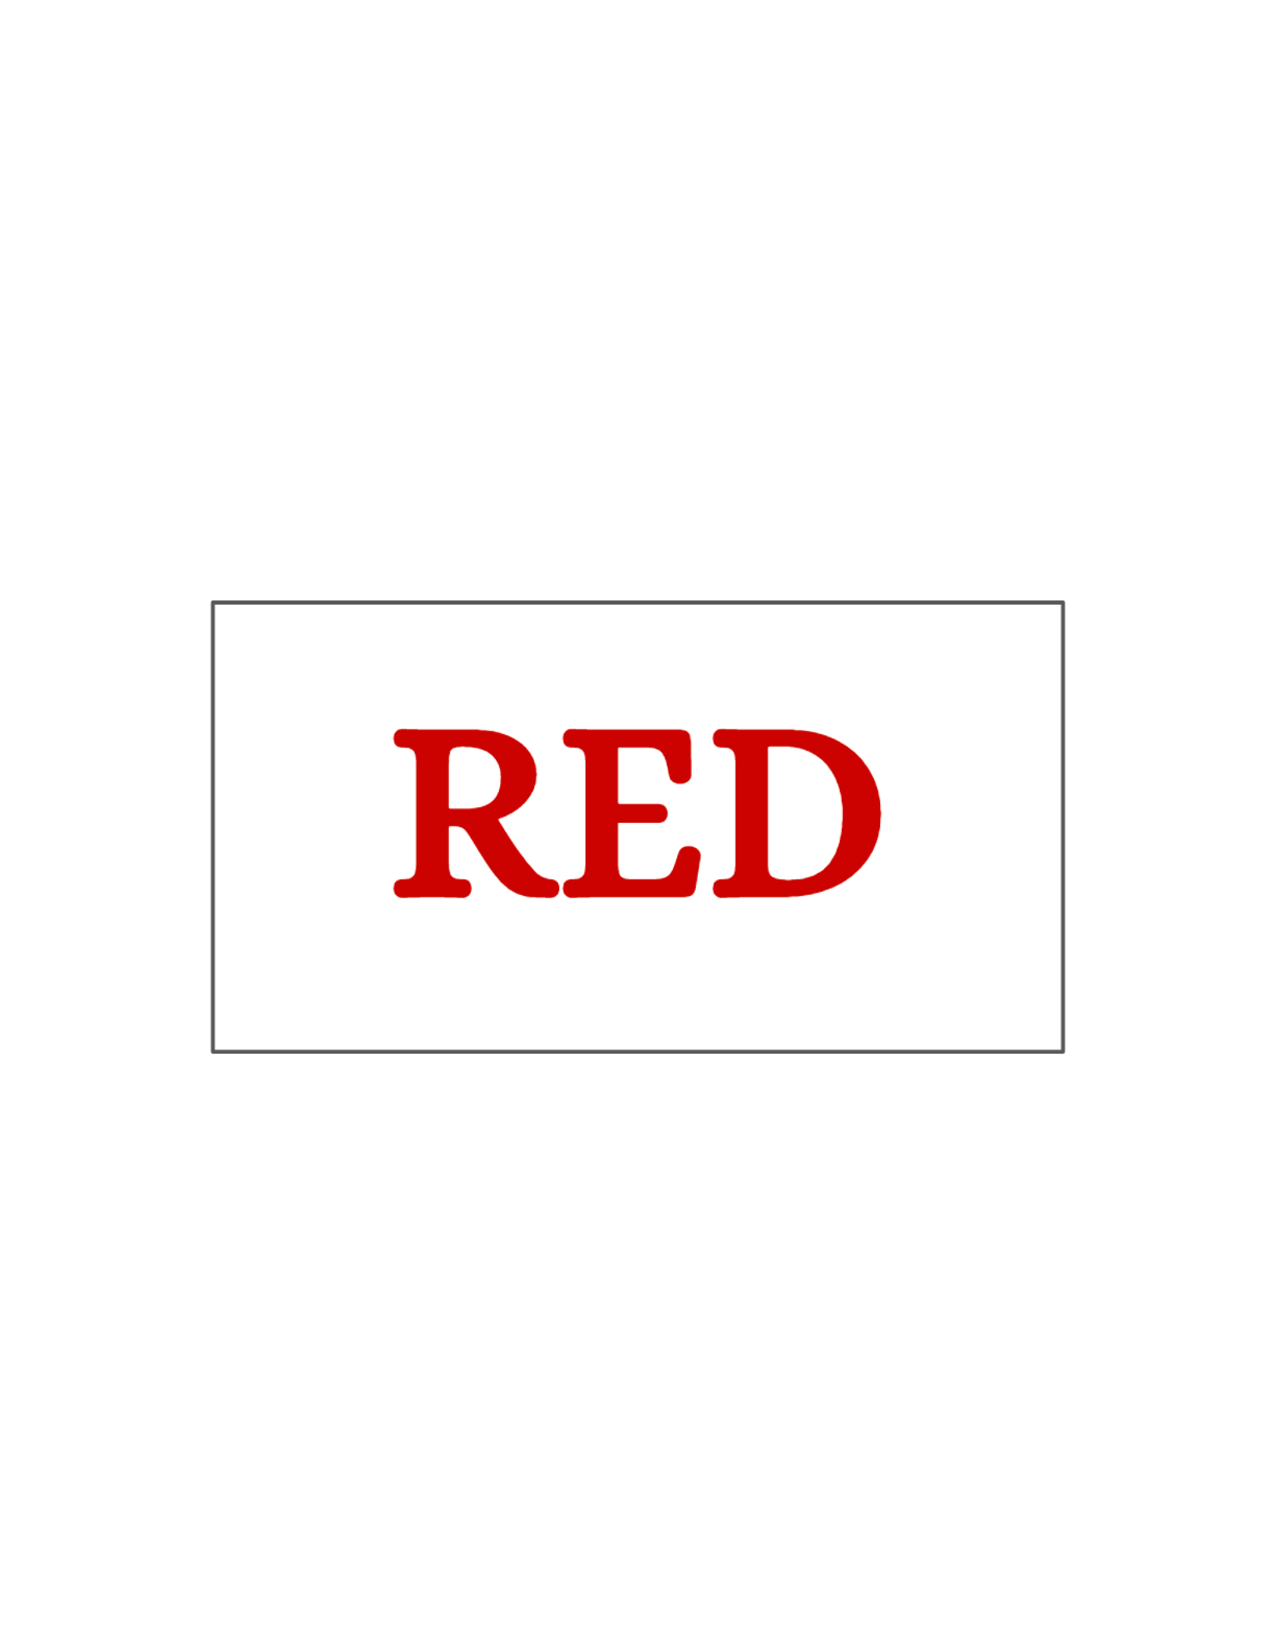
\includegraphics[width=7cm]{fig_red_in_red} }}%
  %  \qquad
    \subfloat[An incongruent Stroop stimulus.]{{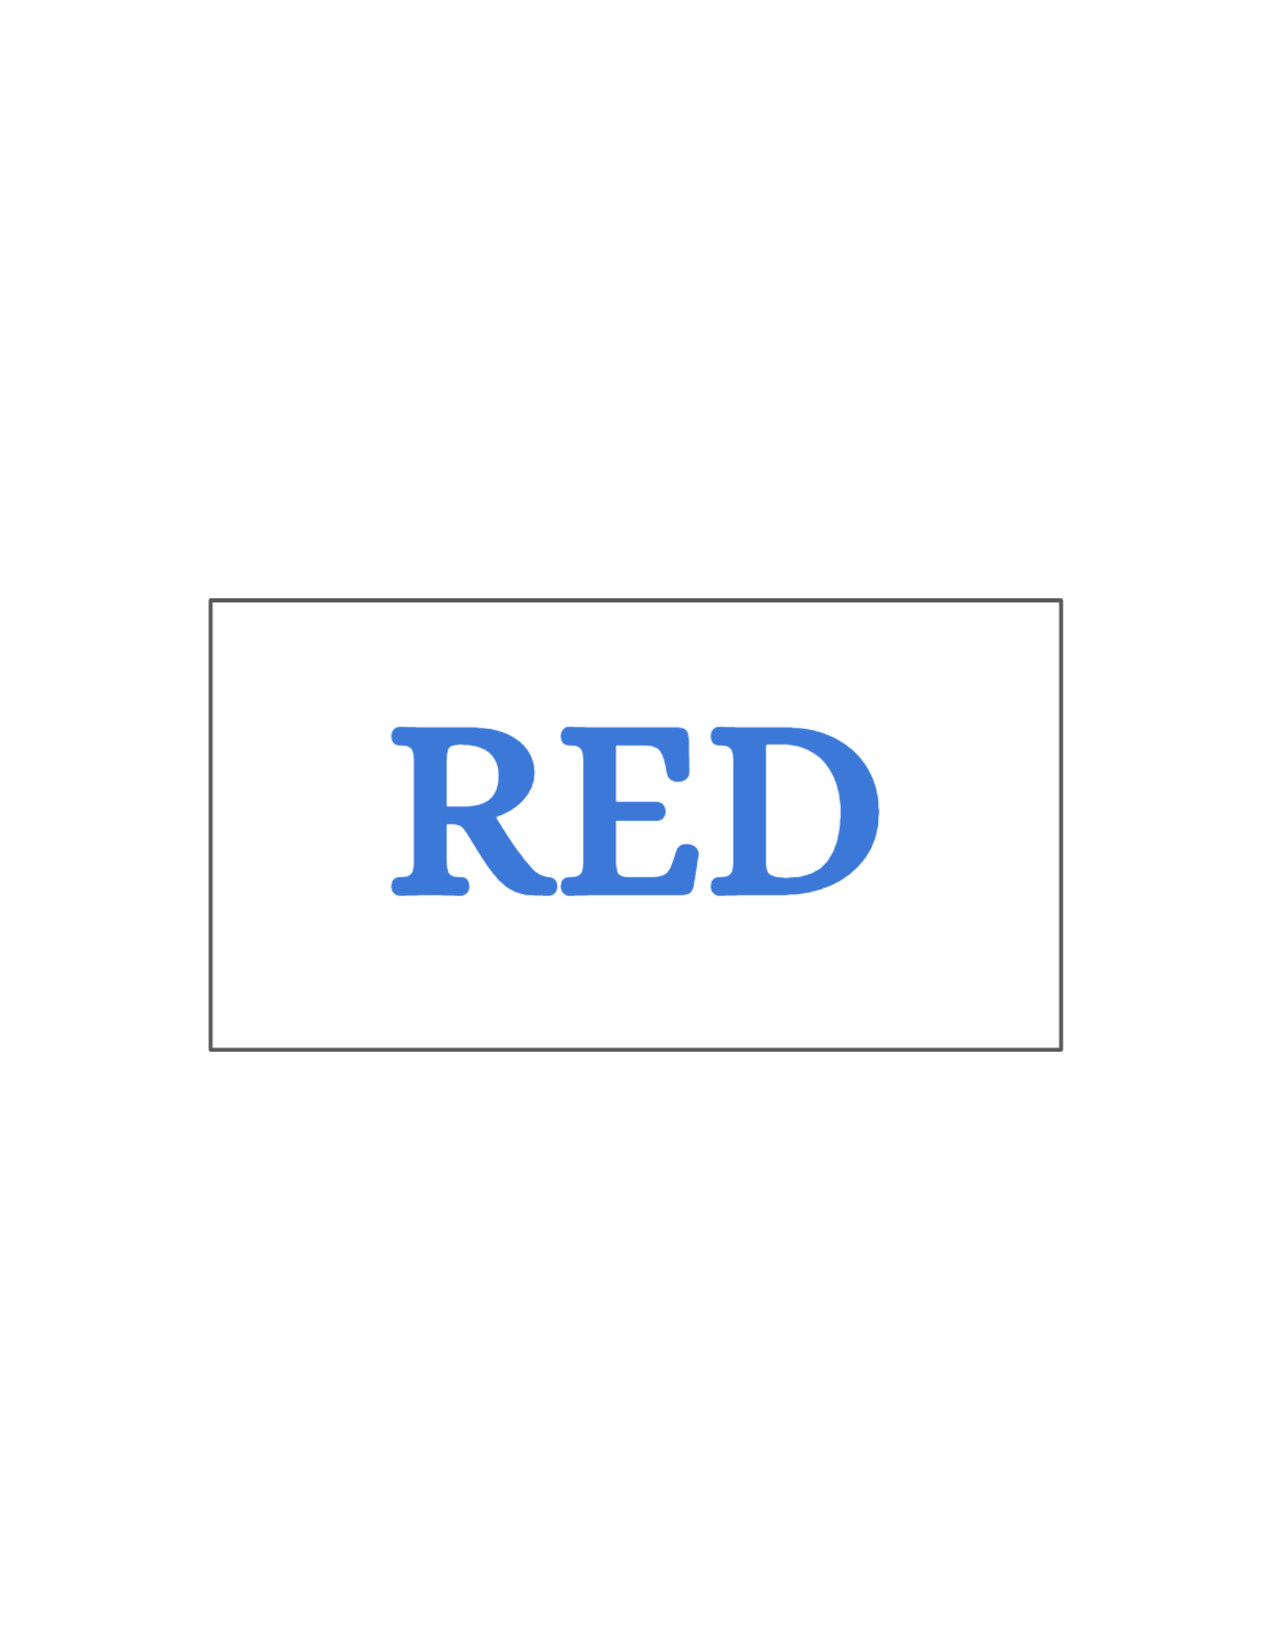
\includegraphics[width=7cm]{fig_red_in_blue} }}%
    \caption{Example Stroop stimuli.}%
    \label{fig:stroop_example}%
\end{figure}


\begin{figure}[t]%
    \centering
    \subfloat[The full crossing of possible stimuli.]{{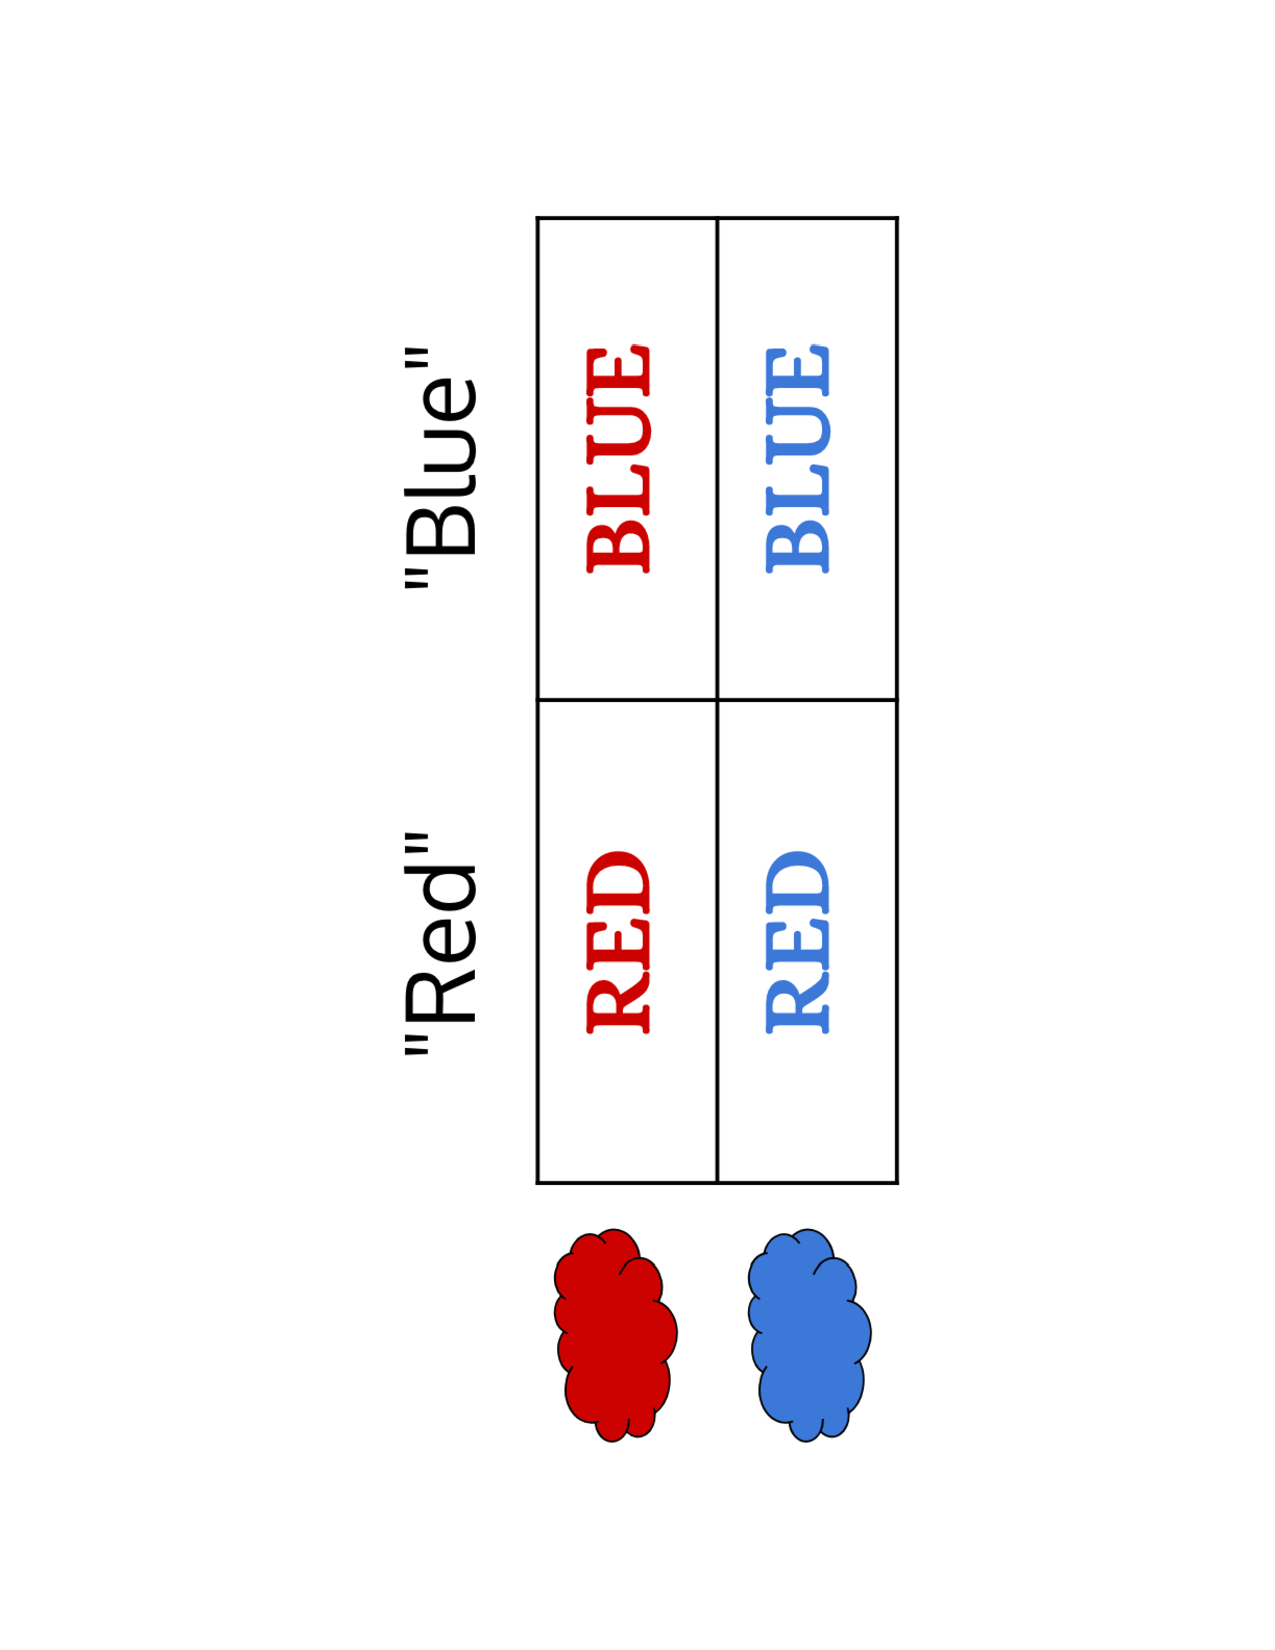
\includegraphics[angle=270,origin=c,width=8cm]{fig_simple_full_crossing}}}%
  %  \qquad
    \subfloat[A possible ordering of stimuli.]{{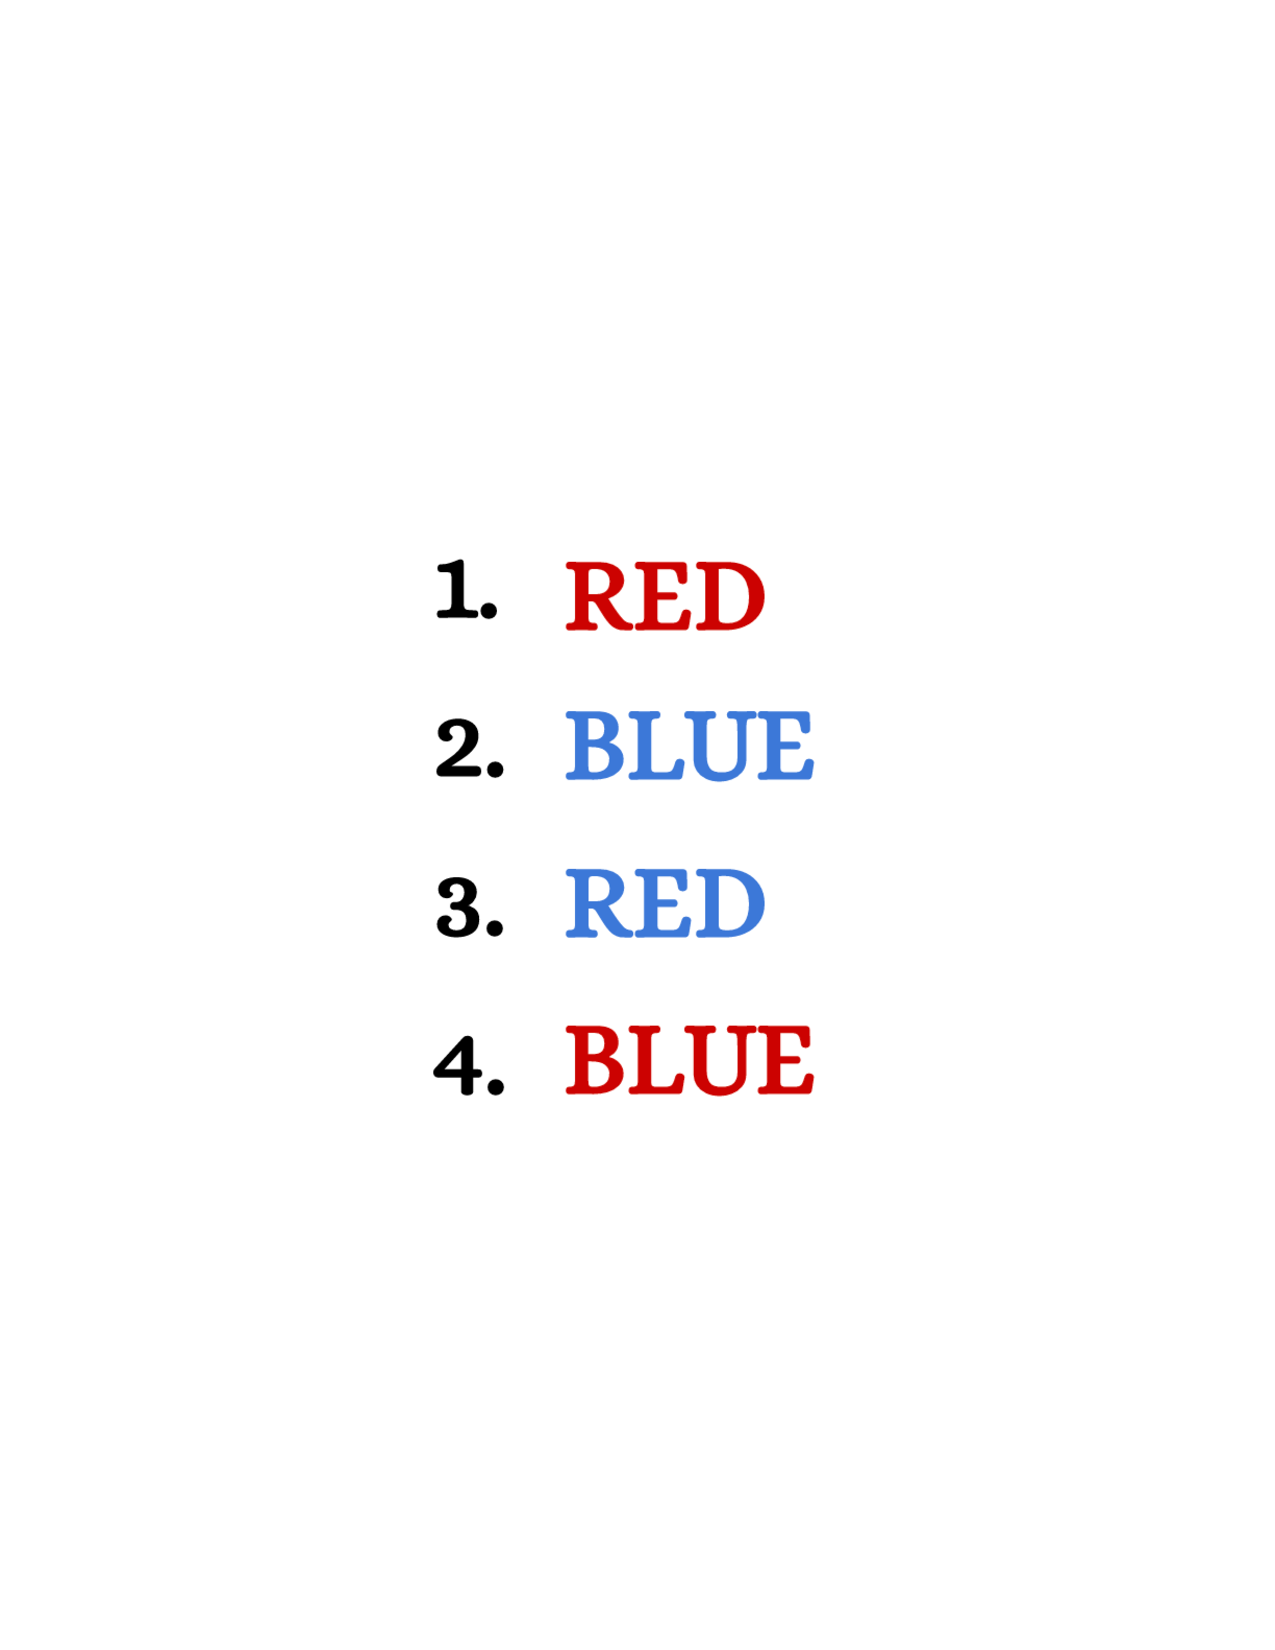
\includegraphics[width=7cm]{fig_possible_ord} }}%
    \caption{All stimuli and a possible ordering.}%
    \label{fig:simple_full_crossing}%
\end{figure}



\begin{figure}[t]
    \centerline{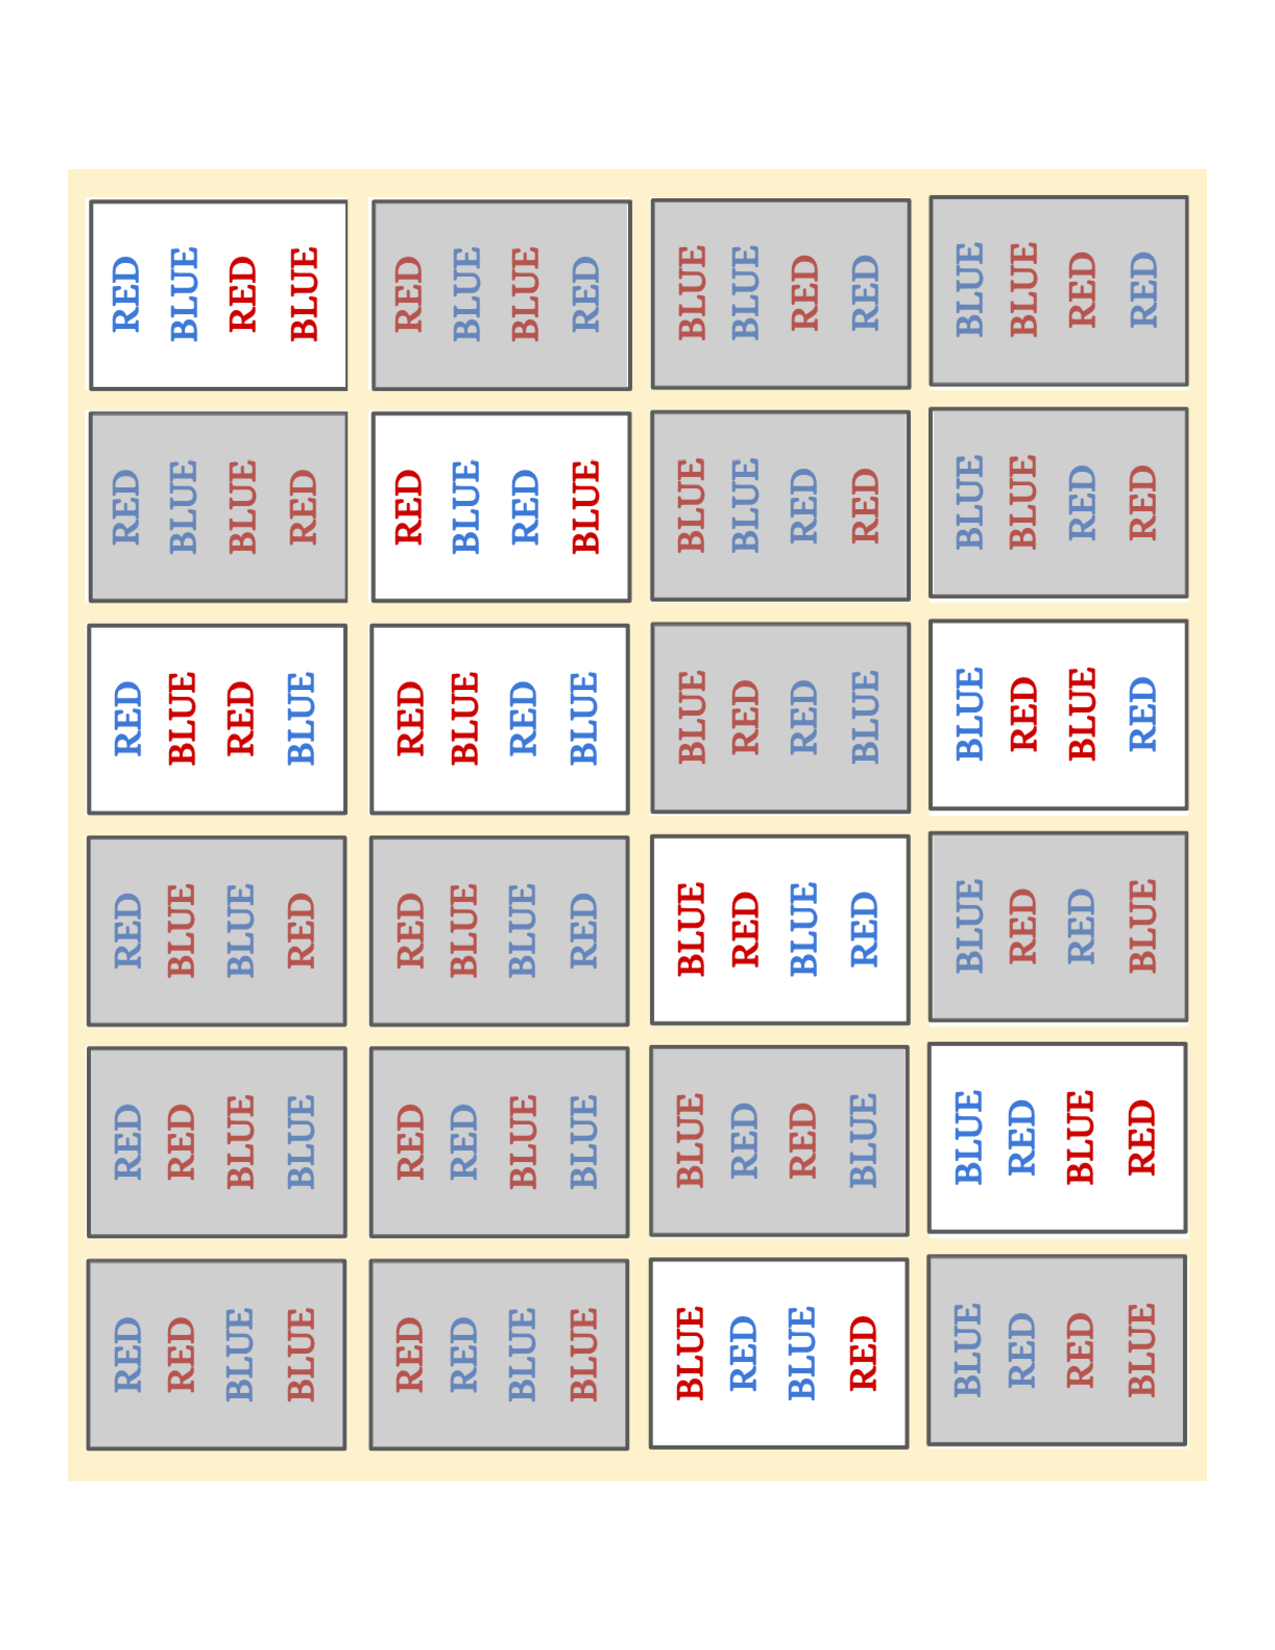
\includegraphics[angle=270,origin=c,width=10cm]{fig_valid_seqs}}
    \caption{Of the 24 possible orderings, the highlighted 8 satisfy the constraints.}%
    \label{fig:valid_seqs}%
\end{figure}


\section{A Language for Experimental Design}

Let's see how the simple Stroop experiment can be represented in SweetPea, and then at how that representation can be translated to a boolean formula to generate an experimental sequence.

The version of the SweetPea language we'll discuss is embedded in Python, so uses Python syntax.

First, we represent the factors directly as a list of levels:

%\begin{code}
\begin{verbatim}
ink_color = ("ink_color", ["red", "blue"])
text      = ("text",      ["red", "blue"])
\end{verbatim}
%\end{code}

Next, let's represent the constraint that there should be no repetitions of stimuli whose text is the same. \begin{verbatim} NoMoreThanKInARow \end{verbatim} is a constraint constructor function in SweetPea, which allows us to declaratively specify the constraint:

\begin{verbatim}
k = 2
constraints = [NoMoreThanKInARow(k, ("text", "red")), NoMoreThanKInARow(k, ("text", "blue"))]
\end{verbatim}

Having specified the factors and the constraints over those factors, we can now specify the rest of the experimental design:

\begin{verbatim}
design = [ink_color, text]
crossing = design

experiment = full_crossing(design, crossing, constraints)

synthesize_trials(experiment)
\end{verbatim}

In this example, the design and the full crossing are the same, though that doesn't need to always be the case. We specify the experiment to be the full crossing, but more generally we can construct experiments out of multiple "blocks" of crossings. The call to synthesize\_trials translates the experiment to a boolean formula representation and calls the SAT sampler.

\section{A Runtime for Uniform Sampling}

A \emph{boolean formula} consists of \emph{boolean variables} combined using boolean operators, such as AND, OR and NOT. A \emph{satisfying assignment} is a specification of True or False to each boolean variable which causes the entire formula to evaluate to True. Some formulas are unsatisfiable.

An example of an unsatisfiable formula is (A AND (NOT A)). Regardless of whether A is True of False, this formula will always evaluate to False. In contrast, the formula (A AND B) is satisfied by the assignment A is True and B is True, because (True AND True) evaluates to True.

How do we represent the program above as a boolean formula?

First, we represent each level of each trial as a boolean variable, which corresponds to whether or not that level is chosen for the produced experimental sequence. For our Stroop example, there are 4 trials, each of which have 4 boolean variables corresponding to each of the levels for a total of 16 boolean variables. A real experiment will have on the order of hundreds to thousands of boolean variables. These level variables are bound by additional constraints such as that only one level per factor is true, as well as constraints that say how many instances of a level should exist in a given experimental block.

For our Stroop example, this means that for each trial we create boolean variables to represent ink\_color=red, ink\_color=blue, text=red, text=blue. We create boolean formulas for each trial which say that exactly one of ink\_color=red or ink\_color=blue must be true, and that there must be two ink\_color=red's in the fully crossed block.

We have multiple strategies for encoding constraints, but for now let's say we have a strategy for encoding constraints of the form "no more than K in a row". We can use this to encode our constraint that there should be no repetitions of stimuli whose text is the same.

Once we've created this boolean formula which represents all the relationships which the levels must fulfill, we can pass this formula to the SAT sampler. If there exists an assignment of the boolean variables which satisfies all the constraints, the sampler will return one such assignment. If there are no satisfying assignments the sampler will state that the formula is unsatisfiable.

The solution that the sampler finds is guaranteed to be approximately uniformly probable in the space of all possible solutions. We currently use the SAT sampler Unigen, but providing this guarantee is the goal of all uniform sampling. The sampler provides this goal by using a special family of hash functions called universal hash functions. For our Stroop example, this means that each of the 8 valid orderings in \figref{valid_seqs} should be approximately equally likely.

If the sampler finds a satisfying assignment to the variables, we can then translate those variables back to the levels they represent. For our Stroop example, this means we will get assignments to the 16 boolean variables, 4 of them for each trial. These will determine the values of each of the trials, and because we have satisfied all the necessary constraints, results in a valid ordering of the trials.

We'll revisit this example in Chapter 7 to see an end-to-end encoding of the Stroop experiment, as well as the sequences produced by SweetPea.

%%% -*-LaTeX-*-

\chapter{SweetPea Language}

SweetPea achieves its goal of creating unbiased experimental sequences from high-level experimental designs by relying on a SAT sampler. Writing experimental designs in the language of a SAT sampler-- that is, as a boolean formula-- is highly uncomfortable. SweetPea, therefore, conviniently bridges the gap between scientists and SAT samplers: scientists describe their experimental designs in the terms they usually use in their domain, and SweetPea translates that high-level specification into an enormous low-level boolean formula. The SweetPea runtime then passes the SAT sampler Unigen that formula, and translates the low-level assignments into a high-level experimental sequence which satisfies the design. That experimental sequence is guaranteed to be approximately as likely as any other sequences which fulfills the design, reassuring scientists that they did not accidentally introduce bias because of the way the sequence was constructed.

In this chapter, we'll document the features of the SweetPea language. They largely follow the components we saw in the Overview chapter-- experimental designs consist of trials described in terms of factors and levels, and constraints and relationships over those trials, described here in terms of windows and derivation functions, and counting and balancing constraints. Finally, the full experiment is described in terms of a design, a crossing and experimental blocks. Here we'll look at a variety of experiments which motivate these various features, and the high-level language we provide to describe those experiments. In the next chapter we'll take a close look at how these features are efficiently encoded into a boolean formula.


\section{Components of an Experiment}

We briefly saw the parts of an experiment with the Stroop test in Chapter 2. Now let's look at the range of experiments we wish to model, and how our representations of these experiments are amenable to SAT.

\subsection{Descriptions of Stimuli}

Each component of a stimuli is represented as a \emph{factor} which can take on a disrete number of \emph{levels}. In the Stroop experiment this was represented as the ink color being red of blue, and the text color being red or blue.

Experiments typically have 2 to 7 factors with 2 to 4 levels each, resulting in roughly 50 to 200 stimuli. Often the ideal goal is to \emph{fully cross} all of the factors to produce all possible combinations of stimuli. Sometimes factors are left out of the full crossing. For example, a subject can only reliably be tested for so long before they are tired, so sometimes factors which are deemed to be irrelevant to the control variables and variables of interest are excluded from the full crossing.

Levels may be nested into sub-levels. One reason to want to do this is to apply different constraints to each of the sublevels. For instance, a color factor may have nested sublevels of light colors (like yellow and pink) and dark colors (like navy and maroon).

Sometimes researchers may want to define factors with levels sampled from a continuous distribution, for example to model a spectrum of light or sound. Sweetpea currently does not support this other than by the research manually discretizing the continoum into several discrete values. This case is particularly challenging for SweetPea because it is difficult to phrase sampling a continious distribution as a boolean formula; for more thought on how we could better support this see Future Work.

\subsection{Ordering Constraints}

Researchers must have some control over the ordering of stimuli to be able to test their hypothesis. For example, if you are testing whether the presence of a certain level effects the subject's reaction time, you need control over when that level occurs and how often it occurs in relation to other levels. More generally, you need to be able to constrain the presence or absense of relationships which you define over the levels. Since levels can be grouped into arbitrary sub-levels, you should more generally be able to specify constraints on relationships over the sub-levels.

One example of such a relationship is a transition constraint, which specifies whether each level is followed by the same level (a repetition) or a different level (a switch). A common type of transition constraint is the specification that a certain level shouldn't appear more than k-times in a row.

Another example is a congruence constraint, which specifies whether the levels of different factors are, according to a user-specified metric, complementary or conflicting. A congruence constraint for the Stroop is whether the color of the ink and the text are the same (the word "red" in red ink) or not.

Another common relationship is a balancing constraint. A pair of levels is balanced if each instance shows up the same number of times; a full crossing of all levels is a fully balanced experiment.

Constraints can also be defined in terms of other constraints. For instance, in the Stroop test one may want to balance the number of congruent and incongruent levels, or to balance the transitions between congruent and incongruent levels.

More generally, new experiments may need to define relationships between levels that other existing experiments don't have. SweetPea must have enough flexibility to allow researchers to define these new relationships.

\subsection{Experimental Design and Balancing}

Experiments which include every possible combination of levels are fully crossed designs. Fully crossings are desirable because they allow the researcher to test the full space of possible stimuli.

Sometimes, however, an experiment is either too large or too small. An experiment can be too large if it has too many elements in the full crossing because there are limits on how many tasks a subject can perform in a single session reliably. If an experiment is too large it can either be restated as a full crossing of only a subset of the factors (with the non-crossed factors being assigned at random, with uniform probability), or it can be divided across subjects or across experimental sessions. An experiment can be too small if the full crossing has too few stimuli to reliably draw conclusions. In this case, the experiment can either be multiple full crossings back-to-back, or the contents of multiple full crossings combined into a larger experimental block.

Fully-crossing a design is a form of balancing-- it is the specification that each level occurs as frequently as each other level and that each level occurs once.

Sometimes the constraint of using a full-crossing makes other types of balancing impossible because the levels are over-constrained. Consider, for instance, the Stroop test with 3 different colors instead of two: then it isn't possible to both fully-cross the design and to balance the congruent and incongruent levels. (This is because there are 3 congruent levels, and 6 incongruent levels). One possible desired outcome in this case is for SweetPea to report that an experiment is over-constrained.

Another alternative is that if balancing the congruent and incongruent levels is more important than a fully-crossed design, then we can instead create a \emph{weighted crossing} instead. In a weighted crossing we can specify that we wish to under-sample certain levels (the incongruent ones in our example) or over-sample other levels (the congruent ones). Weighted crossings also allow us to express the experiments mentioned above, where the full crossing has either too many or too few stimuli to be practical.

\subsection{Experimental Structure}

An experiment is composed of one or more experimental blocks; an experimental block is a sequence of stimuli. Experiments may be organized into blocks for several reasons: there may be prologue or epilogue blocks which set up some condition for the subject, the experiment may be designed to be run in several related sessions, or consist of several sub-experiments.

It is impossible to balance some commonly desired constraints with a single block; for instance, it is not possible to have as many "repeat" transitions as "switch" transitions in the fully-balanced Stroop experiment because there are an even number of stimuli, resulting in an odd number of transitions. This means it's not possible to have as many of one transition as the other.

There are two approaches to resolving this issue. The first is nearly-balancing the levels: instead of requiring that there are exactly the same number of each level, require that there are the same number plus-or-minus one. The other solution is to create a "throw-away" block with a single stimuli in it which is used to satisfy the transition balancing constraint without being included in the full-crossing constraint.

As mentioned in the previous section, it is also sometimes useful to have multiple blocks to repeat stimuli for an experiment with too few stimuli or to break up an experiment with too many stimuli across several sessions or subjects.

\section{SweetPea Primitives}

Now that we've seen a range of experiments that we wish to represent, let's see how we can represent them in SweetPea. Here we'll look at the high-level encodings we use, and why those encodings are amenable to being represented in SAT. In the next chapter we'll look at the SAT encodings in more detail.


\begin{verbatim}
Experiment         = Listof( Blocks )
Block              = Design Crossing Constraints
Design             = Listof( Factor )
Crossing           = Listof( Factor ) CrossingType
CrossingType       = FullyCrossed
                   | MultipleFullyCrossed
Constraint         = ExactlyKInARow K (FactorName, LevelName)
                   | AtMostKInARow  K (FactorName, LevelName)
                   | AtLeastKInARow K (FactorName, LevelName)
Factor             = FactorName Listof( LevelName )
                   | FactorName DerivedLevel
DerivedLevel       = LevelName Window
Window             = Transition          DerivationFunction
                   | WithInTrial         DerivationFunction
                   | Window Stride Width DerivationFunction
DerivationFunction = ( Listof( LevelName )... ) -> Boolean
FactorName         = <any printable type>
LevelName          = <any printable type>
\end{verbatim}




\subsection{Factors and Levels}
Factors have names, and a possibly nested list of levels, each of which also has a name. Names are used to specify the experimental sequence that the runtime eventually returns, but they do not need to be strings. They can be any "printable" data-type; this can be useful because names are referenced in user-defined constraints as we'll see in the next subsection.

\begin{verbatim}
example_factor = ("example_name", ["example_level"])
boolean_factor = ("booleans", [False, True])
text           = ("text",      ["red", "blue"])
light_colors   = ("light_colors", ["pink", "aqua"])
dark_colors    = ("dark_colors", ["navy", "maroon"])
ink_color = ("ink_color", [light_colors, dark_colors])
\end{verbatim}

In the resulting experimental sequence, exactly one choice of level is selected per trial. Internally, the experimental sequences is represented as a list of trials, where each trial is represented as a list all possible levels. There are multiple possible encodings, but the one we chose here is a "one-hot" encoding, where each level is a boolean variable which indicates whether or not it is chosen. All the boolean variables corresponding to levels of a single factor can then have an additional constraint applied that exactly one must be true. This has the effect of "chosing" one level for every factor in the trial, thereby specifying the trial. Because we do this for every trial, a satisfying assignment to these constraints represents a valid experimental sequence. See [diagram] for an example, and see Chater 6 for a more detailed discussion on the trade-offs of the choice of this, and other, encodings.

Nested levels are handled in exactly the same way- the nesting is just a way to reference a grouping in the high-level representation. This is useful because it can be used to talk about relationships between groups, ie, in constraints. At the boolean representation level, however, these groupings are irrelevant and the structure is flattened.

\begin{figure}[t]
    \centerline{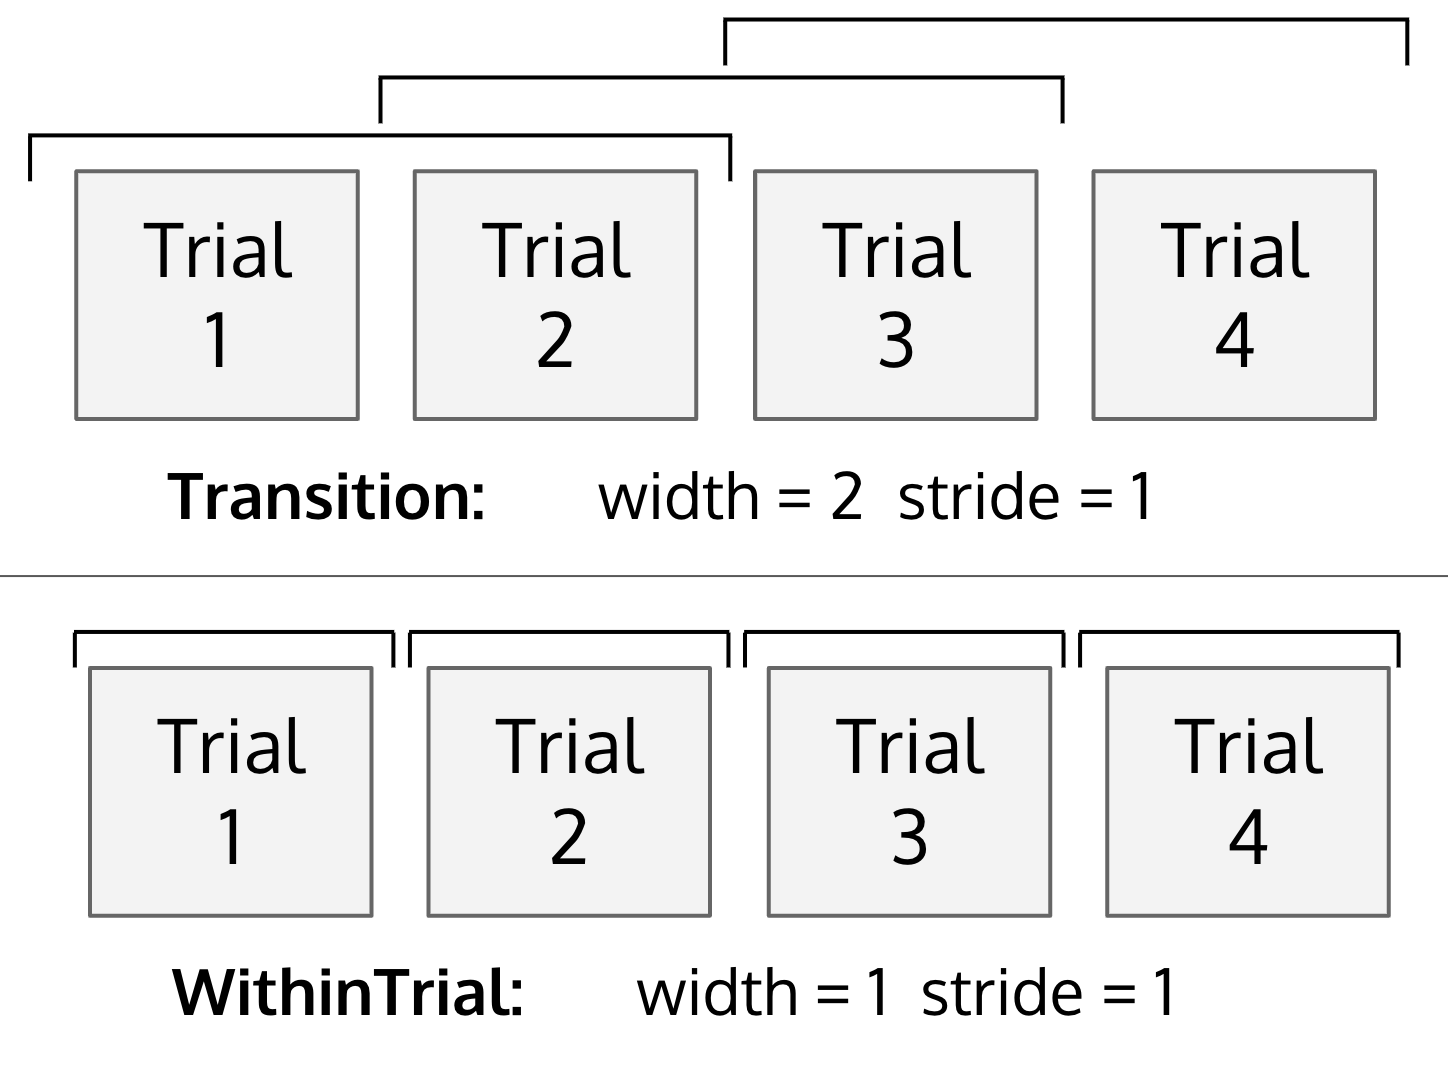
\includegraphics[origin=c,width=10cm]{fig_windows}}
    \caption{Windows define the scope of relationships between trials.}%
    \label{fig:windows}%
\end{figure}


\subsection{Deriving Levels with Windows}

How do we represent relationships between levels and enforce constraints over them? All of the constraints we are considering relate to order, so let's consider a symbolic window which slides over the list of trials. A window has a width and a stride. The width specifies how many trials to consider at once; the stride specifies how many trials to move forward by when the window moves. When combined with user-defined functions, windows allow the user to specify new "derived" levels and factors based on the values of the levels within the window. We have shorthands for two common window sizes: "WithinTrial" windows, which are used to define new properties based on properties of each individual trial, and "Transition" windows, which are used to define properties based on each consecutive pair of trials.

Consider the transition relationship, which for a given factor specifies whether each following trial has the same value for that factor (a repetition) or a different value (a switch). We will represent this relationship as a new, derived, factor. This factor has two levels: one level which indicates that the following stimuli was a repetition, the other that it was a switch. What are the parameters for the window for this relationship? Because we consider two trials at a time, and want to consider all pairs of consecutive trials, the width is two, and the stride is one.

Given this conceptual window, the user can then provide a function for each level of the derived factor which specifies, based on the values of the levels which are "in scope" in the window, whether the derived level is selected or not. For the transition example, this may look like:

\begin{verbatim}
def repetition(ink_colors):
  if ink_colors[0] == ink_colors[1]:
    return True
  return False
\end{verbatim}

The repetition function takes a list of ink colors. Because we're considering all consecutive pairs of trials, the window size is two, so the length of the ink colors list is also two. Conceptually, this function will be applied to all consecutive pairs of trials and report whether those trials are repeat or not.

We can use this repetition function to define a new pair of levels. Recall that levels act as indicators; when a level of a trial is true, that means that trial possesses the quality that level represents. The level derived using a transition-wide window and the repetition function defined above is true when the trial is has the same ink color property as the trial before it. Because levels can be defined to be any [printable] type, derivation functions can use any property of the level name as part of their logic.

Putting it all together, these derived levels are represented in SweetPea as:

\begin{verbatim}
ink_color = ("ink_color", ["red", "blue"])
text      = ("text",      ["red", "blue"])

def repetition(ink_colors):
  if ink_colors[0] == ink_colors[1]:
    return True
  return False

repeat_level  = DerivedLevel("rep", Transition(repetition, [ink_color, ink_color]))
switch_level  = DerivedLevel("swi", Transition(repetition, [ink_color, ink_color], False))
transitionFactor = Factor("congruent?", [repeat_level, switch_level])

\end{verbatim}

Let's consider another use-case. In the Stroop experiment, it is useful to ask whether or not a trial is congruent, meaning whether the ink color and the text specify the same color or not. We can define this relationship by considering a WithinTrial window, in which the width is one (since we consider a single trial at a time), and the stride is also one. The derivation function for congruence is similiar to the one for repetitions; here however we always compare the first (and only) item in the ink colors and texts lists.

\begin{verbatim}
ink_color = ("ink_color", ["red", "blue"])
text      = ("text",      ["red", "blue"])

def congruent(ink_colors, texts):
  if ink_colors[0] == text[0]:
    return True
  return False

con_level  = DerivedLevel("rep", WithinTrial(congruent, [ink_color, ink_color]))
inc_level  = DerivedLevel("swi", WithinTrial(congruent, [ink_color, ink_color], False))
congruenceFactor = Factor("congruent?", [con_level, inc_level])

\end{verbatim}

Windows allow us to represent, more generally than just transitions and within-trial constraints, relationships across a sequence of trials. See \figref{windows} for an illustration. Some experiments may wish to define relationships which skip trials in the middle of the sequences. An example is an experiment with a "bait" trial: subjects are asked to respond based on a property of a trial some number of trials previous. Additionally, changing the stride allows for things like specifying a constraint over the first half, and then second half of the experiment.

\subsection{Experimental Design, Balancing and Experimental Structure}

Once we've described the trials in terms of levels and factors, we need to specify the set of trials that make up the experiment. The design of the experiment is the specification of factors represent a trial. To specify the set of trials in the experiment we need to specify the crossing of the design. As mentioned before, a full crossing is commonly, but not always, used.

The final aspect we need to specify is the structure of the experimental sequence. An experimental sequence is a list of one or more experimental blocks. Each experiemental block consists of a crossing of the experimental design. Some experiments may wish to specify multiple experimental blocks to represent prologue or epilogue blocks, or to split an experiment across multiple sessions.

Having discussed and motivated all of the aspects of the SweetPea language, in the next chapter we'll see how these elements are encoded as a boolean formula.

%%% -*-LaTeX-*-

\chapter{SAT Encodings}

In this chapter we will examine how the language forms we saw in the previous chapter are efficiently encoded as boolean formulas. A program in SweetPea is translated to a boolean formula in Conjunctive Normal Form (CNF), which is a canonicalization that is frequently used by SAT solvers and samplers. We use two techniques for efficient SAT encodings: we encode large "counting" constraints as circuitry which counts set bits in a bitstring, and user's derivation constraints more directly. After examining how a program is encoded, we will also discuss the runtime communication with the sampler, and why the correctness guarantees are preserved.

\section{Conjunctive Normal Form (CNF)}

A boolean formula consists of boolean variables combined using boolean operators, such as \texttt{and}, \texttt{or} and \texttt{not}. There are many canonical forms for boolean formulas; the one that SAT solvers commonly use is Conjunctive Normal Form (CNF). CNF is an "and of ors". This means that CNF is built out of OR clauses, which are clauses in which the boolean OR operator is applied to a list of variables. \texttt{A or B or (not C) or D} is an example of an OR clause. CNF is then the AND operator applied to a list of OR clauses. \texttt{(A or B) and (C or not D)} is an example of a boolean formula in CNF.

SAT solvers typically process boolean formulas in CNF. This is partially because they are amenable to the search strategies that solvers commonly employ while searching for satisfying assignments, and partially because there is an efficient translation from a boolean formula in any form to the CNF canonical form.

More specifically, solvers typically process boolean formulas in the DIMACS CNF form. In the DIMACS convention, boolean variables are denoted by their index, and negation is denoted by a minus sign. This means that a formula like \texttt{(A or B) and (C or not D)} is represented as \texttt{(1 or 2) and (3 or -4)}. This index based renaming is very convenient as a convention for generating fresh variable names-- we just need to increment the variable counter to get a fresh variable. Each or-clause is written on an individual line, and every term within the or-clause is written as an element of a list; each list is terminated with the number 0. Finally, each formula also has a header which clues the consumer to the number of variables and clauses in formula. The full DIMACS CNF specification of the example in this paragraph is:


\begin{verbatim}
p cnf 4 2
1, 2, 0
3, -4, 0
\end{verbatim}


This specification is the language required to leverage the awesome power of SAT samplers and solvers, but it is clearly not amenable to being manually specified by human hands for anything but the most toy examples. That is why SweetPea provides a high-level domain-specific interface which compiles to these low-level specifications. An interesting aspect of the translation is ensuring that the encoding is efficient: that is, polynomial in the number of number of variables and clauses with respect to the constraint size.

\section{Representing SweetPea Primitives in CNF}

Recall that experimental designs describe trials in terms of factors and levels, and the relationships between those trials in terms of windows, derivation functions and counting constraints. Here, let us see how all of those components are encoded into a boolean formula; in the next chapter we will discuss trade-offs of some encoding decisions and more details.

\subsection{Representing Levels and Necessary Constraints}

% \begin{figure}[t]
%     \centerline{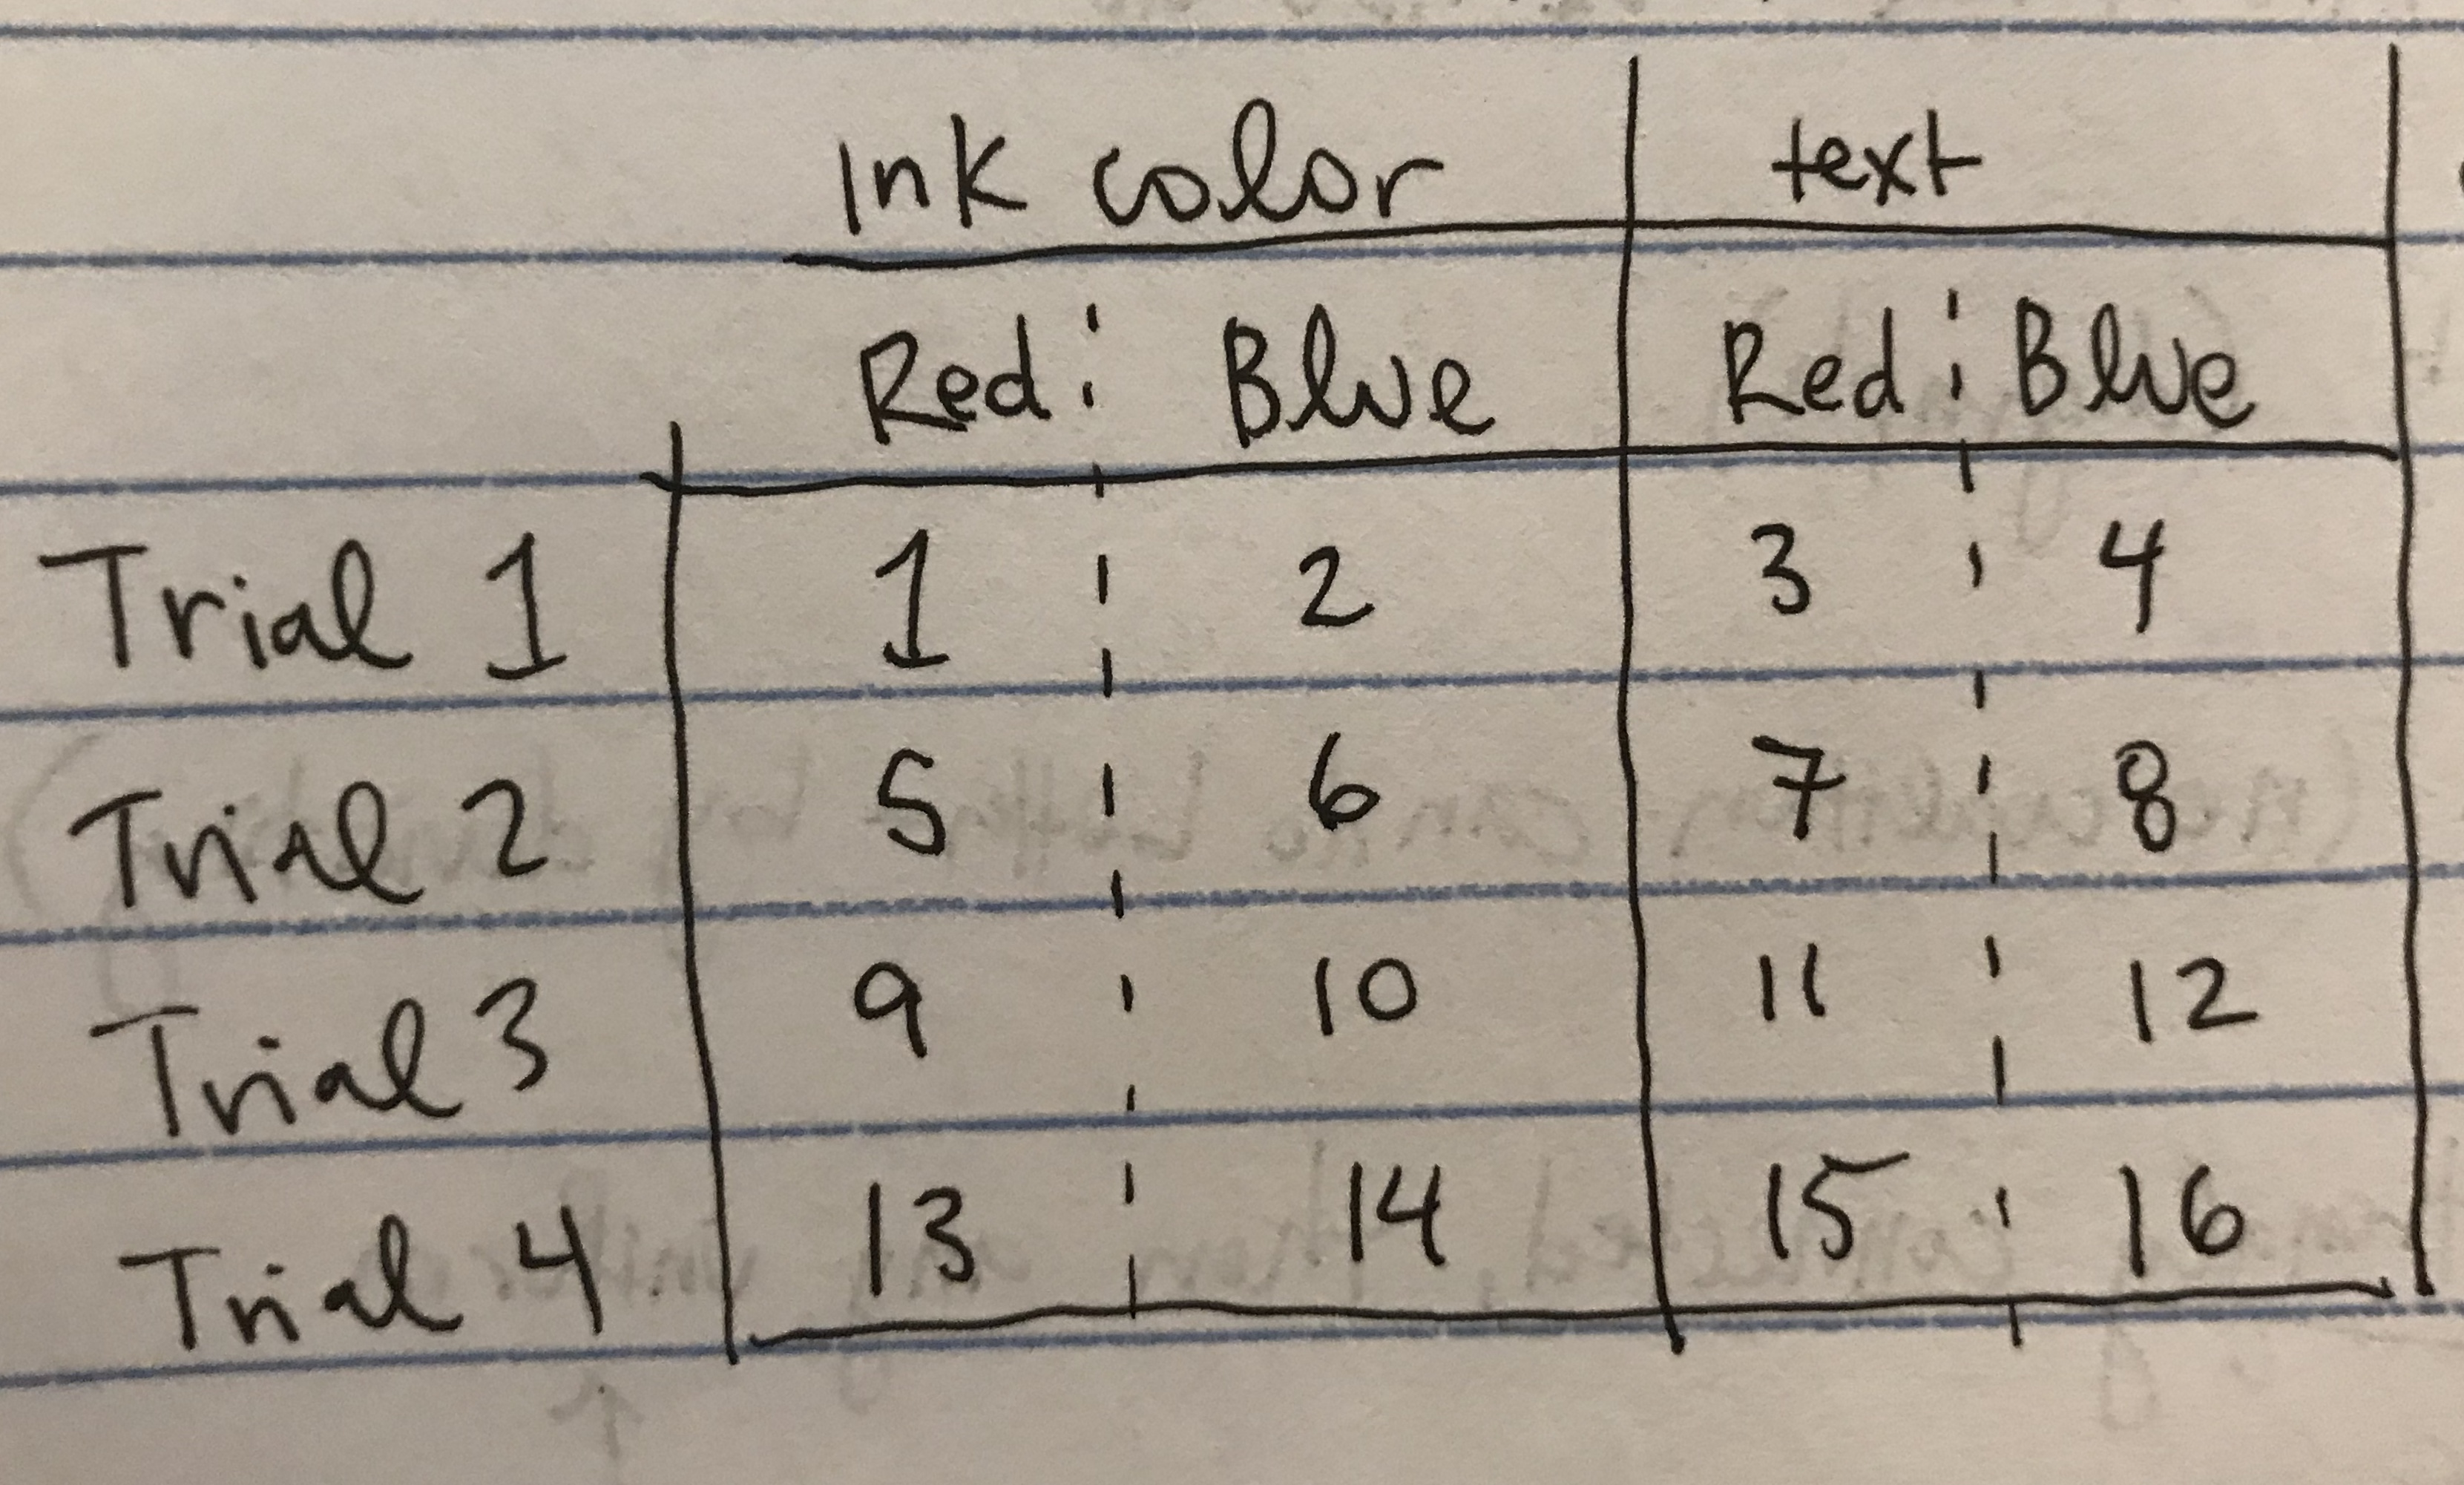
\includegraphics[origin=c,width=10cm]{encoding_strupe_vars}}
%     \caption{Variable allocation for the running Stroop example.}%
%     \label{fig:encoding_strupe_vars}%
% \end{figure}




An experimental sequence consists of a specification for every trial in the experiment. Each trial is parameterized by factors, and the specification indicates which level of each factor is selected. Levels correspond naturally to boolean variables; a factor has one level at a time selected and each level can exist in either a selected state or a non-selected state.

The encoding we use allocates one boolean variable for each level of each factor of each trial. See figure \tabref{encoding_strupe_vars} for a visualization of the variable allocation for the running Stroop example. In the running example, there are 4 trials, each of which is described by two factors with two levels. The encoding we use allocates one variable for every factor for every trial. As mentioned in the previous subsection, variables in the DIMACS CNF format are index-based, which means that the number 1 refers to the first boolean variable and so on. This means that the assignments to variables 1 through 4 represents the specification of the first trial. For instance, the assignment \texttt{1 -2 -3 4} means the display color is red (and not blue), and the text is blue (and not red). For any experiment we allocate (total number of levels) * (number of trials) boolean variables which directly encode a specification of an experimental sequence.





% \begin{figure}[t]
%     \centerline{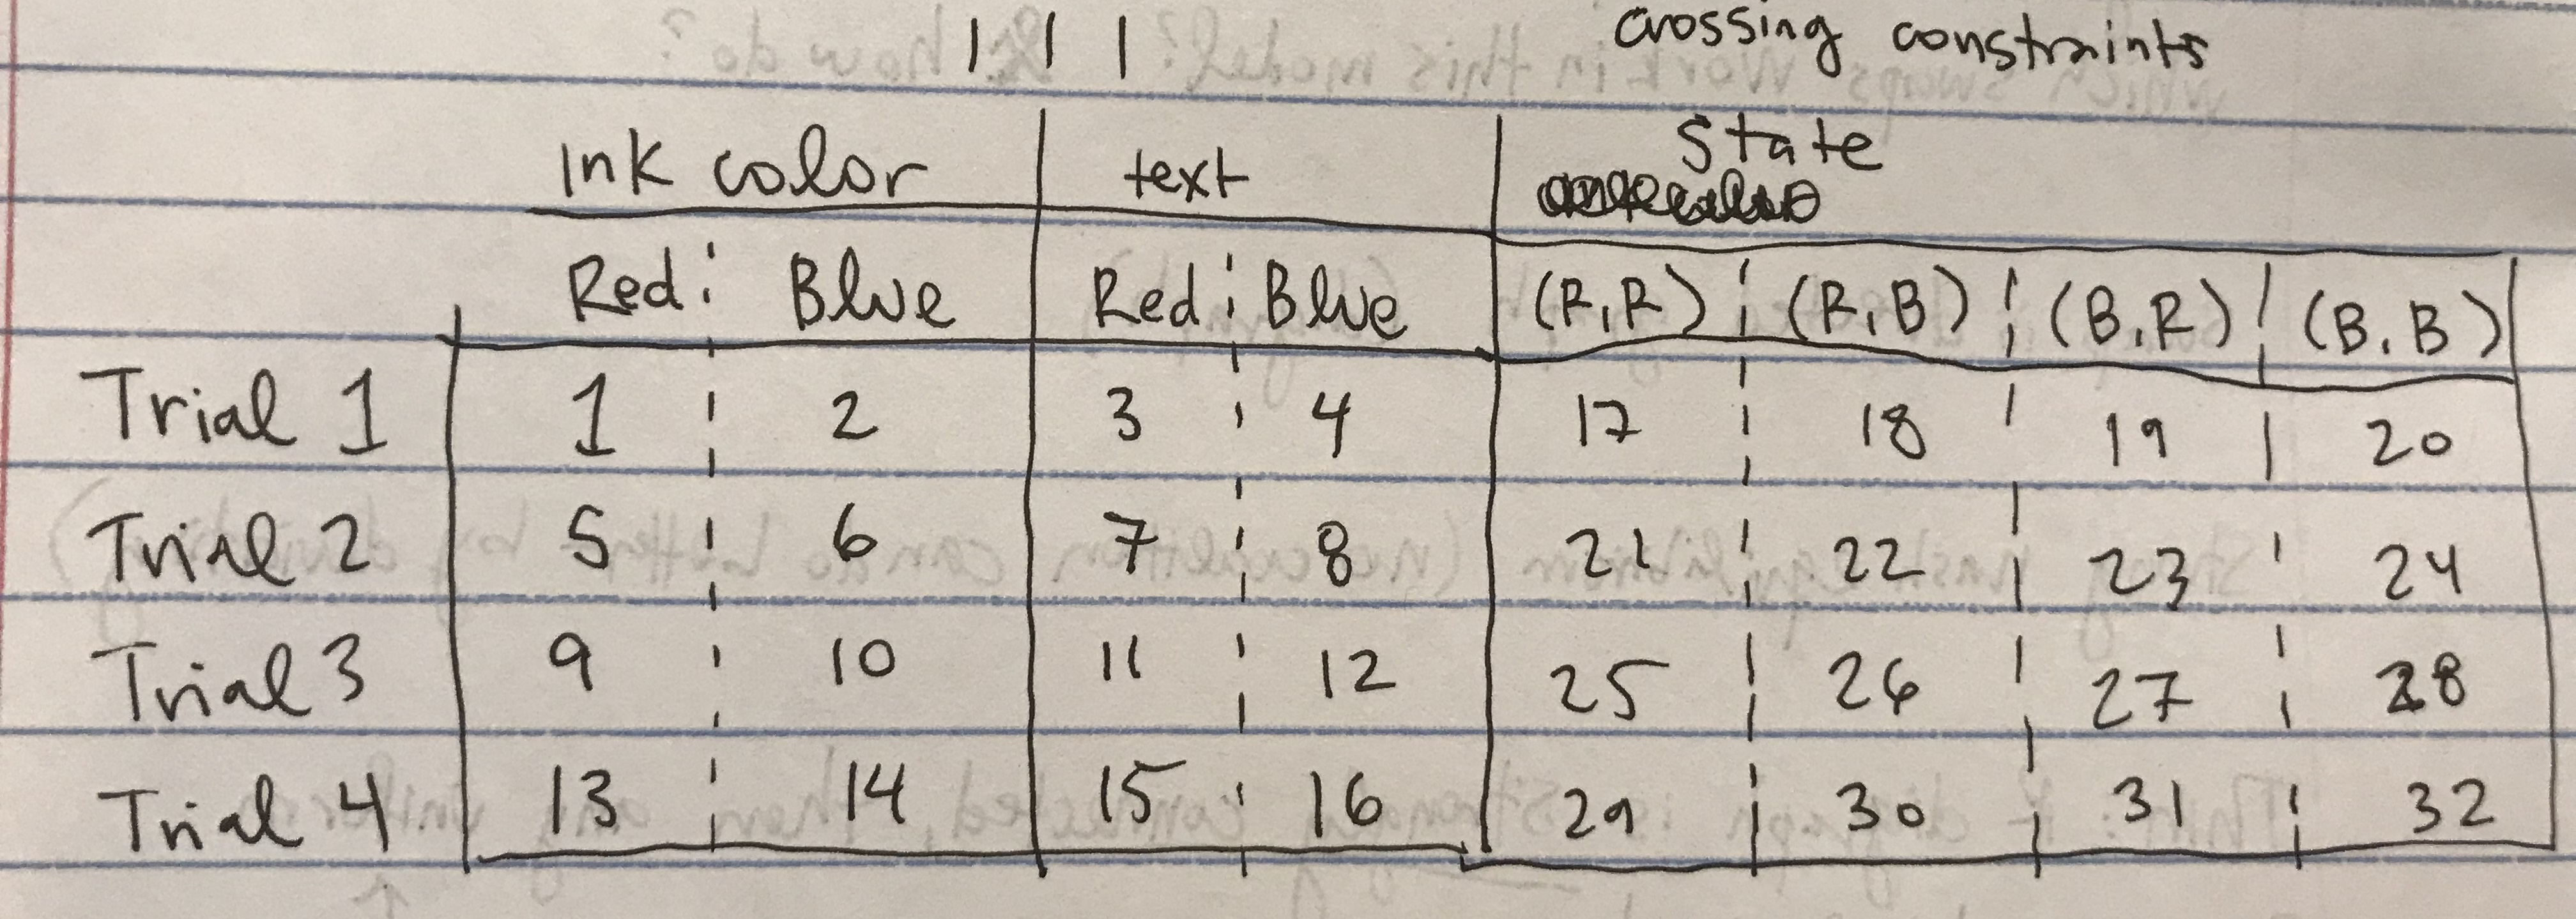
\includegraphics[origin=c,width=10cm]{stroop_crossing_vars}}
%     \caption{Additional variable allocation necessary for encoding the states possible in the full crossing.}%
%     \label{fig:stroop_crossing_vars}%
% \end{figure}

There are two kinds of constraints which need to be encoded; user-defined constraints and two other constraints which are always necessary to correctly model the experiment. The first are \emph{consistency constraints} which state that only one level of each factor is selected at once. In the running example constraints of the form \texttt{(1 and not 2) or (not 1 and 2)} for each pair of levels would ensure that only one level is true at a time. The second kind of constraint is a \emph{crossing constraint} which ensures that the correct number of each kind of possible trial occurs in the experimental sequences.

Representing crossing constraints is more complicated. In the running example, the logic for the crossing constraints should ensure that there is one (red display, red text), one (red display, blue text), one (blue display, red text) and one (blue display, blue text). To do encode this, we allocate 4 more variables for each trial, each of which literally encodes which of those 4 states that trial represents. See figure \tabref{stroop_crossing_vars} for a visualization of the additional variables. Let us look at the constraints we need to add for the first trial-- first we will add a constraint that specifies that trial is in the (red display, red text) state if-and-only-if the red display level is selected, and the red text level is selected \texttt{(17 iff (1 and 3))}. We add constraints of this form for the other 3 states as well, ie \texttt{(18 iff (1 and 4))}, \texttt{(19 iff (2 and 3))}, \texttt{(20 iff (2 and 4))}. Next, we create constraints to ensure that exactly one of each of the state variables across all the trials is true, ie, (exactly one of 17, 21, 25, 29 is true), (exactly one of 18, 22, 26, 30 is true), and so on.

A realistic experiment may have on the order of 100 trials. This means that we need to be careful with this last constraint, that exactly one of \texttt{<}list of length 100\texttt{>}, is true. In other types of crossings (see chapter 4, section 4.2.3) that constraint may more generally be exactly k of \texttt{<}list of length 100\texttt{>} is true. The naive encoding (these k, or those k, or those k, and so on) is exponential, therefore not efficient, and in practice too large for our problem size. Instead, we efficiently encode these \emph{counting constraints} following a technique similar to the one described in \cite{sinz2005towards}. For a detailed description of this algorithm, see the next chapter.

In summary, an experimental sequence is represented as a list of boolean variables for each level of each trial. Assignments to these variables uniquely specify the experimental sequence. Irregardless of other user constraints, these variables are bound by constraints to ensure exactly one level is selected at a time for each factor, and that each state in the crossing is represented the correct number of times. The next chapter will examine the trade-offs from our encoding decisions. Next we will see how these variables which represent levels can be used to encode derived levels and used with window constraints.

\subsection{Representing Derived Levels and Derivation Functions}

The current SweetPea implementation special-cases the constraint encoding for congruency and transitions because these are common constraints in the experiments we wish to model.

Let us consider a congruency derivation over the simple Stroop example. In addition to the variables which represent the levels of each trial, we will allocate 2 new variables for each trial each of which indicates whether or not the trial is congruent. This means the variable allocation looks like:

% \begin{verbatim}
% ----------------------------------------------
% |   Trial |  color   |   text   | congruent? |
% |       # | red blue | red blue |  con  inc  |
% ----------------------------------------------
% |       1 |  1   2   |  3   4   |   5    6   |
% |       2 |  7   8   |  9   10  |  11    12  |
% |       3 | 13   14  | 15   16  |  17    18  |
% |       4 | 19   20  | 21   22  |  23    24  |
% ----------------------------------------------
% \end{verbatim}





Then, we encode constraints on when these new variables are true. When is the first trial congruent? The first trial (\texttt{5}) is congruent if-and-only-if either the trial's color is red (\texttt{1}) and the text is red (\texttt{3}), or the color is blue (\texttt{2}) and the text is blue (\texttt{2}). In boolean logic this is: \texttt{5 iff (1 and 3) or (2 and 4)}. We create constraints of this form for all the remaining variables, and translate this constraint to CNF through a general CNF conversion technique.

What if instead we considered transitions? Let us reinterpret the variable named \texttt{5} to indicate whether that trial has the same text as the following trial:

% \begin{verbatim}
% ----------------------------------------------
% |   Trial |  color   |   text   | transition |
% |       # | red blue | red blue |  swi  rep  |
% ----------------------------------------------
% |       1 |  1   2   |  3   4   |   5    6   |
% |       2 |  7   8   |  9   10  |  11    12  |
% |       3 | 13   14  | 15   16  |  17    18  |
% |       4 | 19   20  | 21   22  |  23    24  |
% ----------------------------------------------
% \end{verbatim}




We can then state that the trial switches (\texttt{5}) if-and-only-if this trial's text is red (\texttt{3}) and the next trial's text is also red (\texttt{9}), or they are both blue (\texttt{4} and \texttt{10}). In boolean logic this is: \texttt{5 iff (3 and 9) or (4 and 10)}. This identical clause structure allows us to model both of these common derivations. Encoding arbitrary derivations is left as future work.

\section{Correctness Guarantees}

The goal of SweetPea is to produce experimental sequences which satisfy the experimental design with uniform probability: not favoring any valid sequence over any other. SweetPea achieves this goal by relying on the uniform samping guarantee that Unigen provides in \cite{chakraborty2013scalable}.

Unigen is a near-uniform SAT sampler. Near-uniform is defined in \cite{meel2016constrained} as

\begin{align*}
  \frac{1}{\text{number of solutions}\times(1+ \epsilon)} & \leq \text{Probability[Finding a given solution]} \\
  &\leq (1+\epsilon) / \text{number of solutions}
\end{align*}

This guarantees that the number of \emph{SAT witnesses}, or satisfying solutions, to the CNF is approximately uniformly probable. How does the number of satisfying SAT solutions relate to the number of experimental sequences which satisfy the experimental design?

When we translate from the high level specification to the boolean formula, we introduce new internal boolean variables (ie the sum and carry bits of the adders in the popcount encoding). We hypothesize that the number of satisfying SAT solutions is exactly the same as the number of experiment sequences when none of the internal boolean variables are redundant. Then, all the variables which directly encode the experiment are in lockstep with all the extra internal variables. If there are redundant variables, they could skew the number of satisfying assignments such that finding an assignment would be uniform with those variables, but not in the variables we care about. To the best of our knowledge, our encoding does not introduce redundant variables, and therefore preserves this guarantee.



\begin{table}
  \centering
  \caption{Variable allocation for the running Stroop example.}
\begin{tabular}{c|
>{\columncolor[HTML]{EFEFEF}}c |
>{\columncolor[HTML]{EFEFEF}}c |c|c|}
\cline{2-5}
& \multicolumn{2}{c|}{\cellcolor[HTML]{EFEFEF}{\color[HTML]{333333} display color}} & \multicolumn{2}{c|}{text} \\ \cline{2-5}
\multirow{-2}{*}{}            & {\color[HTML]{333333} red}              & {\color[HTML]{333333} blue}             & red         & blue        \\ \hline
\multicolumn{1}{|c|}{Trial 1} & {\color[HTML]{333333} 1}                & {\color[HTML]{333333} 2}                & 3           & 4           \\ \hline
\multicolumn{1}{|c|}{Trial 2} & {\color[HTML]{333333} 5}                & {\color[HTML]{333333} 6}                & 7           & 8           \\ \hline
\multicolumn{1}{|c|}{Trial 3} & {\color[HTML]{333333} 9}                & {\color[HTML]{333333} 10}               & 11          & 12          \\ \hline
\multicolumn{1}{|c|}{Trial 4} & {\color[HTML]{333333} 13}               & {\color[HTML]{333333} 14}               & 15          & 16          \\ \hline
\end{tabular}
\label{tab:encoding_strupe_vars}%
\end{table}


\begin{table}
  \centering
  \caption{Additional variable allocation necessary for encoding the states possible in the full crossing.}%
\begin{tabular}{c|
>{\columncolor[HTML]{EFEFEF}}c |
>{\columncolor[HTML]{EFEFEF}}c |c|c|
>{\columncolor[HTML]{EFEFEF}}c |
>{\columncolor[HTML]{EFEFEF}}c |
>{\columncolor[HTML]{EFEFEF}}c |
>{\columncolor[HTML]{EFEFEF}}c |}
\cline{2-9}
                              & \multicolumn{2}{c|}{\cellcolor[HTML]{EFEFEF}{\color[HTML]{333333} display color}} & \multicolumn{2}{c|}{text} & \multicolumn{4}{c|}{\cellcolor[HTML]{EFEFEF}state} \\ \cline{2-9}
\multirow{-2}{*}{}            & {\color[HTML]{333333} red}              & {\color[HTML]{333333} blue}             & red         & blue        & (r, r)      & (r, b)     & (b, r)     & (b, b)     \\ \hline
\multicolumn{1}{|c|}{Trial 1} & {\color[HTML]{333333} 1}                & {\color[HTML]{333333} 2}                & 3           & 4           & 17          & 18         & 19         & 20         \\ \hline
\multicolumn{1}{|c|}{Trial 2} & {\color[HTML]{333333} 5}                & {\color[HTML]{333333} 6}                & 7           & 8           & 21          & 22         & 23         & 24         \\ \hline
\multicolumn{1}{|c|}{Trial 3} & {\color[HTML]{333333} 9}                & {\color[HTML]{333333} 10}               & 11          & 12          & 25          & 26         & 27         & 28         \\ \hline
\multicolumn{1}{|c|}{Trial 4} & {\color[HTML]{333333} 13}               & {\color[HTML]{333333} 14}               & 15          & 16          & 29          & 30         & 31         & 32         \\ \hline
\end{tabular}


\label{tab:stroop_crossing_vars}
\end{table}



\begin{table}
  \centering
  \caption{Variable allocation necessary for the congruency contraint.}%
\begin{tabular}{c|
>{\columncolor[HTML]{EFEFEF}}c |
>{\columncolor[HTML]{EFEFEF}}c |c|c|
>{\columncolor[HTML]{EFEFEF}}c |
>{\columncolor[HTML]{EFEFEF}}c |}
\cline{2-7}
                              & \multicolumn{2}{c|}{\cellcolor[HTML]{EFEFEF}{\color[HTML]{333333} display color}} & \multicolumn{2}{c|}{text} & \multicolumn{2}{c|}{\cellcolor[HTML]{EFEFEF}congruent?} \\ \cline{2-7}
\multirow{-2}{*}{}            & {\color[HTML]{333333} red}              & {\color[HTML]{333333} blue}             & red         & blue        & con                        & inc                        \\ \hline
\multicolumn{1}{|c|}{Trial 1} & {\color[HTML]{333333} 1}                & {\color[HTML]{333333} 2}                & 3           & 4           & 5                          & 6                          \\ \hline
\multicolumn{1}{|c|}{Trial 2} & {\color[HTML]{333333} 7}                & {\color[HTML]{333333} 8}                & 9           & 10          & 11                         & 12                         \\ \hline
\multicolumn{1}{|c|}{Trial 3} & {\color[HTML]{333333} 13}               & {\color[HTML]{333333} 14}               & 15          & 16          & 17                         & 18                         \\ \hline
\multicolumn{1}{|c|}{Trial 4} & {\color[HTML]{333333} 19}               & {\color[HTML]{333333} 20}               & 21          & 22          & 23                         & 24                         \\ \hline
\end{tabular}


\label{tab:stroop_congruency_vars}
\end{table}



\begin{table}
  \caption{Variable allocation necessary for the transition contraint.}%
  \centering
\begin{tabular}{c|
>{\columncolor[HTML]{EFEFEF}}c |
>{\columncolor[HTML]{EFEFEF}}c |c|c|
>{\columncolor[HTML]{EFEFEF}}c |
>{\columncolor[HTML]{EFEFEF}}c |}
\cline{2-7}
                              & \multicolumn{2}{c|}{\cellcolor[HTML]{EFEFEF}{\color[HTML]{333333} display color}} & \multicolumn{2}{c|}{text} & \multicolumn{2}{c|}{\cellcolor[HTML]{EFEFEF}transition} \\ \cline{2-7}
\multirow{-2}{*}{}            & {\color[HTML]{333333} red}              & {\color[HTML]{333333} blue}             & red         & blue        & switch                     & repeat                     \\ \hline
\multicolumn{1}{|c|}{Trial 1} & {\color[HTML]{333333} 1}                & {\color[HTML]{333333} 2}                & 3           & 4           & 5                          & 6                          \\ \hline
\multicolumn{1}{|c|}{Trial 2} & {\color[HTML]{333333} 7}                & {\color[HTML]{333333} 8}                & 9           & 10          & 11                         & 12                         \\ \hline
\multicolumn{1}{|c|}{Trial 3} & {\color[HTML]{333333} 13}               & {\color[HTML]{333333} 14}               & 15          & 16          & 17                         & 18                         \\ \hline
\multicolumn{1}{|c|}{Trial 4} & {\color[HTML]{333333} 19}               & {\color[HTML]{333333} 20}               & 21          & 22          & 23                         & 24                         \\ \hline
\end{tabular}


\label{tab:stroop_transition_vars}
\end{table}

%%% -*-LaTeX-*-

\chapter{Implementing SweetPea}

- chapter summary

\section{Language Implementation: Decisions and Alternatives}

- section summary

\subsection{Embedding Language}

- was in haskell

- now is in python

- in the future, perhaps in racket for macro options

- why is this important / consequences to these choices

\subsection{Internal Representations}

- pros / cons of using one-hot vs binary : trade-off between more variables and more clauses

- todo: more examples

\section{Encoding Counting Constraints: Tsietin Transform}
- necessary to efficeintly encode on the scale of 60 of these 120 boolean vars need to be true

- how efficient is it?

- works by mimicing popcount circuitry

- generates a bunch of "junk variables"

\subsection{Binding Variables: Iff}
- new variable "equals" if their values are in lockstep

\subsection{Adders}
- half adder example

- full adder example

\subsection{Ripple Carry Adders}
- multiple options here, the one I went with

- trade-offs of options

\subsection{Pop Count Circuit}
- pop count circuit example

\subsection{Exhaustive Testing}

- example of input / output: see how it's prone to error

- tested for a given size all assignments

\chapter{Stroop End-to-End}

This chapter introduces no new material, but instead collects the parts of the running example described in chapters 4 through 6 to provide an end-to-end view of running a simple experiment in SweetPea. We will then also look at a distribution of solutions provided by SweetPea.

%%% ~~~~~~~~~~~~~~~~~~~~~~~~~~~~~~~~~~~~~~~~~~~~~~~~~~~~~~~~~~~~~~~~~~~~~~~~~~~
%%% ~~~~~~~~~~~~~~~~~~~~~~~~~~~~~~~~~~~~~~~~~~~~~~~~~~~~~~~~~~~~~~~~~~~~~~~~~~~
\paragraph*{Stroop in SweetPea}

Here is the full code listing for a simple Stroop experiment written in SweetPea:

%\begin{lstlisting}
\begin{verbatim}
import operator as op

from sweetpea import *

color = Factor("color", ["red", "blue"])
text  = Factor("text",  ["red", "blue"])

conLevel  = DerivedLevel("con", WithinTrial(op.eq, [color, text]))
incLevel  = DerivedLevel("inc", WithinTrial(op.ne, [color, text]))
conFactor = Factor("congruent?", [conLevel, incLevel])

design       = [color, text, conFactor]
crossing     = [color, text]

k = 1
constraints = [NoMoreThanKInARow(k, ("congruent?", "con"))]

block        = FullyCrossBlock(design, crossing, constraints)

experiments  = synthesize_trials(block)

print_experiments(block, experiments)
\end{verbatim}
%\end{lstlisting}


\paragraph*{Compiling Stroop to CNF}

For each trial, each level is allocated a boolean variable which will represent whether or not that level is selected:

\begin{verbatim}
----------------------------------------------
|   Trial |  color   |   text   | congruent? |
|       # | red blue | red blue |  con  inc  |
----------------------------------------------
|       1 |  1   2   |  3   4   |   5    6   |
|       2 |  7   8   |  9   10  |  11    12  |
|       3 | 13   14  | 15   16  |  17    18  |
|       4 | 19   20  | 21   22  |  23    24  |
----------------------------------------------
\end{verbatim}

The experimental design is then translated into a list of constraints encoded as a boolean formula involving those 24 variables.

These constraints include:
\begin{enumerate}

\item consistency constraints which ensure that exactly one level of each trial is selected. Specifically this ensures that exactly one of (1, 2), (3, 4), (5, 6), (7, 8), etc are true at a time.

\item full-crossing constraints which ensure that the result has exactly one of each state in the full crossing on these levels. These are encoded as "counting constraints" produced by the popcount circuit encoding described in Chapter 6.

\item constraints which ensure that the congruency derivation matches the derivation function; for instance, this means that 5 is true iff (1 and 3) are true, or (2 and 4) are true.

\end{enumerate}

\paragraph*{Synthesizing an Experimental Sequence}

TODO: real DIMACS file

The full set of constraints is encoded in the DIMACS file provided in the appendix. The full file has TODO variables, and TODO clauses; for context the first few lines of the file look like:

\begin{verbatim}
p cnf 5 17
-5 -1 -2 3 0
-5 -1 2 -3 0
...
\end{verbatim}

When we run this through Unigen, we will get a satisfying assignment, such as:

\begin{verbatim}
s SATISFIABLE
v -1 2 3 -4 -5 6 -7 8 -9 10 11 -12 13 -14 -15 16 -17 18 19 -20 21 -22 23 -24 ... 0
\end{verbatim}

To understand what this corresponds to, let's align the variables with the values they represent:

\begin{verbatim}
-------------------------------------------------
|   Trial |  color    |   text    | congruent?  |
|       # | red  blue | red  blue |  con   inc  |
-------------------------------------------------
|       1 | -1    2   |  3    -4  |   -5    6   |
|       2 | -7    8   |  -9   10  |   11   -12  |
|       3 | 13   -14  | -15   16  |  -17    18  |
|       4 | 19   -20  |  21  -22  |   23   -24  |
-------------------------------------------------
\end{verbatim}

SweetPea performs the mapping back to the human-readable factor and level names specified by the user, and outputs the following output:

\begin{verbatim}
color blue | text red  | congruent? inc
color blue | text blue | congruent? con
color red  | text blue | congruent? inc
color red  | text red  | congruent? con
\end{verbatim}

%%% ~~~~~~~~~~~~~~~~~~~~~~~~~~~~~~~~~~~~~~~~~~~~~~~~~~~~~~~~~~~~~~~~~~~~~~~~~~~
%%% ~~~~~~~~~~~~~~~~~~~~~~~~~~~~~~~~~~~~~~~~~~~~~~~~~~~~~~~~~~~~~~~~~~~~~~~~~~~

\paragraph*{Verifying the Uniformity Guarantee}

- run it a bunch and histogram results

%%% -*-LaTeX-*-


\chapter{Related Work}

SweetPea is a computation tool for pyschologists; it is a solver-aided language which translates between the vocabulary which psychologists employ and a SAT formula. To the best of our knowledge, SweetPea is the only system to address this specific problem, however there is a large body of work related to each of these concepts. Here we present previous work on computational tools for psychology, domain specific and solver aided languages, and on working in combinatorial search spaces.

\paragraph*{Psychology Tools, Experimental Design \& Replicability}

There are many computational tools used by psychologists, however, they automate stimulus presentation for running experiments, not experimental design. Some popular toolboxes include PsyScope \cite{cohen1993psyscope} (now called E-Prime), PsychoPy \cite{mathot2012opensesame}, OpenSesame \cite{peirce2009generating}, Presentation and PsychToolBox. PsyNeuLink is a tool for running computational models on experimental tasks. All of these tools are helpful for automating psychology experiments, however they all fill a different role than SweetPea: ideally SweetPea would easily interface with these tools to pipeline experiments from their design to their execution.

SweetPea addresses issues arising from the replicability crisis in psychology, by creating reproducible and sharable experimental sequences. The replicability crisis has been well documented, espcially in recent years-- see  \cite{pashler2012editors}, \cite{pashler2012replicability}, \cite{simons2014value}, \cite{schmidt2016crisis},  \cite{maxwell2015psychology}, \cite{stroebe2016most}.
In the future, we hope that SweetPea can provide an even higher-level interface where a psychologist can specify a contrast they wish to study, and SweetPea can choose the best constraints to impose on the design. Related work has been done on optimal experiment design by \cite{myung2009optimal}.


\paragraph*{Solver Aided Languages}

SweetPea can be thought of as a domain-specific interface to any tool which solves boolean formulas, and specifically to the SAT sampler Unigen, which provides the near-uniformity guarantee. There are other \emph{solver aided languages} such as, Dafny \cite{leino2013developing}, which is the language for interacting with the solver z3 in, and Sketch \cite{bodik2017domain} which "Domain-Specific Symbolic Compilation". There is also Rosette \cite{torlak2014lightweight} which is a platform for developing solver aided DSLs. Finally, Hyperkernel \cite{nelson2017hyperkernel} discusses the process of co-designing a system to be amenable to verification, analogously to how the SweetPea language is designed to be amenable to translation into SAT.


\paragraph*{Combinatorial Search Spaces}
?

\cite{meel2016constrained}

\chapter{Future Work}

SweetPea is a work-in-progress. The ultimate vision for SweetPea is for it to be a convenient system for describing diverse types of experimental designs, and then quickly and seamlessly integrating the resulting experimental sequences with the users' existing experiment running pipelines. Ideally, SweetPea could be a tool in dialog with the user; the user should be able to use SweetPea to iteratively explore the space of possible satisfiable experimental designs. To achieve this vision, SweetPea will need more high-level language features, and more runtime support for debugging unsatisfiable experiments. It would also benefit by an expansion of its existing features such as built-in support for discretizing continuous functions for use as levels, weighted crossings, support for arbitrary DerivationFunctions.

Another possible future direction for SweetPea which is orthogonal to this vision is to expand SweetPea to support experiments in other domains beyond psychology, that may involve other experimental structures. Possible candidates for fields that could benefit from an experimental design description language are biology and machine learning; in both biology and machine learning, however, the the notion of a trial may require broadening and/or redefinition, and may lack a notion of ordering. This means that SweetPea would likely need to support more semantics for describing subsets of the crossing space, and applying constraints to these subsets.

%%% ~~~~~~~~~~~~~~~~~~~~~~~~~~~~~~~~~~~~~~~~~~~~~~~~~~~~~~~~~~~~~~~~~~~~~~~~~~~
\section{Language Wishlist}

This section describes some language features which would facilitate supporting a wider range of experiments.

\paragraph*{Windows on Counting Constraints}
Currently, counting constraints are specified using the \texttt{AtMostKInARow}, \texttt{ExactlyKInARow} or \texttt{AtLeastKInARow} constructors. These operate over the entire experimental sequence, which limits the constraints they can express. If these constraints were expanded to operate over a window, in the way that derived levels do, they could be used to express a wider range of desired constraints, including more complicated balancing constraints.

\paragraph*{General Case Derivations}

Currently, SweetPea can handle transition and congruency constraints. These are common constraints in task switching experiments, but to be able to represent a wider variety of experiments, SweetPea needs to handle arbitrary derivation functions. Recall that a derivation function is a python function with the function signature:

\begin{verbatim}
  DerivationFunction = ( Listof( FactorName )... ) -> Boolean
\end{verbatim}

Derivation functions are used by windows, along with a list of factors to which this function should be symbolically applied:

\begin{verbatim}
  Window = Stride Width DerivationFunction Listof( FactorName )
\end{verbatim}

To encode any function which takes some number of lists of factor names, and evaluates the truth value of those factors, we could use a truth table encoding. This means that we could generate a truth table which represented every possible combination of the input variables and compute what the output value of the derivation function would be for every input combination. We could then allocate a new level by specifying that that level is true iff (all the rows of the truth table which are true). We could then further simplify this truth table by the Quine-Mccluskey algorithm. This approach would be limited by the number of variables in the truth table, and another approach may be necessary to support designs which express conditions that depend on the state of many boolean variables.

% \paragraph*{Syntactic Sugar}
% One of the examples we saw in Chapter 3 was:
% \begin{verbatim}
% ink_color = ("ink_color", ["red", "blue"])
% text      = ("text",      ["red", "blue"])
%
% def congruent(ink_colors, texts):
%   if ink_colors[0] == texts[0]:
%     return True
%   return False
%
% def incongruent(ink_colors, texts):
%   return not congruent(ink_colors, texts)
%
% con_level  = DerivedLevel("con",
%                WithinTrial(congruent, [ink_color, text]))
% inc_level  = DerivedLevel("inc",
%                WithinTrial(incongruent, [ink_color, text])
% congruenceFactor = Factor("congruent?", [con_level, inc_level])
% \end{verbatim}
% It is common that

\paragraph*{Weighted Crossings}
It would be useful to have a mechanism to specify a way to over or under sample a full crossing. A use-case for this is a version of the Stroop experiment with 3 colors; in a full crossing there are 3 congruent stimuli, and 6 incongruent stimuli (see \figref{weighted_crossing}). It is well-motivated to want to balance the number of congruent and incongruent stimuli. One can imagine either undersampling the incongruent stimuli (choosing 3 of the 6 with uniform likelihood), or oversampling the congruent stimuli (such that each congruent stimuli occurs twice). More generally, it will be worth investigating more ways of specifying parts of the space of the full crossing, including regularized approaches (such as Latin Square designs).

\begin{figure}[t]
    \centerline{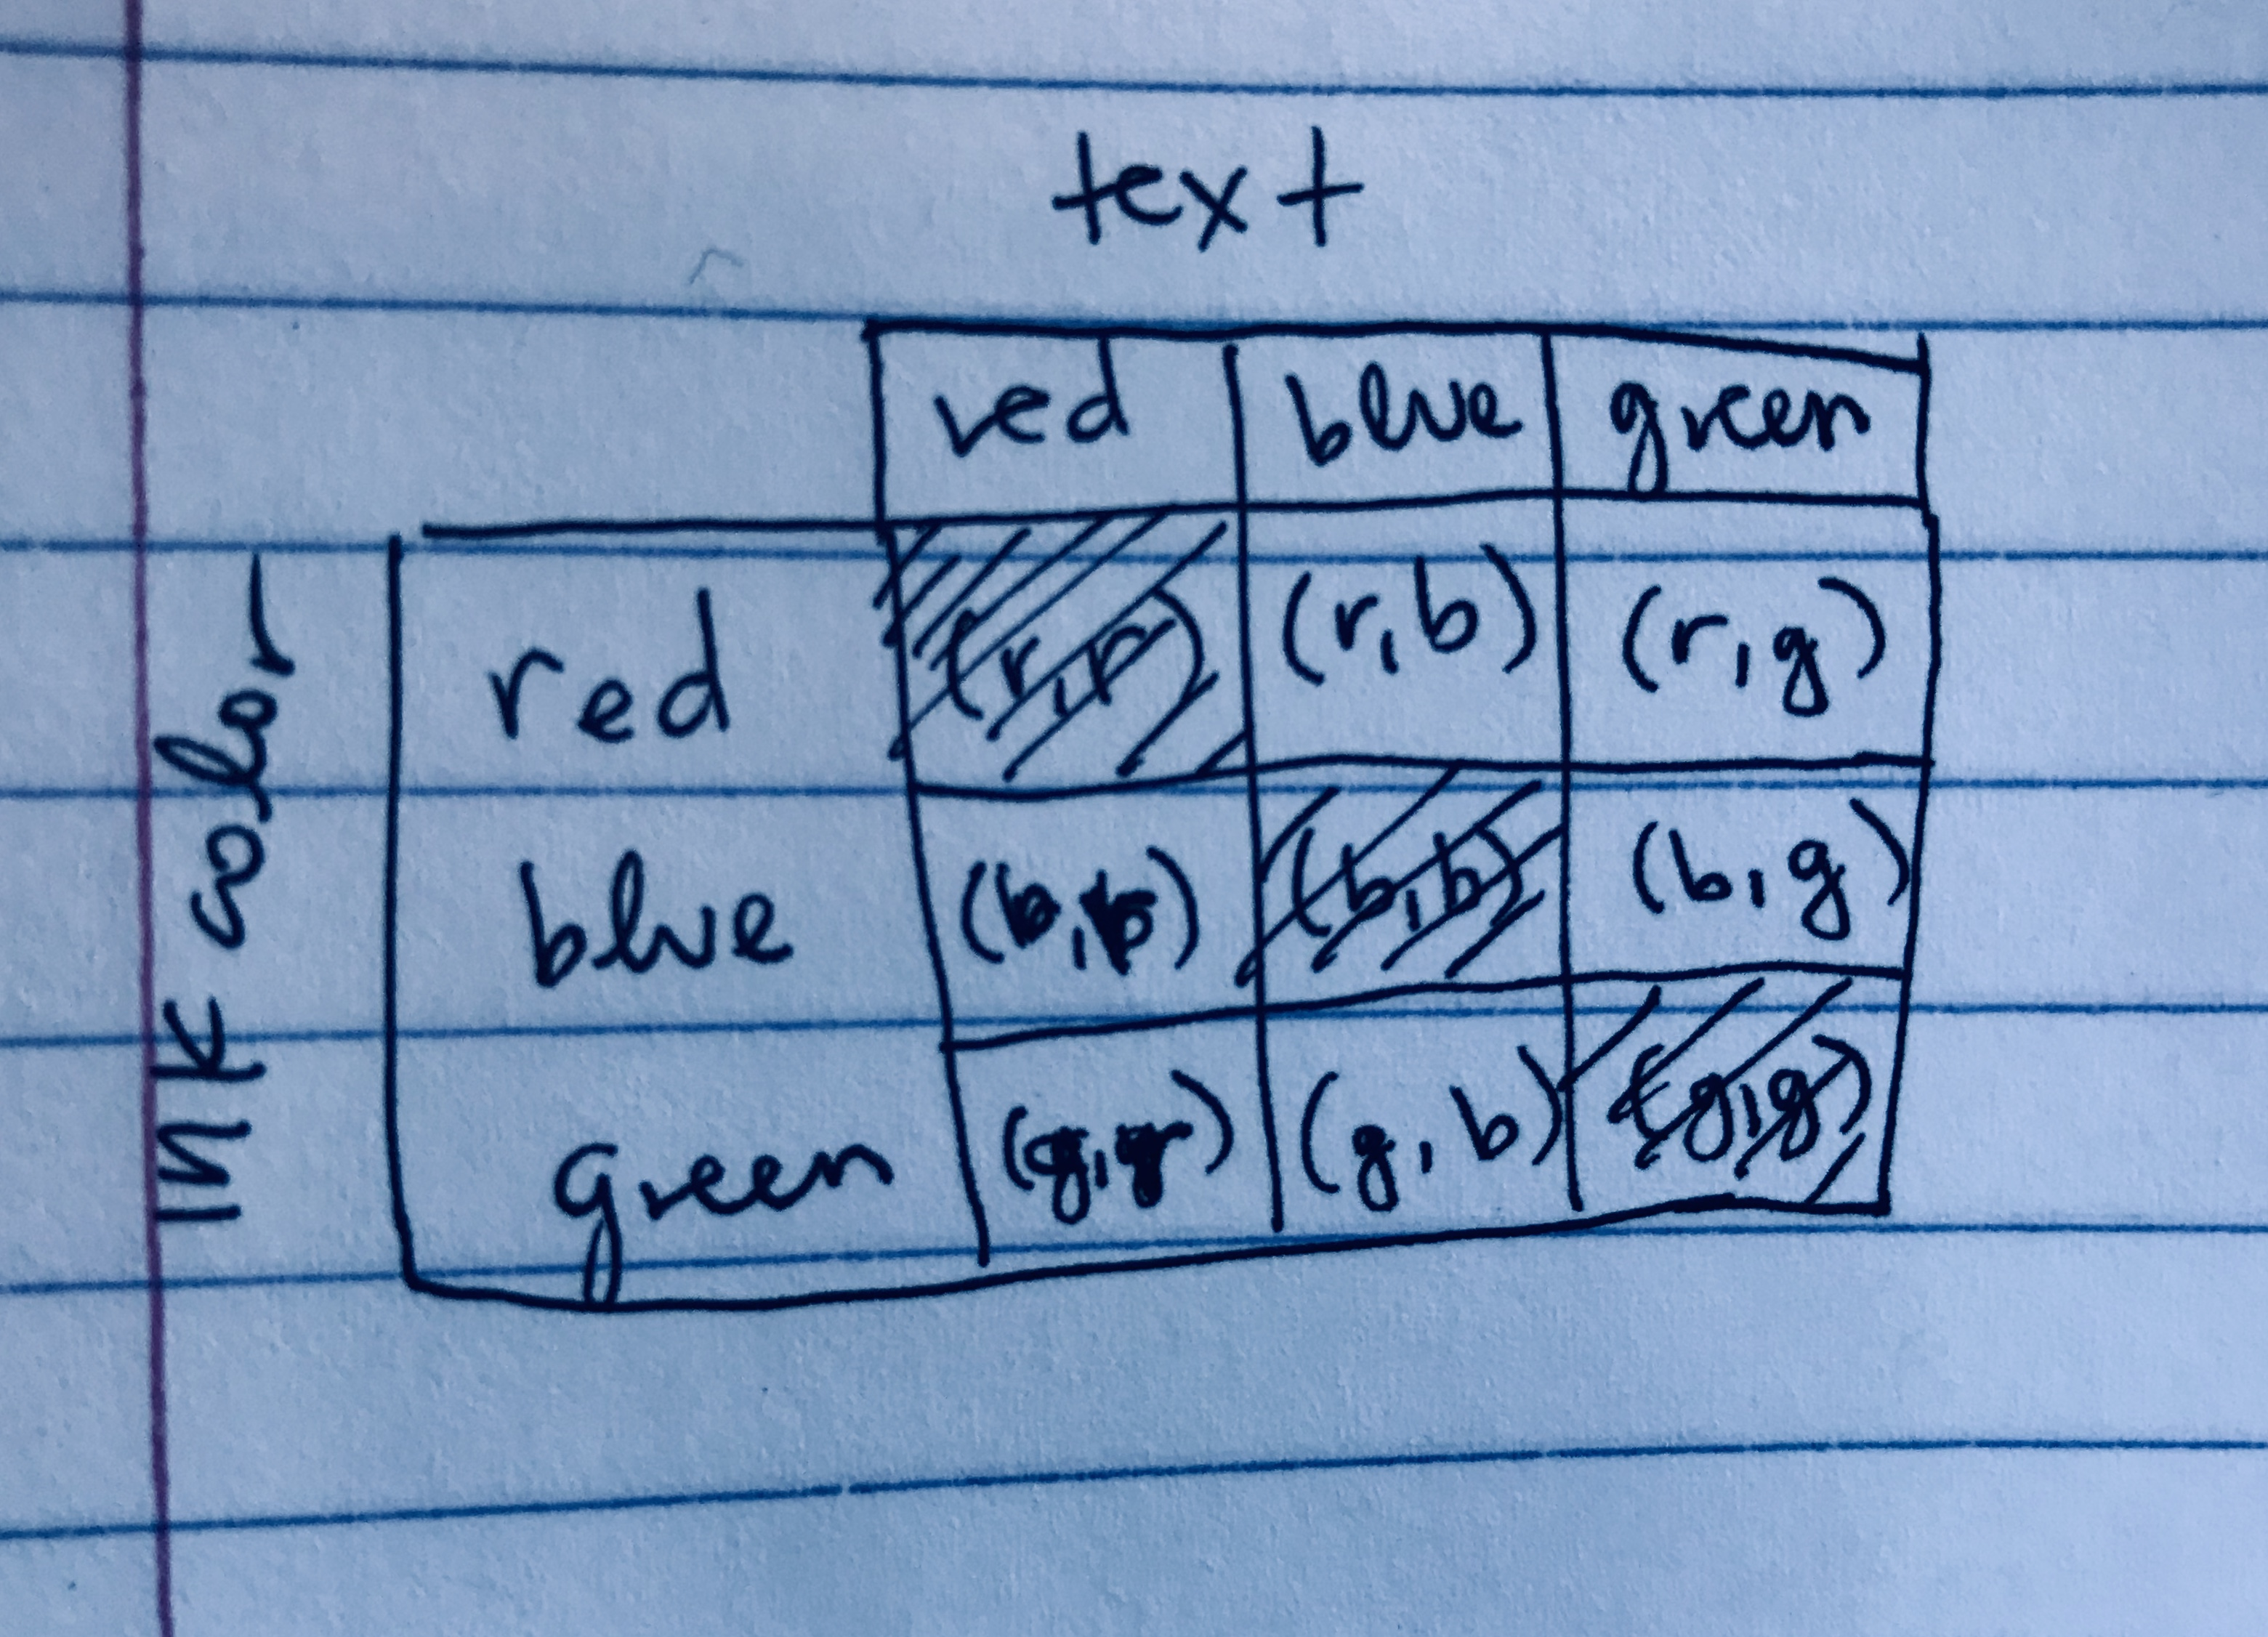
\includegraphics[origin=c,width=10cm]{fig_weighted_crossing}}
    \caption{Full crossing of a 3 color Stroop experiment. There are more congruent stimuli (along the diagonal) than incongruent stimuli.}%
    \label{fig:weighted_crossing}%
\end{figure}

\paragraph*{Sampling Continuous Factors}
Some experiments may contain levels which represent continuous values, such as sampling colors from the continuous color spectrum. We can currently represent these experiments by binning the continuous values into a number of discrete levels-- but can we do better? This is challenging because the translation to SAT is necessarily discrete. Perhaps this could be supported as a pre- and post- processing step, or perhaps Unigen could natively support this. The user could specify the continuous value, and SweetPea could perform binning, find a solution, and add random noise to the solution to simulate sampling from a continuous distribution.

\paragraph*{Automated Experimental Design}
In the spirit of declarative programming, it would be valuable to extend SweetPea to automatically derive the minimal set of counterbalancing conditions that satisfy the specified statistical analysis. Specifically, we may wish to provide an interface for the ANOVA (ANalysis Of VAriance) technique, which would allow researchers to state "contrast red with blue" instead of explicitly stating a design that does so. This higher-level interface will make it easier to specify experiments that accurately match the desired statistical analysis. Perhaps such an interface would also support iterative and interactive experiment specification. For instance, if multiple experiments match a desired statistical analysis, perhaps the user can use SweetPea to explore the options and tradeoffs of each of those possible experiments.

%\paragraph*{Syntactic Sugar}
%- don't have to write the name of the factor when the level name is unique


%%% ~~~~~~~~~~~~~~~~~~~~~~~~~~~~~~~~~~~~~~~~~~~~~~~~~~~~~~~~~~~~~~~~~~~~~~~~~~~
\section{Runtime Wishlist}

This section describes some runtime features which would facilitate a more interactive and usable environment.


\paragraph*{Verified Core}

SweetPea promises to make it easier to write correct experiments; this promise can only be true if SweetPea itself doesn't contain bugs. The boolean encoding parts of the code, especially the counting constraint encoding, is ripe for bugs because it produces a CNF formula, which is difficult for humans to read and verify. Currently, we protect against bugs through exhaustive testing. In the future it would be better to formally verify that these transformations are correct.

\paragraph*{Debugging unSAT experiments}

If a user writes down an experimental design which is overspecified, the SAT-sampler will state that the constraints are unsatisfiable. This is not as helpful as it could be-- why is it overspecified? Developing debugging support would create a more pleasant user experience. One possible approach is that some SAT-solvers can provide a \emph{minimally unsatisifiable core}, which specifies what set of variables lead to a contradicting assignment. It may be possible to use this minimally unsatisfiable core to translate back to which constraints over which the levels are reported to be contradictory.

\paragraph*{Iterative Experimental Design and Partial Satisfiability}

Extending the idea of adding support for debugging unsatisfiable experiments, it would be great to have SweetPea be a tool for exploring the edge of satisfiability. For instance, perhaps a researcher could attempt to specify an ambitious experimental design which tests multiple things at once: perhaps in the future SweetPea could allow them to iteratively explore which subsets of their overconstrained design are satisfiable. One technique for facilitating this is some SAT solvers allow you to push / pop individual clauses; perhaps this fine-grain precision can be used to find the most constraints which can be simultaneously satisfied.

% \paragraph*{Optimizations}
%
% Finally, there are some optimizations in that could be applied to the encodings discussed in Chapters 3, 4 and 5. A few examples are:
%
% Unigen supports "xor" constraints, in addition to the usual CNF formula. This is useful because adders are based on an "xor" operation internally. The current implementation desugars these xors into CNF, but perhaps explicitly specifying these xors might make the search simpler for the sampler, resulting in faster runtimes.
%
% The truth tables currently used to represent derivation functions can be compressed / optimized using the Quine-McCluskey algorithm. Further
%
% - choice of SAT encodings and variable v. clauses

\chapter{Conclusion}

This thesis presented SweetPea, a system for concisely describing experimental designs and rigerously generating experimental sequences that satisfy the design. SweetPea's high-level language allows scientists to declaratively describe the experiment they want to conduct rather than forcing them to mechanically describe how to construct their experimental sequences. This allows scientists to write concise, correct programs which describe their experiments, and produce unbiased experimental sequences; these programs can then be published and shared to document the experiment and facilitate replicability.


When a psychologist runs an experiment, it is important that the randomized experimental sequences that they show to the subjects represent a truely random sample of experimental sequences which express the experiment they are trying to run. Unfortunantly, it is difficult to construct these experimental sequences while guaranteeing that the construction isn't favoring certain sequences over others; this is an NP-hard problem for a large problem size. Currently psychologists

- Problem we tried to solve

- Why it's important

- What we did

- What are the consequences + forward looking

It is difficult to construct experimental sequences from randomized experimental designs while  This property, however, is also important



Creating randomized experimental designs while guaranteeing that the resulting experimental sequen



When psychologists test a hypothesis, they create an experimental design which expresses that experiment and then


% \numberofappendices = 1   % Set 0 for none, else number of appendices.
\numberofappendices = 0
%%% \appendix       % Chapters, sections are now appendix style A, A.1, A.2, B, C, D, ...

%%% %%% -*-LaTeX-*-

\chapter{The First}

This is an appendix.  Notice that the \LaTeX{} markup for an appendix
is, surprisingly, \verb=\chapter=.  The \verb=\appendix= command does
not produce a heading; instead, it just changes the numbering style
from numeric to alphabetic, and it changes the heading prefix from
\textbf{CHAPTER} to \textbf{APPENDIX}.

\blah \blah \blah

%%% %%% -*-LaTeX-*-

\chapter{The Second}

This is an appendix.

\blah \blah \blah

%%% %%% -*-LaTeX-*-

\chapter{The Third}

This is an appendix.

There are several books
\cite{%
    Singh:1997:FEE,%
    Salomon:1995:AT,%
    Robbins:2005:CSS,%
    Randell:1982:ODC,%
    Olver:2010:NHM,%
    Mittelbach:2004:LC,%
    Lamport:1985:LDP,%
    Knuth:1999:DT,%
    Knuth:1986:TB,%
    Knuth:1986:MB,%
    Farmelo:2009:SMH%
}
listed in our bibliography.

We also reference several journal articles
\cite{%
    Wiles:1995:MEC,%
    Taylor:1995:RTP,%
    Lahiri:2002:ADA,%
    Kim:1999:AFC,%
    Johnson:1978:LDT,%
    Huskey:1980:LLC,%
    Heilbron:1969:GBA,%
    Hall:1994:PNE,%
    Goldstine:1946:ENI,%
    Einstein:1911:BMAb,%
    Einstein:1911:BMAa,%
    Einstein:1906:NBM,%
    Cody:1981:APF,%
    Beebe:1989:PCP,%
    Babbage:1910:BBA%
}
and three famous doctoral theses of later winners
\cite{%
    Einstein:1905:NBM,%
    Dirac:1926:QM,%
    Bohr:1911:SME%
}
of the Nobel Prize in Physics (1922, 1933, and
1921):

Notice that, even though those citations appeared
in \LaTeX{} \verb=\cite{...}= commands with their
\BibTeX{} citation labels in reverse alphabetical
order, thanks to the \verb=citesort= package,
their reference-list numbers have been sorted in
numerically ascending order, and then
range-reduced.

Mention should also be made of a famous Dutch
computer scientist's first publication
\cite{Dijkstra:1953:FBV}.

Font metrics are an important, albeit low-level,
aspect of typesetting. See the \emph{Adobe
Systems} manual about that company's procedures
\cite{Adobe:1990:AFM}.

The bibliography at the end of this thesis contains several examples
of documents with non-English titles, and their \BibTeX{} entries
provide title translations following the practice recommended by the
American Mathematical Society and SIAM\@.  Here is a sample entry that
shows how to do so:
%
\begin{verbatim}
@PhdThesis{Einstein:1905:NBM,
  author =       "Albert Einstein",
  title =        "{Eine Neue Bestimmung der Molek{\"u}ldimensionen}.
                 ({German}) [{A} new determination of molecular
                 dimensions]",
  type =         "Inaugural dissertation",
  school =       "Bern Wyss.",
  address =      "Bern, Switzerland",
  year =         "1905",
  bibdate =      "Fri Dec 17 10:46:57 2004",
  bibsource =    "http://www.math.utah.edu/pub/tex/bib/einstein.bib",
  note =         "Published in \cite{Einstein:1906:NBM}.",
  acknowledgement = ack-nhfb,
  language =     "German",
  advisor =      "Alfred Kleiner (24 April 1849--3 July 1916)",
  URL =          "http://en.wikipedia.org/wiki/Alfred_Kleiner",
  remark =       "Received August 19, 1905 and published February 8,
                 1906.",
  Schilpp-number = "6",
}
\end{verbatim}

The \texttt{note} field in that entry refers to another bibliography
entry that need not have been directly cited in the document text.
Such cross-references are common in \BibTeX{} files, especially for
journal articles where there may be later comments and corrigenda that
should be mentioned.  Embedded \verb=\cite{}= commands ensure that
those possibly-important other entries are always included in the
reference list when the entry is cited.  The last bibliography entry
\cite{Wiles:1995:MEC} in this thesis has a long \texttt{note} field
that tells more about what some may view as the most important paper
in mathematics in the last century.

When entries cite other entries that cite other entries that cite
other entries that \ldots{}, multiple passes of \LaTeX{} and \BibTeX{}
are needed to ensure consistency.  That is another reason why document
compilation should be guided by a \texttt{Makefile} or a batch script,
rather than expecting the user to remember just how many passes are
needed.

\BibTeX{} entries are \emph{extensible}, in that arbitrary key\slash
value pairs may be present that are not necessarily recognized by any
bibliography style files.  The \texttt{advisor},
\texttt{acknowledgement}, \texttt{bibdate}, \texttt{bibsource},
\texttt{language}, \texttt{remark}, and \texttt{Schilpp-number} fields
are examples, and may be used by other software that processes
\BibTeX{} entries, or by humans who read the entries.  \texttt{DOI}
and \texttt{URL} fields are currently recognized by only a few styles,
but that situation will likely change as publishers demand that such
important information be included in reference lists.

In \BibTeX{} \texttt{title} fields, braces protect words, such as
proper nouns and acronyms, that cannot be downcased if the selected
bibliography style would otherwise do so.  In German, all nouns are
capitalized, and the simple way to ensure their protection is to brace
the entire German text in the title, as we did in the entry above.

The world's first significant computer program may
have been that written in 1842 by Lady Augusta Ada
Lovelace (1815--1852) for the computation of Bernoulli
numbers \cite{Huskey:1980:LLC,Kim:1999:AFC}.  She
was the assistant to Charles Babbage
(1791--1871), and they are the world's first
computer programmers. The programming language
\emph{Ada} is named after her, and is defined in
the ANSI/MIL-STD-1815A Standard; its number
commemorates the year of her birth.

We do not discuss mathematical \emph{transforms}
in this dissertation, but you can find that phrase
in the index (except that this sample thesis doesn't have one!)

\blah

\blah
\blah

\blah


%%% The choice of bibliography style is a major decision, jointly made
%%% by you, your thesis advisor and the thesis editor. Common choices are
%%% one of the four standard BibTeX styles (abbrv, alpha, plain, and unsrt),
%%% or enhanced styles like acm, amsplain, siam, and hundreds of others
%%% available in TeX Live, and other Unix and Windows TeX distributions.
%%%
%%% Do NOT handcode your reference list, because you are unlikely to
%%% achieve consistency or conformance to the University of Utah Thesis Office
%%% requirements: let BibTeX do that tedious job for you!
%%%
%%% Remember that reference-list metadata in BibTeX files remains
%%% constant across journals and publishers, and is are often reused
%%% in other documents and shared with others, whereas formatted
%%% reference-list styles change: with BibTeX, you only need to record
%%% the metadata once.
%%%
%%% If you prefer named, rather than numeric or tagged citations, you
%%% may use styles such as authordate{1,2,3,4}, chicago, harvard, or
%%% natbib.  Be aware, however, that most of those require an
%%% additional \usepackage{} command to supply \LaTeX{} with
%%% definitions of commands that the style needs, and that there are
%%% usually several flavors of LaTeX citation commands beyond the
%%% standard \cite{} command that you need to understand before you
%%% can use them properly in your prose.

%%% This tells BibTeX to read siam.bst from the first directory where
%%% it is found in the BSTINPUTS search path:

\bibliographystyle{siam}

%%% This can also specify a comma-separated list (without embedded
%%% spaces) of *.bib files found by BibTeX in its BIBINPUTS search
%%% path.  The argument \jobname means the base name of the top-level
%%% LaTeX file, avoiding an unnecessary filename dependence here.
%%%
%%% BibTeX writes only one .bbl file, no matter how many *.bib files
%%% are listed here, using the name \jobname.bbl.
%%%
%%% LaTeX reads BibTeX's formatted reference list from the file
%%% \jobname.bbl.

\bibliography{\jobname}

\end {document}
